\chapter{基于偏序协同对抗机制的涨跌分类研究}

\section{引言}

% ===== 第一段：研究背景与现实意义 =====
从高噪声、强非平稳的金融时间序列中提取有效预测信号，是量化交易的核心挑战。传统基于人工规则的策略难以应对海量数据，而数据驱动范式虽然在特征挖掘上展现出潜力，但金融数据的低信噪比特性依然限制了预测的稳定性。尤其是在股票、期货及多资产市场中，对未来价格方向（上涨或下跌）的分类预测不仅直接影响交易策略的构建，也在资产配置、风险管理以及执行优化等多个环节中发挥基础性作用。

早期金融预测研究主要基于统计学习方法，例如自回归模型（AR）、自回归滑动平均模型（ARMA）以及广义自回归条件异方差模型（GARCH）等。这类模型依赖严格的分布假设，能够刻画一定程度的线性结构与波动聚集特征，但在面对高维特征空间与复杂非线性关系时往往表现受限。Fama提出的有效市场假说（Efficient Market Hypothesis, EMH）进一步认为，市场价格已充分反映所有可获得信息，从而使得系统性超额收益难以持续获取\cite{fama1970efficient}。然而，大量后续研究表明，市场并非完全有效，动量效应、反转效应以及多因子溢价等现象均为可预测性提供了实证支持\cite{jegadeesh1993returns,carhart1997persistence}。

进入机器学习时代，研究者开始尝试使用支持向量机（SVM）、随机森林（Random Forest）和梯度提升树（GBDT）等方法进行方向预测。这些方法能够在一定程度上捕捉非线性关系，并通过特征工程提升模型表现。例如，Gu等人基于大规模横截面股票数据系统性比较了多种机器学习模型，发现树模型在收益预测任务中显著优于传统线性方法 \cite{gu2020empirical}。然而，这类方法仍高度依赖人工构造特征，其表达能力受限于预先设定的特征空间。

深度学习的兴起为金融预测提供了新的技术路径。与传统方法相比，深度神经网络能够通过多层非线性变换自动学习特征表示，从而减少对人工特征工程的依赖。特别是在图像识别与自然语言处理领域取得突破后，研究者开始将其迁移至金融时间序列建模中。Nelson等人较早地验证了深度神经网络在股票趋势预测中的潜力，表明其能够优于部分经典机器学习方法 \cite{nelson2017stock}。

在具体架构方面，循环神经网络（Recurrent Neural Networks, RNN）及其变体长短期记忆网络（LSTM）被广泛用于捕捉时间依赖结构。由于LSTM通过门控机制缓解了梯度消失问题，使得模型能够学习长期依赖关系，其在价格方向预测任务中表现出稳定优势 \cite{hochreiter1997long}。Fischer和Krauss基于标普500成分股数据构建LSTM模型，证明其在风险调整后收益上优于随机森林等基线方法 \cite{fischer2018deep}。

与此同时，卷积神经网络（CNN）也被用于金融预测。研究发现，一维卷积能够有效提取局部模式，而将技术指标转化为"图像"输入二维CNN则可以捕捉更高阶结构。Sezer与Ozbayoglu提出的CNN模型在方向预测任务中展现出一定的特征提取优势 \cite{sezer2018algorithmic}。

近年来，Transformer架构的出现进一步推动了序列建模能力的跃迁。基于自注意力机制，Transformer能够在无需递归结构的情况下捕捉全局依赖关系，从而显著提升并行计算效率。Vaswani等人提出该架构后，其在多个领域迅速成为主流方法 \cite{vaswani2017attention}。在金融场景中，Transformer被证明在多步预测与高维特征融合方面具有明显优势 \cite{zhou2021informer}。

% ===== 第二段：现有方法面临的核心挑战 =====
将深度学习直接应用于涨跌分类时，核心痛点在于：金融时间序列具有显著的非平稳性。市场结构、监管政策以及投资者行为均可能随时间发生变化，使得模型在训练期获得的模式难以长期泛化。此外，标签构造的不确定性进一步加剧了学习难度：简单地以未来收益符号作为标签可能引入噪声，而设置阈值则可能导致样本不平衡问题。

更关键的风险在于过拟合与数据泄露。由于金融数据通常具有强时间依赖性，不恰当的交叉验证方法可能导致模型在回测中表现优异但无法迁移至真实交易环境。近年来，越来越多研究强调应采用滚动窗口或扩展窗口等方式进行评估，以更接近真实部署场景 \cite{bailey2015pbo}。

另一个重要问题在于，可预测性并不必然转化为可交易性。即使分类准确率较高，如果忽略交易成本、滑点和市场冲击，策略仍可能无法实现正收益。因此，预测模型需要与执行机制协同设计，这一趋势正在推动执行感知学习的发展。

% ===== 第三段：本章研究的必要性与方向 =====
涨跌分类不仅是单纯的预测问题，更是连接信号生成与交易决策的关键桥梁。现有深度学习模型在应对金融市场非平稳性、维持模型多样性以及动态适应市场变化方面仍存在明显局限。现有的单一深度学习模型虽然在某些方面取得了进展，但在应对金融市场的非平稳性、模型多样性不足、以及缺乏动态适应机制等问题上仍存在局限。传统的简单集成方法（如硬投票）往往面临容错率低和错误放大的问题，因此，需要探索基于竞争与对抗机制的多模型协同、动态自适应的新框架，以进一步提升涨跌分类的稳定性和可交易性。

% ===== 第四段：本章贡献与章节结构安排 =====
基于上述背景，本章系统梳理深度学习在金融方向预测中的研究进展，并重点关注模型结构演化、标签设计、评估框架以及现实交易约束对预测性能的影响。相较于现有静态集成方法，针对静态集成方法在非平稳市场中容错率低的问题，本章构建了基于偏序协同对抗机制的涨跌分类框架。该框架通过群组交叉对抗与赛马场竞争机制，打破了固定权重集成的局限，实现了多智能体的动态优胜劣汰；同时结合双向师生蒸馏与孪生对抗检测，修复了复杂市场环境下的模式崩溃，最终在非平稳的金融时间序列中提供了更稳健的分类边界。本章所采用的多群组交叉对抗框架（MGCA）是第二章 MASA 核心思想在分类任务中的具体实例化，旨在验证对称对抗逻辑在预测一致性上的泛化能力。

本章后续内容安排如下：第2节梳理深度学习与多智能体在金融分类中的应用瓶颈；第3节详细推导偏序协同对抗架构及其核心机制的数学基础；第4节通过多资产实证验证该架构的泛化能力与抗崩溃特性；第5节深入探讨该机制在极端行情下的有效性与边界；第6节进行总结。

\section{相关工作}

\subsection{金融分类问题中的深度学习}

金融市场方向预测通常被建模为监督分类问题，即利用价格、成交量、盘口或因子暴露等历史信息预测未来收益方向。与连续收益回归相比，方向分类更易与交易规则、仓位控制和风险管理衔接，但金融序列的弱信号、强噪声与分布漂移也使其分类边界持续变化。

从研究演进看，方向分类经历了从逻辑回归、SVM 和树模型，到 LSTM、CNN、DeepLOB 与 Transformer 等深度模型的转变\cite{fischer2018deep,chen2019attlstm,sezer2018algorithmic,zhang2019DeepLOB,vaswani2017attention,ding2020hmsg,yoo2021dtml}。深度模型显著增强了时序表示与结构特征提取能力，但在极端行情、样本漂移和跨资产耦合场景下，单一模型仍缺乏足够的动态适应性。基于此，本章引入非对称的单生成器—多判别器协同对抗架构，以生成器构造边界样本、以多判别器协同稳定分类边界。

\subsection{金融分类中的集成学习与多智能体协同}

在高噪声、强非平稳环境下，单一模型容易过拟合或陷入局部最优，因此集成学习常被用于提升金融预测鲁棒性\cite{bailey2015pbo,gu2020empirical,lopezdeprado2018advances}。但无论是 Bagging、Boosting，还是基于不同初始化的深度集成，本质上多属于静态加权组合；一旦市场结构突变，固定权重就可能放大错误并导致样本外失效\cite{white2000realitycheck,hansen2005spa}。多智能体协同为此提供了新的思路：模型可在训练中竞争与合作，针对不同市场状态分工学习，并借助动态反馈保持多样性。基于这一考虑，本章通过赛马场竞争机制建立判别器间的动态秩序，使系统具备持续选择与自适应更新能力。

\subsection{对抗训练与知识蒸馏}

对抗训练通过生成器与判别器博弈学习数据分布，在金融领域常用于缓解样本不足和类别不平衡问题。但传统单生成器—单判别器结构在复杂时序上容易出现模式崩溃与训练发散，因此多判别器架构开始被用于提供更丰富的梯度信号。与此同时，知识蒸馏通过软标签与中间特征对齐提升模型泛化和置信度校准能力\cite{guo2017calibration}。现有方法的不足在于：蒸馏多为单向传递，多判别器 GAN 又常偏重生成质量而非分类收益。为此，本章将双向师生蒸馏（S2T）与孪生对抗检测（Twin）纳入偏序协同架构，以实现知识共享、异常修复和分类能力强化。

\section{方法论}

\subsection{问题定义与任务形式化}
本章的核心任务是基于高频限价指令簿（Limit Order Book, LOB）等时序数据进行未来价格趋势的分类预测。令 $X_t = [x_{t-T+1}, \dots, x_t] \in \mathbb{R}^{T \times F}$ 表示截止时刻 $t$ 的历史时间步序列，其中 $T$ 为时间窗口长度（本章设定为120），$F$ 为特征维度。我们的目标是学习一个映射函数 $f: \mathbb{R}^{T \times F} \rightarrow \mathbb{R}^3$，预测未来一定时间窗口内的价格变动趋势 $y_t \in \{0, 1, 2\}$，分别代表“跌”、“平”和“涨”。

为了提升分类模型的鲁棒性，本章将上述分类任务嵌入到生成对抗网络（GAN）框架中。令 $G$ 为生成器，$D$ 为判别器组。生成器的目标是学习真实市场数据分布 $P_{data}$，生成逼真的虚拟时序样本 $\hat{X} = G(z)$，其中 $z$ 为潜在噪声。判别器 $D$ 的任务被扩展为双重目标：首要任务是区分输入序列来自真实分布 \$P_{data}\$ 还是生成分布 \$P_G\$；更重要的是，针对真实样本 \$X_t\$，判别器必须最小化分类损失 $\mathcal{L}_{cls}(D(X_t), y_t)$。通过这种非对称的多组多成员博弈机制，生成器不断提供具有挑战性的边界样本，从而迫使判别器在对抗中学习到更具泛化能力的特征表示。

\subsection{偏序协同对抗架构}
针对金融时间序列预测中的收敛困难与模式崩溃问题，本章构建了基于偏序协同对抗架构的 MGCA 涨跌分类框架。该框架采用“单生成器 + 多判别器组”的非对称博弈结构：生成器学习市场微观结构并生成边界样本，多个异构判别器组负责真假判别与趋势分类。其训练核心为群组交叉对抗（GCA），并在此基础上依次叠加赛马场竞争（RT）、双向师生蒸馏（S2T）和孪生对抗检测（Twin），以实现优胜劣汰、知识迁移与异常修复。引入生成器的目的并非单纯生成序列，而是为分类器持续提供具有挑战性的边界样本，从而缓解有限样本下的过拟合。

\subsection{模型架构设计细节}
偏序协同对抗架构的设计兼顾了金融时序数据的复杂性与对抗博弈需求，整体采用非对称的多组多成员结构，以同时实现高质量序列生成与稳健趋势判别。

\subsubsection{生成器架构与多样性设计}
生成器负责捕捉市场微观结构并生成未来 OHLCV 序列。本文采用基于 Transformer 的 Seq2Seq 生成器，输入长度为120的历史窗口，通过4头自注意力、2层编码器和维度为512的前馈网络提取时序特征，再以自回归方式生成未来序列，Dropout 设为0.1。该设计能够同时刻画长程依赖与局部动态，为后续对抗训练提供高质量样本。

\subsubsection{判别器架构与双头输出机制}
判别器在MGCA框架中扮演着双重角色：既是区分真实与生成数据的“裁判”，也是预测未来趋势的“分析师”。为此，我们设计了支持CNN（卷积神经网络）和Transformer两种架构的时序分类网络。CNN判别器采用了多尺度1D卷积层，配合自适应平均池化层来提取局部特征；Transformer判别器则利用自注意力机制捕捉全局依赖。关键的创新在于判别器的双头输出机制（Dual-Head Output Mechanism）。

\begin{figure}[htbp]
\centering
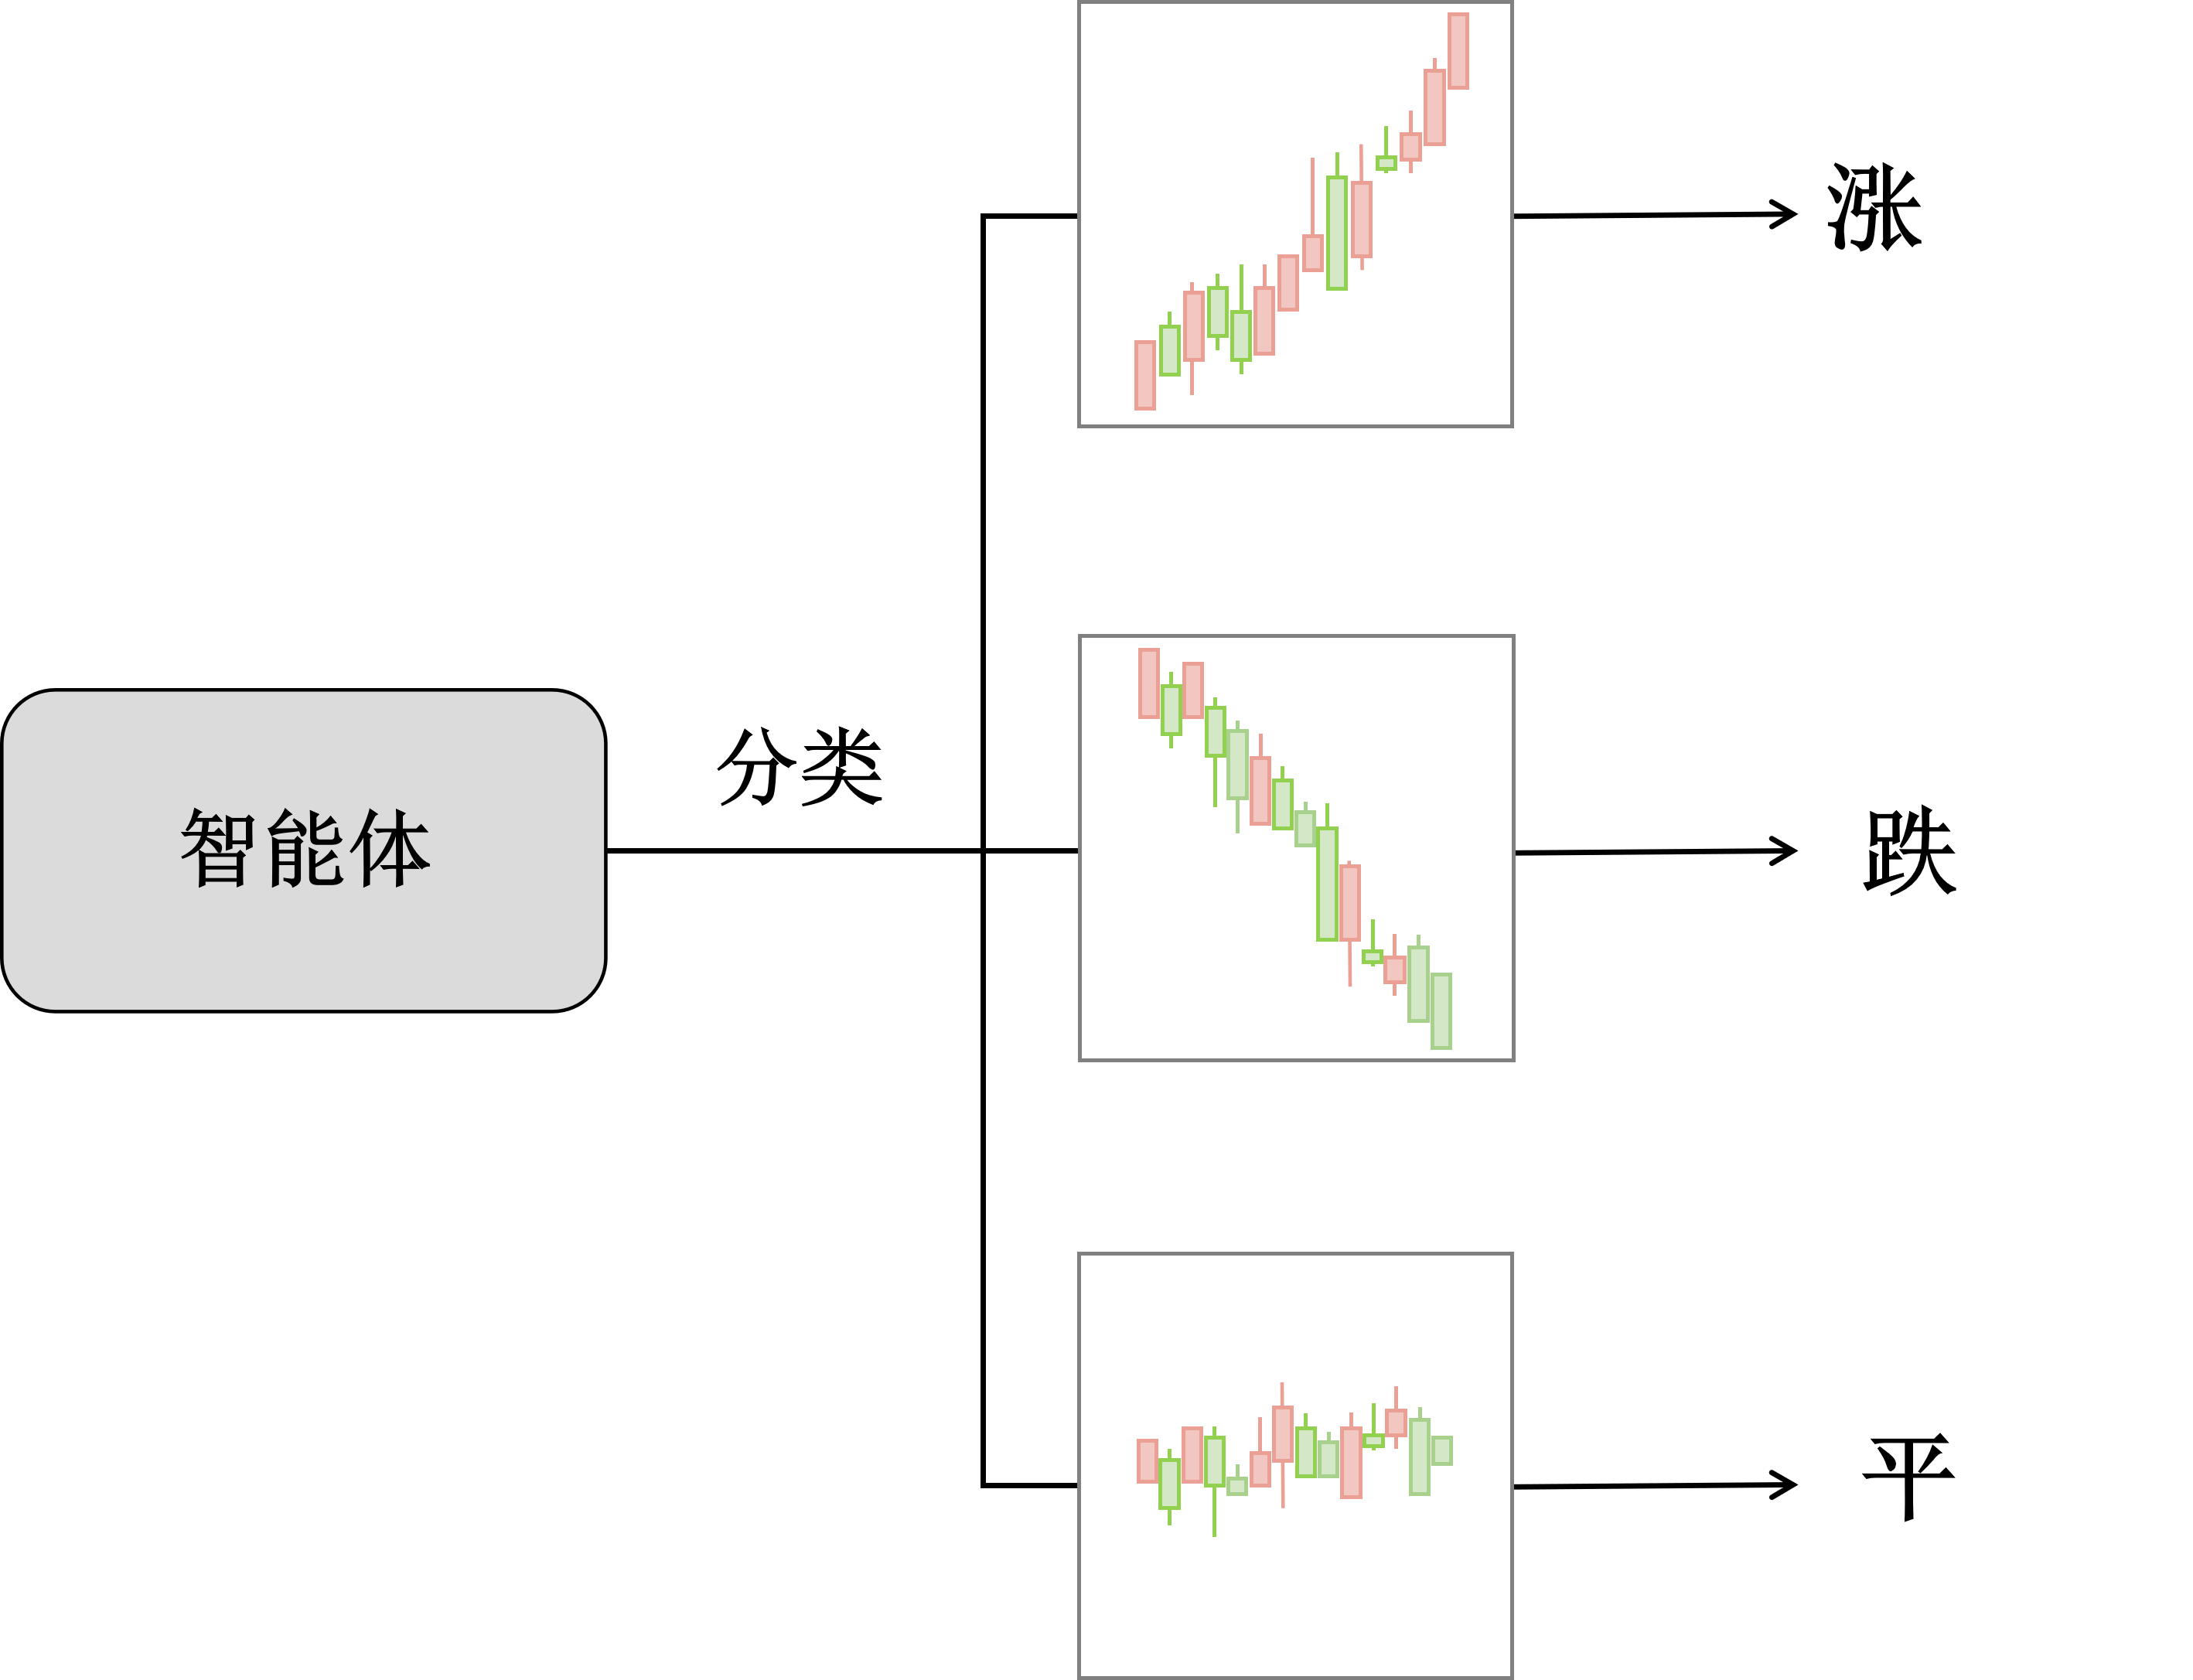
\includegraphics[width=0.5\textwidth]{figures/chap7/偏序/分类任务.png}
\caption{分类任务图}
\label{fig:twinclasstaskfig}
\end{figure}

如图\ref{fig:twinclasstaskfig}所示，不同于传统GAN判别器仅输出单一的真假标量，我们的判别器输出层包含两个关键分支：分类头（Classification Head）输出一个3维的Logits向量，对应未来价格的“涨、跌、平”三种趋势的概率分布，这使得判别器被迫理解市场的内在逻辑；特征头（Feature Head）直接输出倒数第二层的高维特征向量，为GCA和S2T阶段的特征级蒸馏提供了必要的载体，使得落后模型能够直接学习最优模型的内部表征。

\subsubsection{非对称多组多成员博弈配置}
架构的关键在于“1个生成器组 × 1个成员、2个判别器组 × 每组3个成员”的非对称配置。预训练后的单个 Transformer 生成器持续提供虚拟样本；两个判别器组中的6个异构判别器交替采用 CNN 与 Transformer 结构。该设计既引入组间竞争，又保留组内蒸馏与协作，使系统在生成—判别主线之外形成判别器之间的持续进化关系，并在部分成员失效时保持较强容错能力。

\subsubsection{复合损失体系}
在损失函数设计上，本文采用兼顾生成质量、分类精度与知识迁移的复合损失体系。

\textbf{（1）生成器金融感知重构损失。}生成器的核心损失函数为金融感知重构损失（Financial Aware Loss），该损失对OHLC价格维度与成交量维度采用不同的损失函数，以适应金融数据的异质性特征。价格维度采用Huber损失，其在误差较小时等价于MSE以保证平滑梯度，在误差较大时退化为线性损失以抑制价格跳变带来的梯度爆炸；成交量维度采用LogCosh损失，其对零值和异常值具有天然的鲁棒性。两者通过权重系数加权求和：

\begin{equation}
\mathcal{L}_{G}^{\text{recon}} = w_p \cdot \text{Huber}_{\delta=1.0}(\hat{P}_{\text{OHLC}}, P_{\text{OHLC}}) + w_v \cdot \text{LogCosh}(\hat{V}, V)
\label{eq:financial_aware_loss}
\end{equation}
其中$w_p=1.0$，$w_v=0.8$。Huber损失与LogCosh损失分别定义为：
\begin{equation}
\text{Huber}_\delta(e) = \begin{cases} \frac{1}{2}e^2, & |e| \leq \delta \\ \delta\left(|e| - \frac{1}{2}\delta\right), & |e| > \delta \end{cases}
\end{equation}
\begin{equation}
\text{LogCosh}(\hat{V}, V) = \frac{1}{N}\sum_{i=1}^{N}\log\left(\cosh(\hat{V}_i - V_i)\right)
\end{equation}

该设计突出价格信息的重要性，同时兼顾成交量这一辅助变量。

\textbf{（2）判别器分类损失。}判别器的损失函数采用基于三分类标签（涨/跌/平）的交叉熵损失（Cross-Entropy Loss）：

\begin{equation}
\mathcal{L}_{D}^{\text{CE}} = -\frac{1}{N}\sum_{i=1}^{N}\sum_{c=1}^{3} y_{i,c} \log(\hat{y}_{i,c})
\label{eq:disc_ce_loss}
\end{equation}

其中$c \in \{\text{涨}, \text{跌}, \text{平}\}$。相较于传统GAN中的二分类真假判别，这种设计迫使判别器不仅要区分数据的来源，更要深入理解市场的价格趋势逻辑。

\textbf{（3）知识蒸馏损失。}在GCA组内对抗、组间对抗以及S2T双向蒸馏环节中，落后判别器通过最小化与最优判别器在特征层和输出层的均方误差实现知识迁移：

\begin{equation}
\mathcal{L}_{\text{Distill}} = \lambda \cdot \left[\text{MSE}(\mathbf{f}_i, \mathbf{f}^*) + \text{MSE}(\mathbf{z}_i, \mathbf{z}^*)\right]
\label{eq:distill_loss}
\end{equation}

其中$\mathbf{f}_i$和$\mathbf{f}^*$分别为当前判别器和最优判别器倒数第二层的特征表示，$\mathbf{z}_i$和$\mathbf{z}^*$为对应的输出层Logits，蒸馏权重系数$\lambda=0.1$。这一设计在保持判别器多样性的同时引导其向最优解收敛。

\textbf{（4）赛马场学生蒸馏损失。}在RT赛马场阶段，新初始化的学生判别器通过拟合所有现有判别器的集成输出实现快速知识吸收：

\begin{equation}
\mathcal{L}_{\text{Student}} = \mathcal{L}_D^{\text{CE}} + \lambda \cdot \text{MSE}\left(\mathbf{z}_{\text{student}},\; \frac{1}{K}\sum_{k=1}^{K}\mathbf{z}_k\right)
\label{eq:rt_student_loss}
\end{equation}

其中$K$为所有判别器的总数，$\mathbf{z}_k$为第$k$个判别器的输出，$\lambda=0.1$。

\textbf{（5）GAN对抗微调损失。}在Twin孪生对抗检测阶段的最终微调中，生成器与判别器的损失函数分别为：
\begin{equation}
\mathcal{L}_{G}^{\text{finetune}} = \mathcal{L}_{G}^{\text{recon}} + 0.1 \times \mathcal{L}_{D}^{\text{CE}}(D_{\text{best}}(G(\mathbf{x})), \mathbf{y})
\label{eq:gan_finetune_g}
\end{equation}
\begin{equation}
\mathcal{L}_{D}^{\text{finetune}} = \mathcal{L}_{D}^{\text{CE}}(D_{\text{best}}(\mathbf{x}), \mathbf{y})
\label{eq:gan_finetune_d}
\end{equation}

生成器损失同时约束重构质量与对抗能力，判别器损失则聚焦最终分类精度。

\subsection{偏序协同训练机制与模块化流程}
本节说明偏序协同架构的基本训练机制及三项增强模块（RT、S2T、Twin）。其中，GCA 为基础训练范式，后三者是在此之上按需启用的增强步骤。

\subsubsection{偏序协同架构基本训练：群组交叉对抗（GCA）}
群组交叉对抗（GCA）是偏序协同架构的基础训练机制，负责完成生成器预训练并建立判别器的组内、组间竞争秩序。首先，生成器在金融感知重构损失约束下学习 OHLCV 的基本形态；随后生成虚拟样本，并按 $fake\_ratio$ 与真实数据混合，构造判别器训练所需的半真实数据环境。接着，在组内训练中，各判别器并行学习分类任务，并依据验证集 CE 损失选出组内最优成员，其余成员通过特征和 Logits 蒸馏向其靠拢。最后，各组代表再进行组间比较，由全局最优判别器引导跨组蒸馏，从而实现从局部最优到全局更优的收敛。

\subsubsection{赛马场竞争机制（RT）}
在 GCA 建立的秩序基础上，赛马场竞争（RT）进一步引入外部竞争机制。系统重新构造混合数据集，先定位全局最优与最差判别器，再以最优模型结构初始化“新学生”。该学生不仅学习真实标签，还拟合所有判别器的平均输出，以吸收集体知识；训练完成后，用其替换全局最差成员，并输出更新后的判别器矩阵。

\subsubsection{双向师生蒸馏（S2T）}
双向师生蒸馏（S2T）旨在打破传统蒸馏的单向传递限制。该阶段先评估各判别器并确定初始最优者 $a_1$ 与最差者 $b_1$，随后在混合数据上继续训练所有成员；重新评分后，以新的全局最优者 $a_2$ 为中心执行常规蒸馏。进一步地，系统将 $b_1$ 位置成员视为“学生”，其余视为“教师”，根据 CE 差异和阈值 $\theta$ 决定是学生向教师学习，还是当学生显著超越教师时触发反向蒸馏。该机制使知识在群体中双向流动，从而增强差异化互补。

\subsubsection{孪生对抗检测（Twin）}
孪生对抗检测（Twin）是系统的最终稳定器。该阶段统计各判别器相对最优判别器的超阈值次数；当某成员的异常频次达到 $twins\_threshold$，且系统中仍存在其他正常判别器组时，即判定其已偏离正常轨迹。随后，系统用当前最优判别器及其优化器状态进行深拷贝替换，并安排生成器与最优判别器进行一轮 GAN 微调，以恢复整体鲁棒性。

\subsection{算法流程与伪代码描述}
为更清晰展示 MGCA 的训练逻辑，本节将上述机制写成形式化算法流程。整体训练遵循严格的偏序执行策略：先完成初始化与 GCA 基础训练，再按配置依次进入 RT、S2T 与 Twin 阶段，并在每一步更新全局最优状态作为下一阶段输入，以减少多目标优化中的震荡。

\subsubsection{总体训练流程}
总体流程包括初始化生成器组与判别器组、执行 GCA 基础训练，并在此后按配置选择性启用 RT、S2T 与 Twin 三个模块。模块化且有序的调用方式保证了训练过程的稳定性与可控性。

\begin{algorithm}[H]
\caption{MGCA框架总体训练流程}
\label{alg:mgca}
\begin{algorithmic}[0]
\Require 数据集 $\mathcal{D}$（训练集/验证集/测试集），生成器组 $\mathcal{G}$（1组，1个成员），判别器组 $\mathcal{D}_{\text{groups}}$（2组，每组3个成员）
\Ensure 训练好的生成器 $\mathcal{G}_{\text{trained}}$，最优判别器 $\mathcal{D}_{\text{best}}$
\Statex
\State \textbf{/* 初始化 */}
\State 使用随机权重初始化 $\mathcal{G}$ 和 $\mathcal{D}_{\text{groups}}$
\State 配置优化器：$\text{Opt}_{\mathcal{G}}$（学习率=$4\times10^{-5}$），$\text{Opt}_{\mathcal{D}}$（学习率=$2\times10^{-5}$）
\Statex
\State \textbf{/* 偏序协同架构基本训练：群组交叉对抗（GCA） */}
\State $\mathcal{G}_{\text{trained}}, \mathcal{D}_{\text{global-best}} \gets \text{Execute-GCA}(\mathcal{G}, \mathcal{D}_{\text{groups}}, \mathcal{D})$
\Statex
\State \textbf{/* 创新点一：赛马场竞争（RT） */}
\If{启用RT}
    \State $\mathcal{D}_{\text{global-best}} \gets \text{Execute-RT}(\mathcal{G}_{\text{trained}}, \mathcal{D}_{\text{groups}}, \mathcal{D}_{\text{global-best}})$
\EndIf
\Statex
\State \textbf{/* 创新点二：双向师生蒸馏（S2T） */}
\If{启用S2T}
    \State $\mathcal{D}_{\text{global-best}} \gets \text{Execute-S2T}(\mathcal{D}_{\text{groups}}, \mathcal{D}_{\text{global-best}})$
\EndIf
\Statex
\State \textbf{/* 创新点三：孪生对抗检测（Twin） */}
\If{启用Twin}
    \State $\mathcal{G}_{\text{trained}}, \mathcal{D}_{\text{best}} \gets \text{Execute-Twin}(\mathcal{G}_{\text{trained}}, \mathcal{D}_{\text{groups}}, \mathcal{D}_{\text{global-best}})$
\Else
    \State $\mathcal{D}_{\text{best}} \gets \mathcal{D}_{\text{global-best}}$
\EndIf
\Statex
\State \Return $\mathcal{G}_{\text{trained}}, \mathcal{D}_{\text{best}}$
\end{algorithmic}
\end{algorithm}

% \begin{algorithm}
% \caption{MGCA Framework Overall Training Process}
% \label{alg:mgca}
% \begin{algorithmic}[1]
% \Require 
%     Dataset $\mathcal{D}$ (Train/Val/Test), 
%     Generator Group $\mathcal{G}$ (1 group, 3 members), 
%     Discriminator Groups $\mathcal{D}_{\text{groups}}$ (2 groups, 3 members/group)
% \Ensure 
%     Best Generator $\mathcal{G}_{\text{best}}$, Best Discriminator $\mathcal{D}_{\text{best}}$
% \Statex
% \Comment{Initialization}
% \State Initialize $\mathcal{G}$ and $\mathcal{D}_{\text{groups}}$ with random weights
% \State Configure Optimizers: $\text{Opt}_\mathcal{G}$ (lr=$1\times10^{-3}$), $\text{Opt}_\mathcal{D}$ (lr=$1\times10^{-4}$)
% \Statex
% \Comment{Step 1: Group Cross-Adversarial (GCA)}
% \State $\mathcal{G}_{\text{best}}, \mathcal{D}_{\text{global\_best}} \gets \text{Execute\_GCA}(\mathcal{G}, \mathcal{D}_{\text{groups}}, \mathcal{D})$
% \Statex
% \Comment{Step 2: Racetrack Competition (RT)}
% \If {Enable\_RT}
%     \State $\mathcal{D}_{\text{global\_best}} \gets \text{Execute\_RT}(\mathcal{G}_{\text{best}}, \mathcal{D}_{\text{groups}}, \mathcal{D}_{\text{global\_best}})$
% \EndIf
% \Statex
% \Comment{Step 3: Student-to-Teacher Bidirectional Distillation (S2T)}
% \If {Enable\_S2T}
%     \State $\mathcal{D}_{\text{global\_best}} \gets \text{Execute\_S2T}(\mathcal{D}_{\text{groups}}, \mathcal{D}_{\text{global\_best}})$
% \EndIf
% \Statex
% \Comment{Step 4: Twin Adversarial Detection (Twin)}
% \If {Enable\_Twin}
%     \State $\mathcal{G}_{\text{best}}, \mathcal{D}_{\text{best}} \gets \text{Execute\_Twin}(\mathcal{G}_{\text{best}}, \mathcal{D}_{\text{groups}}, \mathcal{D}_{\text{global\_best}})$
% \Else
%     \State $\mathcal{D}_{\text{best}} \gets \mathcal{D}_{\text{global\_best}}$
% \EndIf
% \Statex
% \State \Return $\mathcal{G}_{\text{best}}, \mathcal{D}_{\text{best}}$
% \end{algorithmic}
% \end{algorithm}

\subsubsection{各阶段详细算法描述}
GCA 阶段的核心在于通过组内与组间两层蒸馏实现优胜劣汰。生成器先在金融感知损失约束下预训练，再生成虚拟数据构造混合样本；随后各判别器先向组内最优者对齐，再由各组代表向全局最优者对齐，从而推动系统由局部最优逐步收敛至更优解。

\begin{algorithm}[H]
\caption{偏序协同架构基本训练 - 群组交叉对抗（GCA）}
\label{alg:gca}
\begin{algorithmic}[0]
\State \textbf{阶段1：生成器预训练}
\For{epoch $\in$ Init\_Epochs}
    \State $\text{Loss}_G = \text{Financial\_Aware\_Loss}(G(x), \text{real\_x})$
    \State 使用 $\text{Loss}_G$ 更新生成器 $G$
\EndFor
\State 上述步骤训练完成后得到训练好的生成器$\mathcal{G}_{\text{trained}}$
\Statex
\State \textbf{阶段2：混合数据生成}
\State $\text{Data\_Mixed} = \text{Mix}(\text{Real\_Data},\; \mathcal{G}_{\text{trained}}(x),\; \text{ratio}=1-\text{fake\_ratio})$
\Statex
\State \textbf{阶段3：组内对抗}
\For{$D_{\text{groups}}$ 中的每个组}
    \State 在 $\text{Data\_Mixed}$ 上训练组内所有判别器
    \State 在验证集上评估，选出组内最优 $\text{Group\_Best}$（CE最小）
    \For{组内每个判别器}
        \If{该判别器 $\neq$ $\text{Group\_Best}$}
            \State $\text{Loss}_{\text{Distill}} = \text{MSE}(\text{Feat}, \text{Group\_Best.Feat}) + \text{MSE}(\text{Logits}, \text{Group\_Best.Logits})$
            \State 使用 $\text{Loss}_{\text{Distill}}$ 更新该判别器
        \EndIf
    \EndFor
\EndFor
\Statex
\State \textbf{阶段4：组间对抗}
\State 从所有 $\text{Group\_Best}$ 中选出全局最优 $\text{Global\_Best}$
\For{每个 $\text{Group\_Best}$}
    \If{$\text{Group\_Best} \neq \text{Global\_Best}$}
        \State $\text{Loss}_{\text{Distill}} = \text{MSE}(\text{Feat}, \text{Global\_Best.Feat}) + \text{MSE}(\text{Logits}, \text{Global\_Best.Logits})$
        \State 使用 $\text{Loss}_{\text{Distill}}$ 更新 $\text{Group\_Best}$
    \EndIf
\EndFor
\end{algorithmic}
\end{algorithm}

\begin{figure}[htbp]
    \centering
    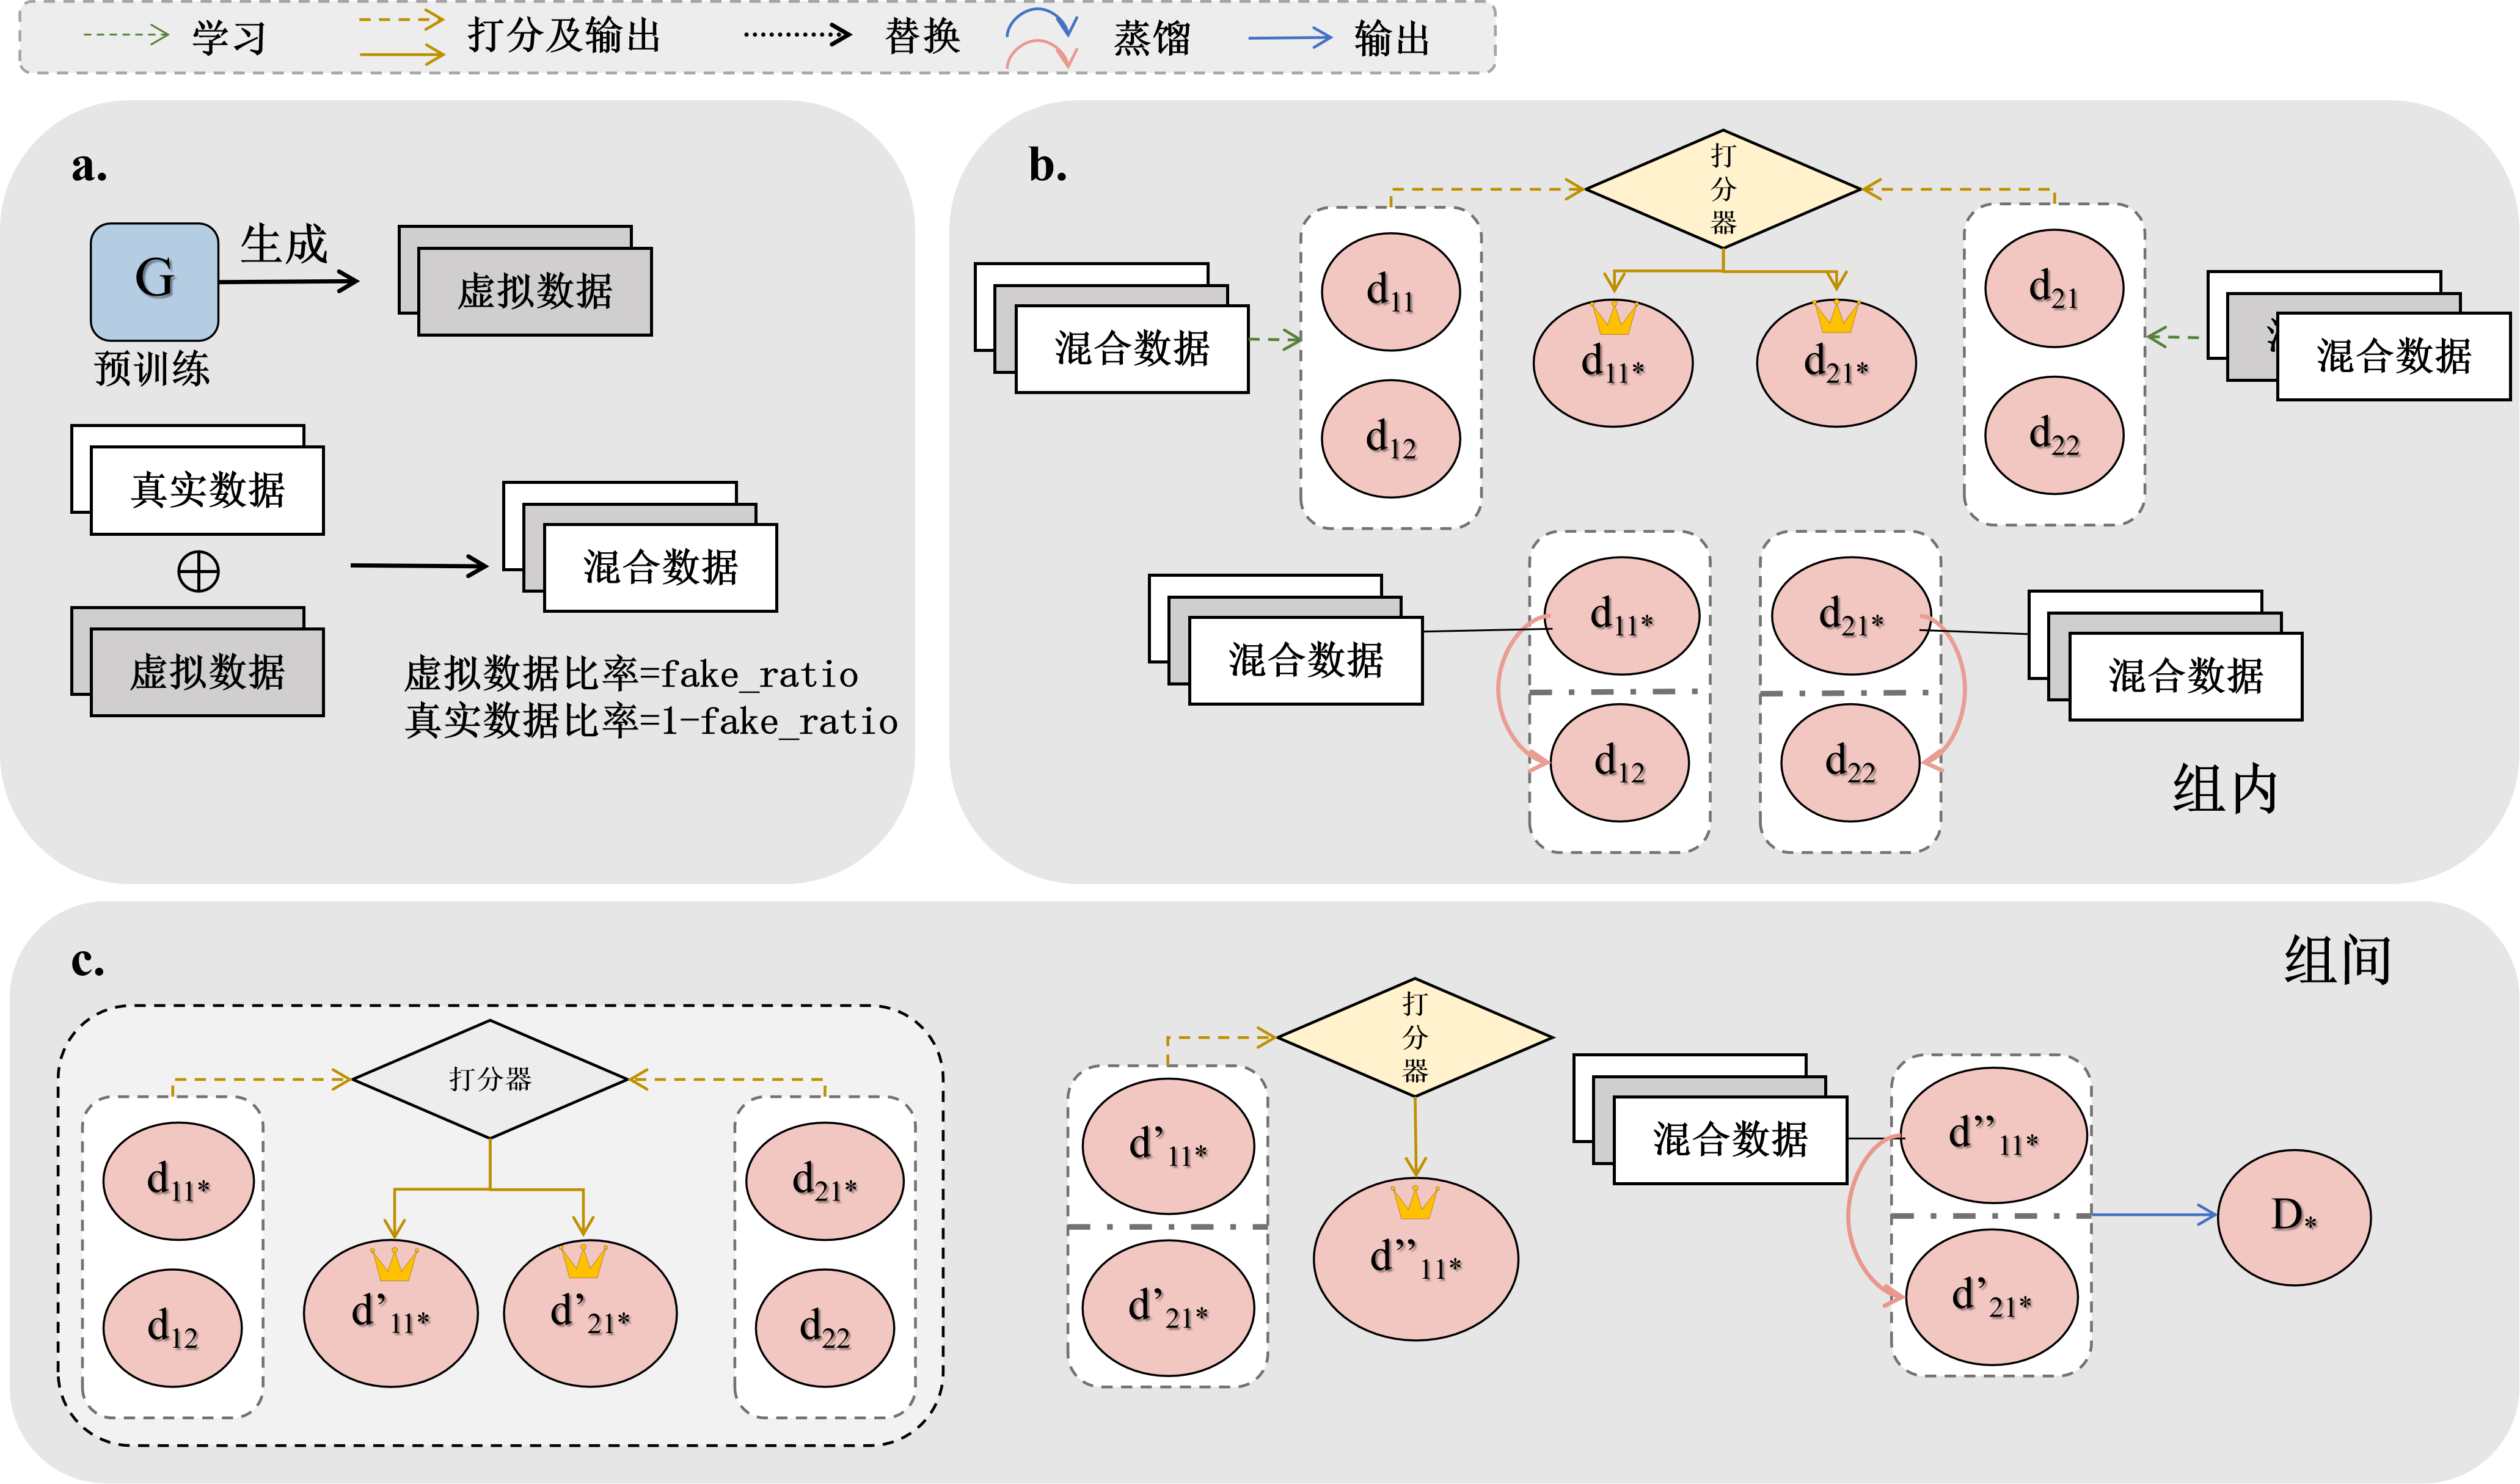
\includegraphics[width=0.8\textwidth]{figures/chap7/偏序/群组偏序.png}
    \caption{偏序协同对抗机制下的群组交叉对抗训练流程示意图}
    \label{fig:GCA-Partial-GCA}
\end{figure}

% \begin{algorithm}
% \caption{Step 1 - Group Cross-Adversarial (GCA)}
% \label{alg:gca}
% \begin{algorithmic}[1]
% \State \textbf{Stage 1: Generator Pre-training}
% \For{epoch $\in$ Init\_Epochs}
%     \State $\text{Loss}_G = \text{Financial\_Aware\_Loss}(G(x), \text{real\_x})$
%     \State Update $G$ with $\text{Loss}_G$
% \EndFor
% \State
% \State \textbf{Stage 2: Mixed Data Generation}
% \State $\text{Data\_Mixed} = \text{Mix}(\text{Real\_Data}, G(x), \text{ratio}=1-\text{fake\_ratio})$
% \State
% \State \textbf{Stage 3: Intra-Group Adversarial}
% \For{each Group in $D_{\text{groups}}$}
%     \State Train all discriminators on $\text{Data\_Mixed}$
%     \State Evaluate on $\text{Val\_Set}$, identify $\text{Group\_Best}$ (lowest CE)
%     \For{each discriminator in Group}
%         \If{discriminator $\neq$ $\text{Group\_Best}$}
%             \State $\text{Loss}_{\text{Distill}} = \text{MSE}(\text{Feat}, \text{Group\_Best.Feat}) + \text{MSE}(\text{Logits}, \text{Group\_Best.Logits})$
%             \State Update discriminator with $\text{Loss}_{\text{Distill}}$
%         \EndIf
%     \EndFor
% \EndFor
% \State
% \State \textbf{Stage 4: Inter-Group Adversarial}
% \State Identify $\text{Global\_Best}$ among all $\text{Group\_Bests}$
% \For{each $\text{Group\_Best}$}
%     \If{$\text{Group\_Best} \neq \text{Global\_Best}$}
%         \State $\text{Loss}_{\text{Distill}} = \text{MSE}(\text{Feat}, \text{Global\_Best.Feat}) + \text{MSE}(\text{Logits}, \text{Global\_Best.Logits})$
%         \State Update $\text{Group\_Best}$ with $\text{Loss}_{\text{Distill}}$
%     \EndIf
% \EndFor
% \end{algorithmic}
% \end{algorithm}
        
赛马场竞争机制（RT）是本章的第一个创新点。赛马场（RT）阶段引入了外部的“鲶鱼效应”。算法首先评估当前所有判别器，锁定最差者。随后，初始化一个全新的“学生”判别器，该学生在训练时不仅学习真实标签，还通过集成学习的方式拟合所有现有判别器的平均输出，从而快速掌握集体智慧。训练完成后，该学生直接替换掉系统中的最差判别器，并重置优化器，从而强制系统跳出可能存在的局部极值陷阱。

\begin{algorithm}[H]
\caption{赛马场竞争机制（RT）算法流程}
\label{alg:racetrack}
\begin{algorithmic}[0]
\State \textbf{阶段1\&2：评估与定位}
\State 评估所有判别器，找到全局最差 $\texttt{Global\_Worst}$ 和全局最优 $\texttt{Global\_Best}$
\Statex
\State \textbf{阶段3：训练新学生}
\State 初始化 $\texttt{Student\_D}$（深拷贝 $\texttt{Global\_Best}$）
\For{$\texttt{Mixed\_Data}$ 中的每个批次}
    \State $\texttt{Teacher\_Ensemble} \gets \text{Average}(\text{All\_Discriminators}(\text{batch}))$
    \State $\text{Loss\_Student} \gets \text{CE}(\texttt{Student\_D}(\text{batch}), \text{label}) + \lambda \cdot \text{MSE}(\texttt{Student\_D}(\text{batch}), \texttt{Teacher\_Ensemble})$
    \State 更新 $\texttt{Student\_D}$
\EndFor
\Statex
\State \textbf{阶段4\&5：替换}
\State 使用 $\texttt{Student\_D}$ 替换 $\texttt{Global\_Worst}$
\State 重置被替换位置的优化器
\State 重新评估并更新 $\texttt{Global\_Best}$
\end{algorithmic}
\end{algorithm}

\begin{figure}[htbp]
    \centering
    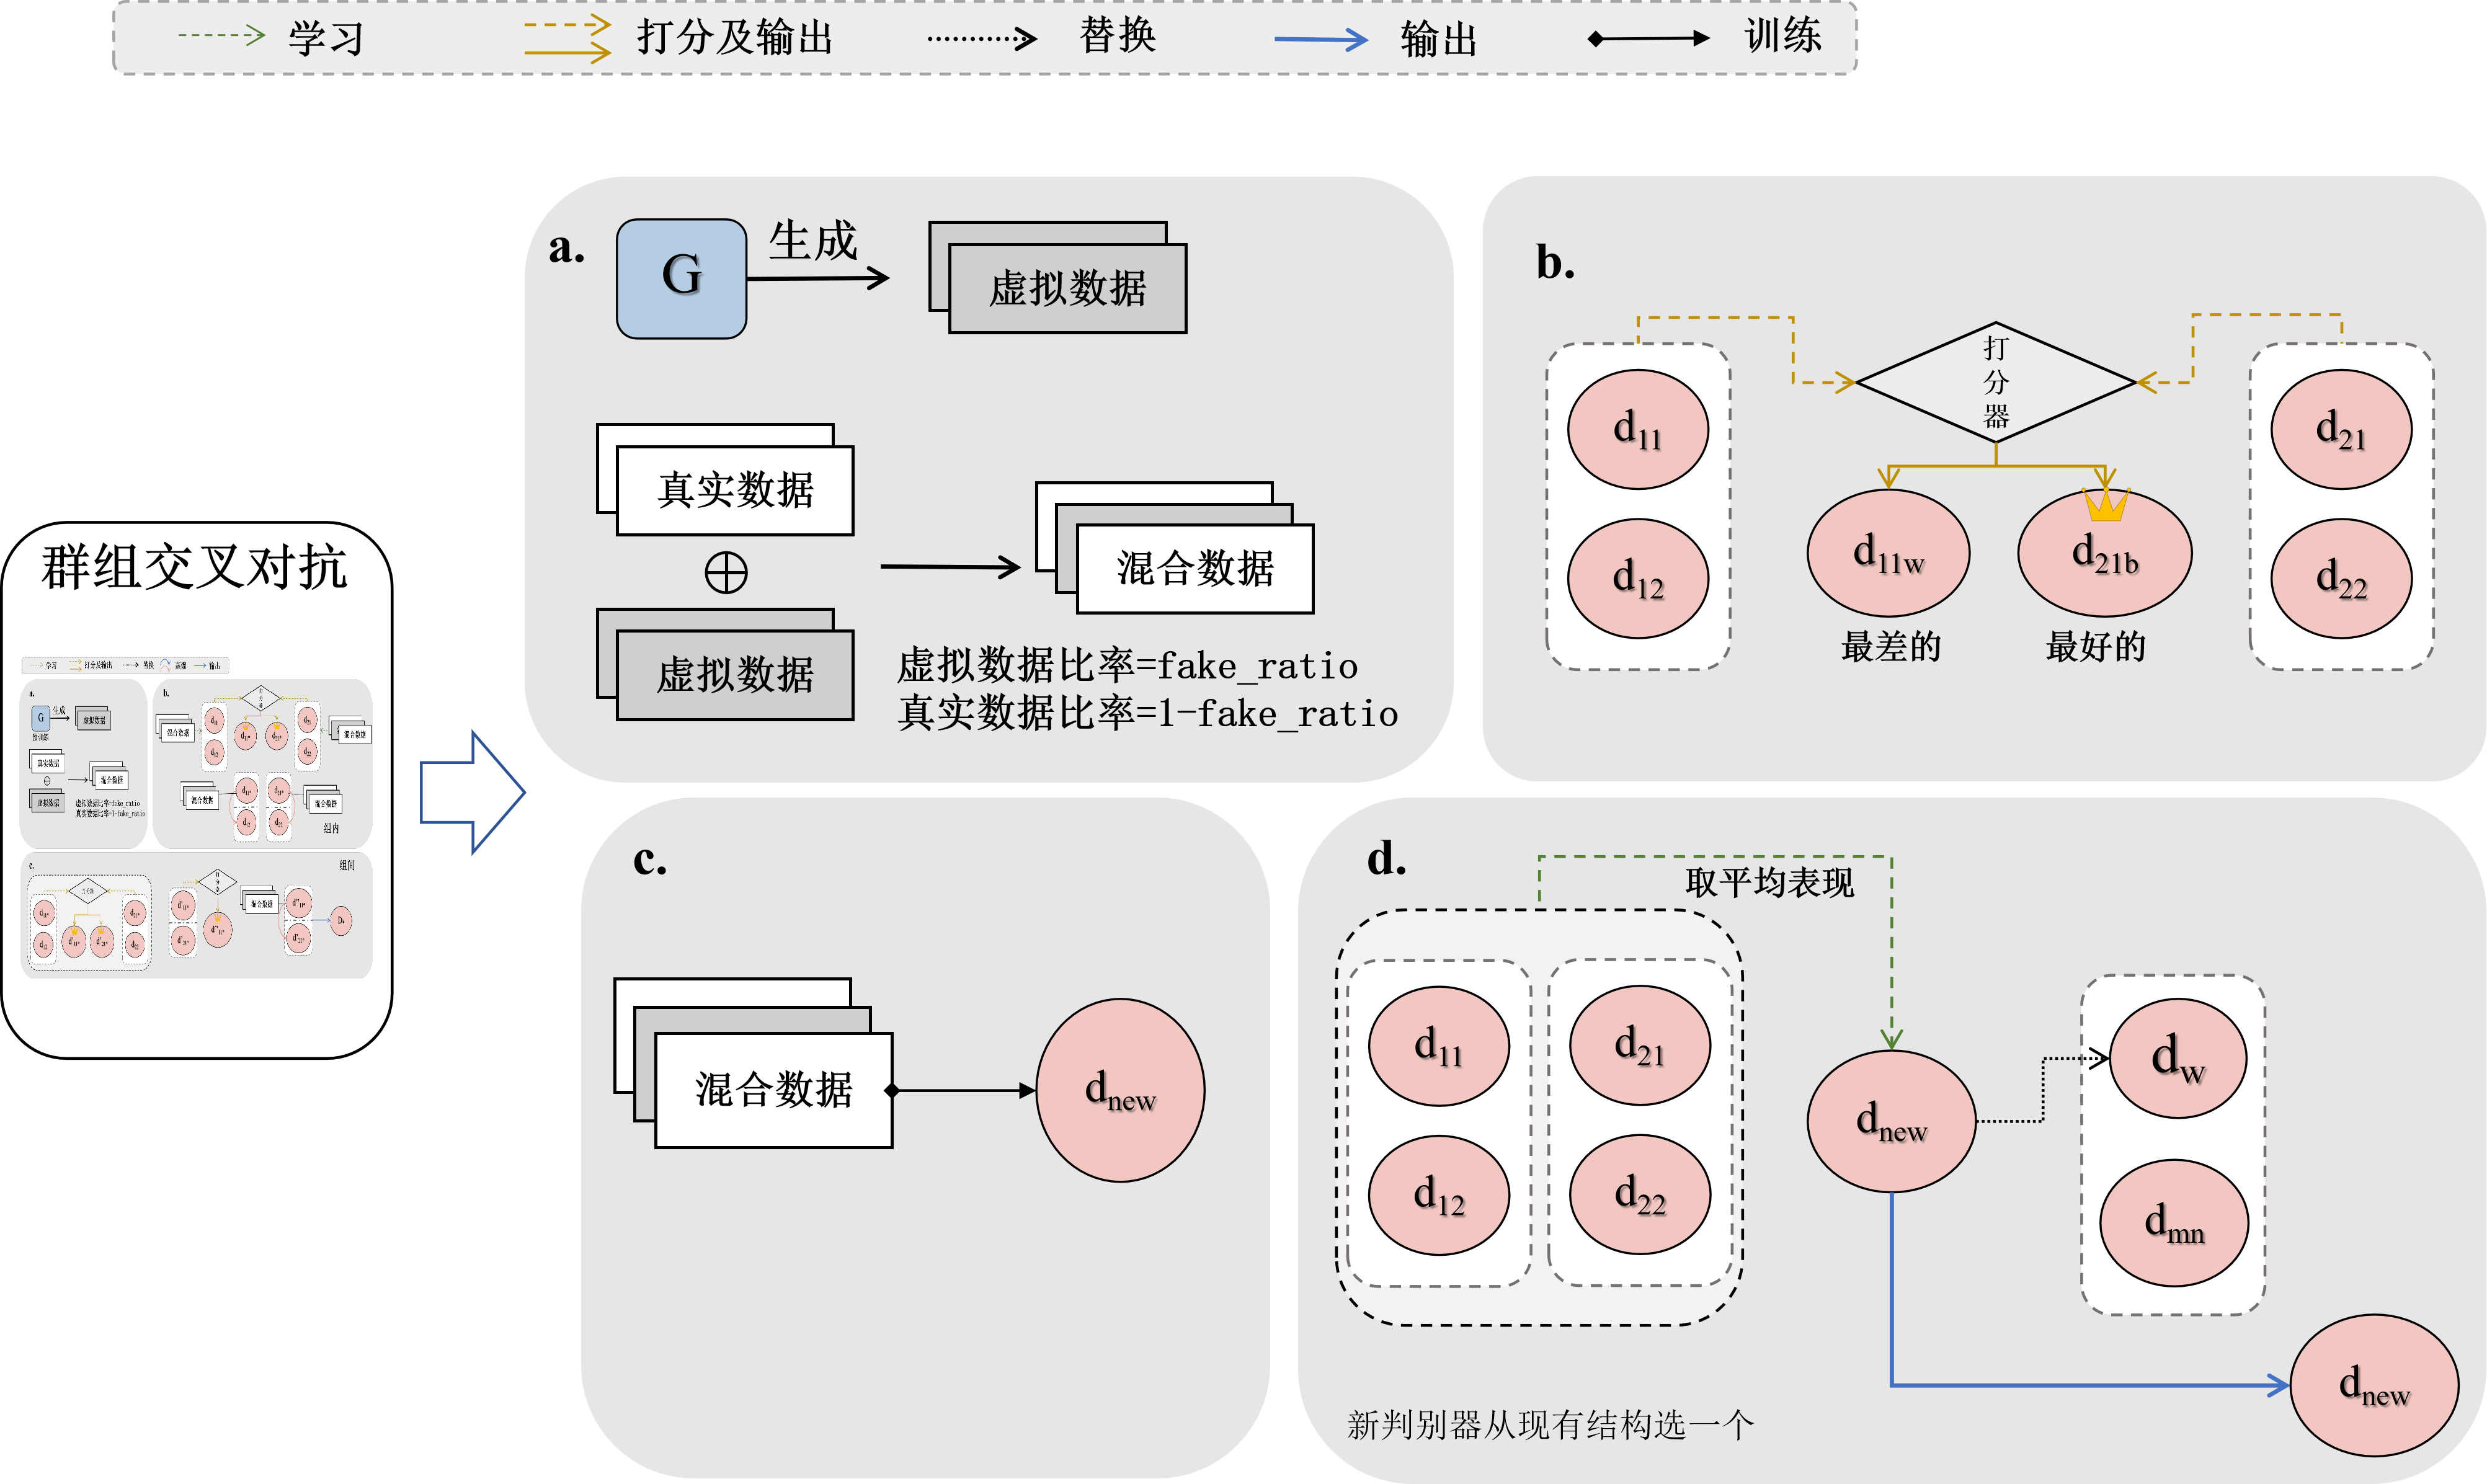
\includegraphics[width=0.8\textwidth]{figures/chap7/偏序/赛马场偏序.png}
    \caption{偏序协同对抗机制下的赛马场训练流程示意图}
    \label{fig:GCA-Partial-RT}
\end{figure}

% \begin{algorithm}
% \caption{Step 2 - Racetrack Competition (RT)}
% \label{alg:racetrack}
% \begin{algorithmic}[1]
% \State \textbf{Stage 1 \& 2: Evaluation and Targeting}
% \State Evaluate all discriminators, find $\texttt{Global\_Worst}$ and $\texttt{Global\_Best}$
% \State
% \State \textbf{Stage 3: Train New Student}
% \State Initialize $\texttt{Student\_D}$ (clone of a structure)
% \For{batch in $\texttt{Mixed\_Data}$}
%     \State $\texttt{Teacher\_Ensemble} \gets \text{Average}(\text{All\_Discriminators}(\text{batch}))$
%     \State $\text{Loss\_Student} \gets \text{CE}(\texttt{Student\_D}(\text{batch}), \text{label}) + \lambda \cdot \text{MSE}(\texttt{Student\_D}(\text{batch}), \texttt{Teacher\_Ensemble})$
%     \State Update $\texttt{Student\_D}$
% \EndFor
% \State
% \State \textbf{Stage 4 \& 5: Replacement}
% \State Replace $\texttt{Global\_Worst}$ with $\texttt{Student\_D}$
% \State Reset optimizer for the replaced position
% \State Re-evaluate and update $\texttt{Global\_Best}$
% \end{algorithmic}
% \end{algorithm}

双向师生蒸馏（S2T）阶段不仅包含常规的向最优者学习（正向蒸馏），更创新性地引入了反向蒸馏机制。系统动态监控“学生”（当前最差判别器）与“教师”（其他判别器）的性能差距。若学生在某些样本或阶段的表现超越了教师，算法会立即反转蒸馏方向，强迫教师向学生学习。这种动态的双向交互极大地丰富了模型的多样性，防止了同质化。

\begin{algorithm}[H]
\caption{双向师生蒸馏（S2T）算法流程}
\label{alg:s2t}
\begin{algorithmic}[0]
\State \textbf{阶段1：初始打分}
\State 使用打分器（验证集CE）评估每个判别器组的每个判别器
\State 找到全局CE最小的判别器 $a_1$ 和全局CE最大的判别器 $b_1$
\Statex
\State \textbf{阶段2：混合数据训练}
\State 所有判别器组中的所有判别器在赛马场阶段生成的混合数据上进行训练
\Statex
\State \textbf{阶段3：单向蒸馏}
\State 使用打分器重新评估，找到新的全局最优 $a_2$ 和全局最差 $b_2$
\For{每个判别器 $D_i$（$D_i \neq a_2$）}
    \State $\text{Loss}_{\text{Distill}} = \text{MSE}(\text{Feat}_{D_i}, \text{Feat}_{a_2}) + \text{MSE}(\text{Logits}_{D_i}, \text{Logits}_{a_2})$
    \State 使用 $\text{Loss}_{\text{Distill}}$ 更新 $D_i$，使其特征分布向 $a_2$ 靠拢
\EndFor
\Statex
\State \textbf{阶段4：组内循环评分与双向反馈}
\State 将 $b_1$ 位置的判别器定义为“学生”，其余所有判别器定义为“教师”，初始化阈值$\theta$
\For{每个教师判别器 $T_j$}
    \If{学生CE + $\theta$ < 教师CE（学生超越教师）}
        \State 反向蒸馏：强制教师 $T_j$ 拟合学生的输出与特征
    \ElsIf{教师CE + $\theta$ < 学生CE（学生落后于教师）}
        \State 正向蒸馏：强制学生拟合教师 $T_j$ 的输出与特征
    \EndIf
\EndFor
\Statex
\State \textbf{阶段5：最终评估}
\State 使用打分器评估所有判别器，找到CE最小的全局最优判别器并输出
\end{algorithmic}
\end{algorithm}

\begin{figure}[htbp]
    \centering
    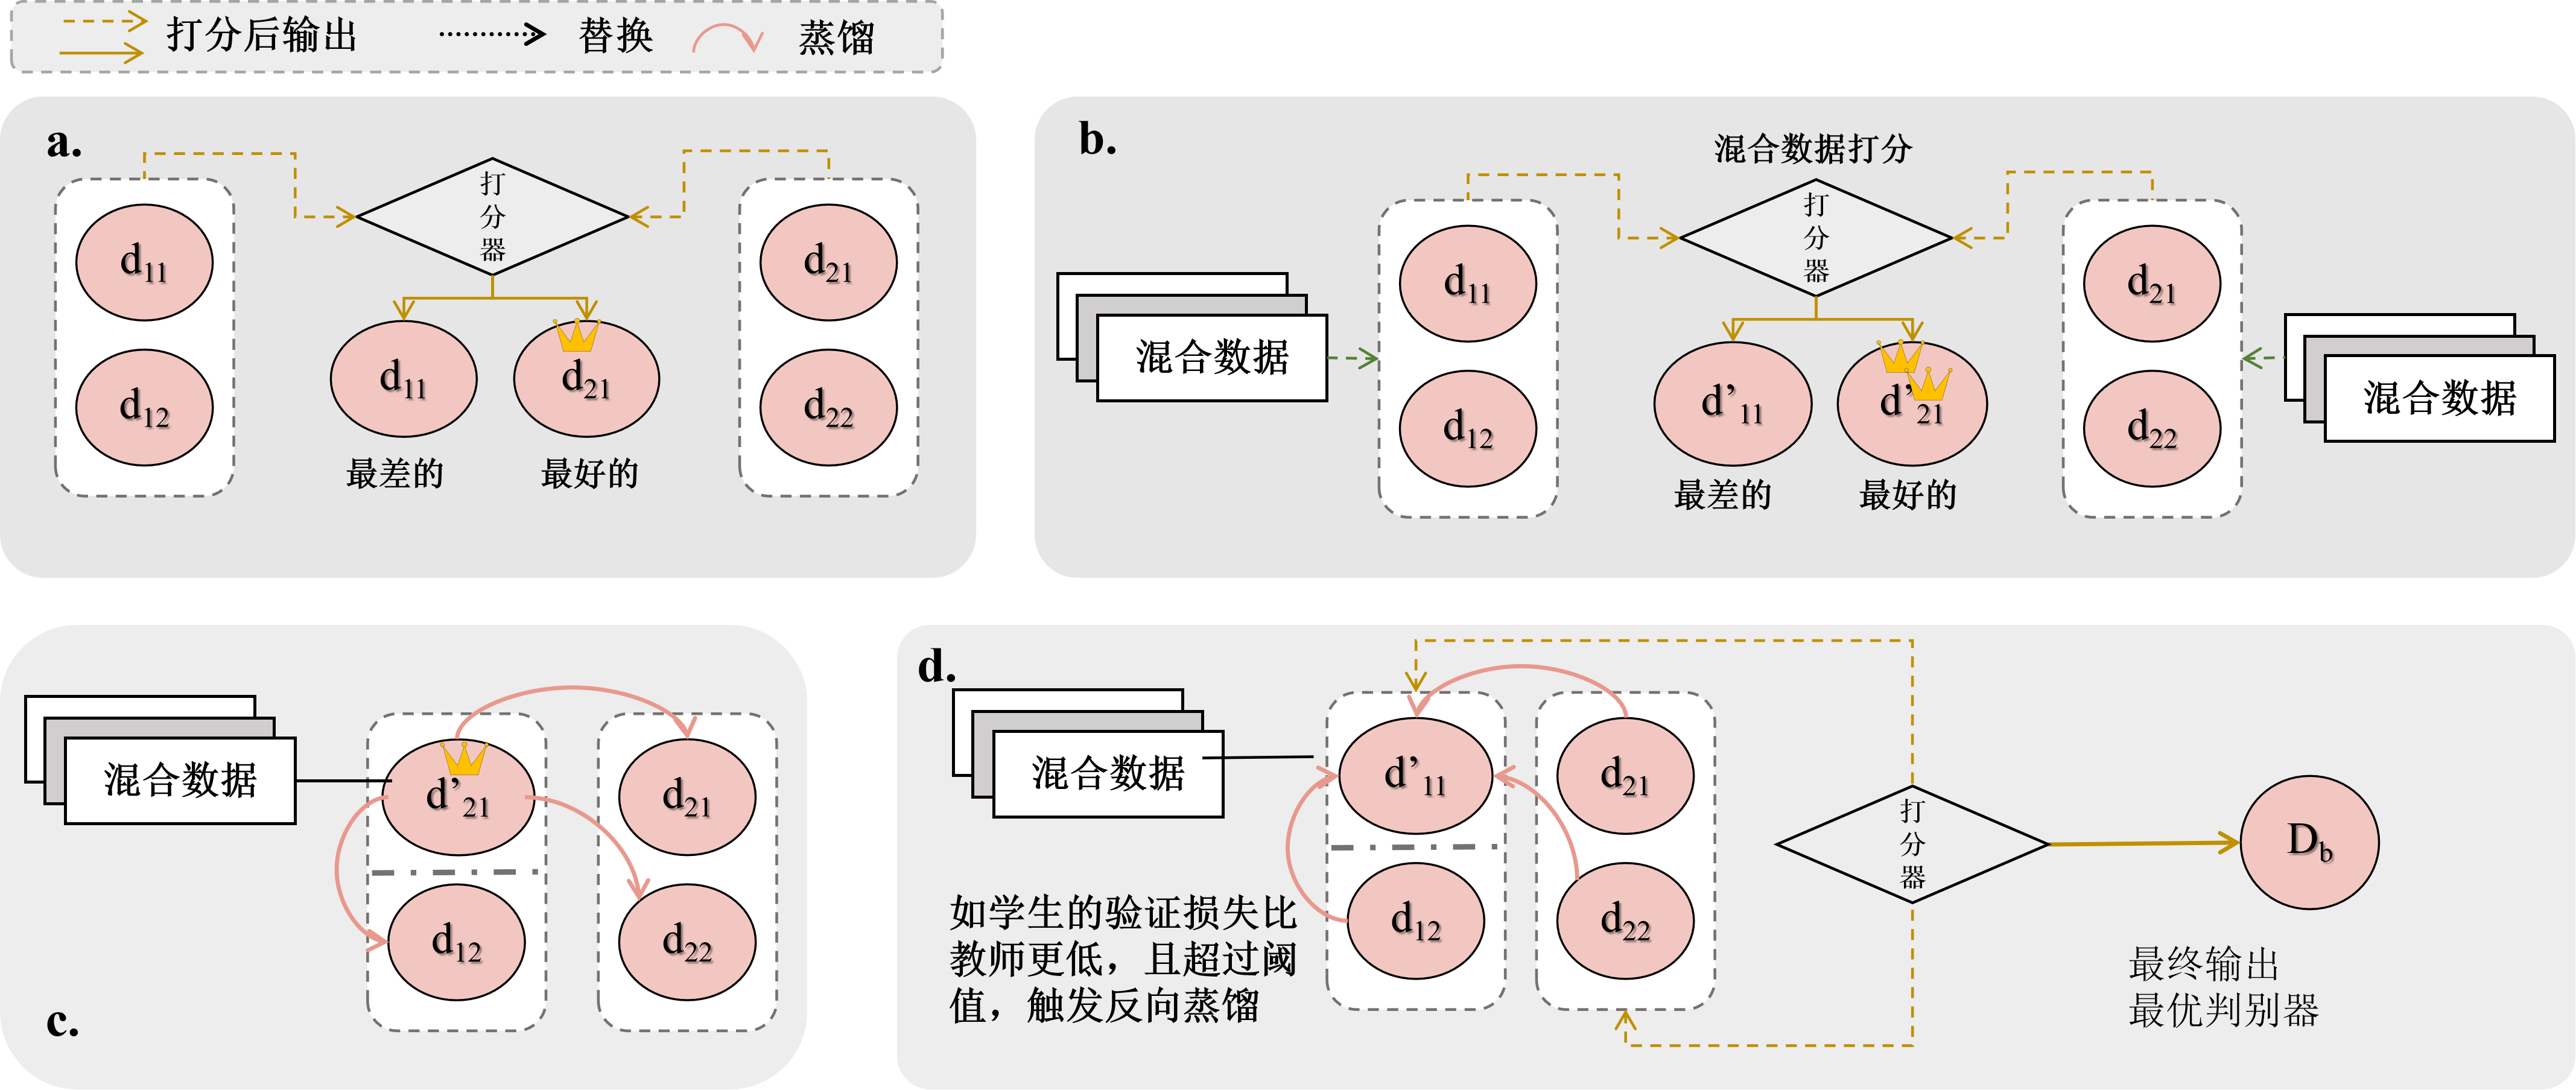
\includegraphics[width=0.8\textwidth]{figures/chap7/偏序/逆向教师偏序.png}
    \caption{偏序协同对抗机制下的逆向教师系统训练流程示意图}
    \label{fig:GCA-Partial-S2T}
\end{figure}

% \begin{algorithm}[H]
% \caption{Step 3 - Student-to-Teacher Bidirectional Distillation (S2T)}
% \label{alg:s2t}
% \textbf{Stage 1: Initial Scoring}\;
% Evaluate each discriminator in every group using the scorer (validation set CE)\;
% Identify the discriminator with the lowest global CE as $a_1$ and the highest global CE as $b_1$\;
% \BlankLine
% \textbf{Stage 2: Mixed Data Training}\;
% All discriminators in all groups train on the mixed data generated during the Racetrack stage\;
% \BlankLine
% \textbf{Stage 3: Unidirectional Distillation}\;
% Re-evaluate using the scorer, identify the new global best $a_2$ and global worst $b_2$\;
% \For{each discriminator $D_i$ ($D_i \neq a_2$)}{
%     $\text{Loss}_{\text{Distill}} = \text{MSE}(\text{Feat}_{D_i}, \text{Feat}_{a_2}) + \text{MSE}(\text{Logits}_{D_i}, \text{Logits}_{a_2})$\;
%     Update $D_i$ with $\text{Loss}_{\text{Distill}}$ to align its feature distribution toward $a_2$\;
% }
% \BlankLine
% \textbf{Stage 4: Intra-Group Cyclic Scoring with Bidirectional Feedback}\;
% Define the discriminator at position $b_1$ as the ``student'', all other discriminators as ``teachers''\;
% \For{each teacher discriminator $T_j$}{
%     \eIf{student CE $<$ teacher CE (student surpasses teacher)}{
%         Reverse distillation: force teacher $T_j$ to fit the student's output and features\;
%     }{
%         Forward distillation: force the student to fit teacher $T_j$'s output and features\;
%     }
% }
% \BlankLine
% \textbf{Stage 5: Final Evaluation}\;
% Evaluate all discriminators using the scorer, identify and output the discriminator with the lowest CE as the global best\;
% \end{algorithm}

最后，孪生对抗检测（Twin）阶段充当系统的熔断器。算法统计S2T阶段中每个判别器偏离最优判别器的程度。一旦某判别器的异常次数超过阈值，且系统中存在其他正常工作的判别器组，算法即判定该判别器失效，并使用全局最优判别器的深拷贝进行强制替换。随后，生成器与判别器进行最后一轮的高强度GAN对抗微调，确保最终输出的模型具备极高的鲁棒性。为了定量刻画智能体间的协同偏差，本章引入了 exceed\_threshold\_times（超阈值频次）作为触发参数镜像重置的核心指标，具体逻辑如下所示。

\begin{algorithm}[H]
\caption{孪生对抗检测（Twin）算法流程}
\label{alg:twin_adversarial_detection}
\begin{algorithmic}[0]
\State \textbf{异常检测}
\State 统计每个判别器相对于 \textit{Global\_Best} 的超阈值次数 \textit{exceed\_threshold\_times}
\State \textbf{条件1：}超阈值次数 $\geq$ \textit{twins\_threshold}
\State \textbf{条件2：}至少有另一个判别器组状态正常
\Statex
\State \textbf{替换与微调}
\For{每个判别器}
    \If{同时满足条件1和条件2}
        \State 使用 \textsc{DeepCopy}(\textit{Global\_Best}) 替换该判别器
        \State 重置优化器
    \EndIf
\EndFor
\Statex
\State \textbf{GAN微调}
\For{epoch $\in$ \textit{Finetune\_Epochs}}
    \State 训练 $G$：$\mathcal{L}_G = \text{Financial\_Loss} + 0.1 \times \text{Adversarial\_Loss}(D_{\text{best}})$
    \State 训练 $D_{\text{best}}$：$\mathcal{L}_D = \text{CE\_Loss}$
\EndFor
\end{algorithmic}
\end{algorithm}

\begin{figure}[htbp]
    \centering
    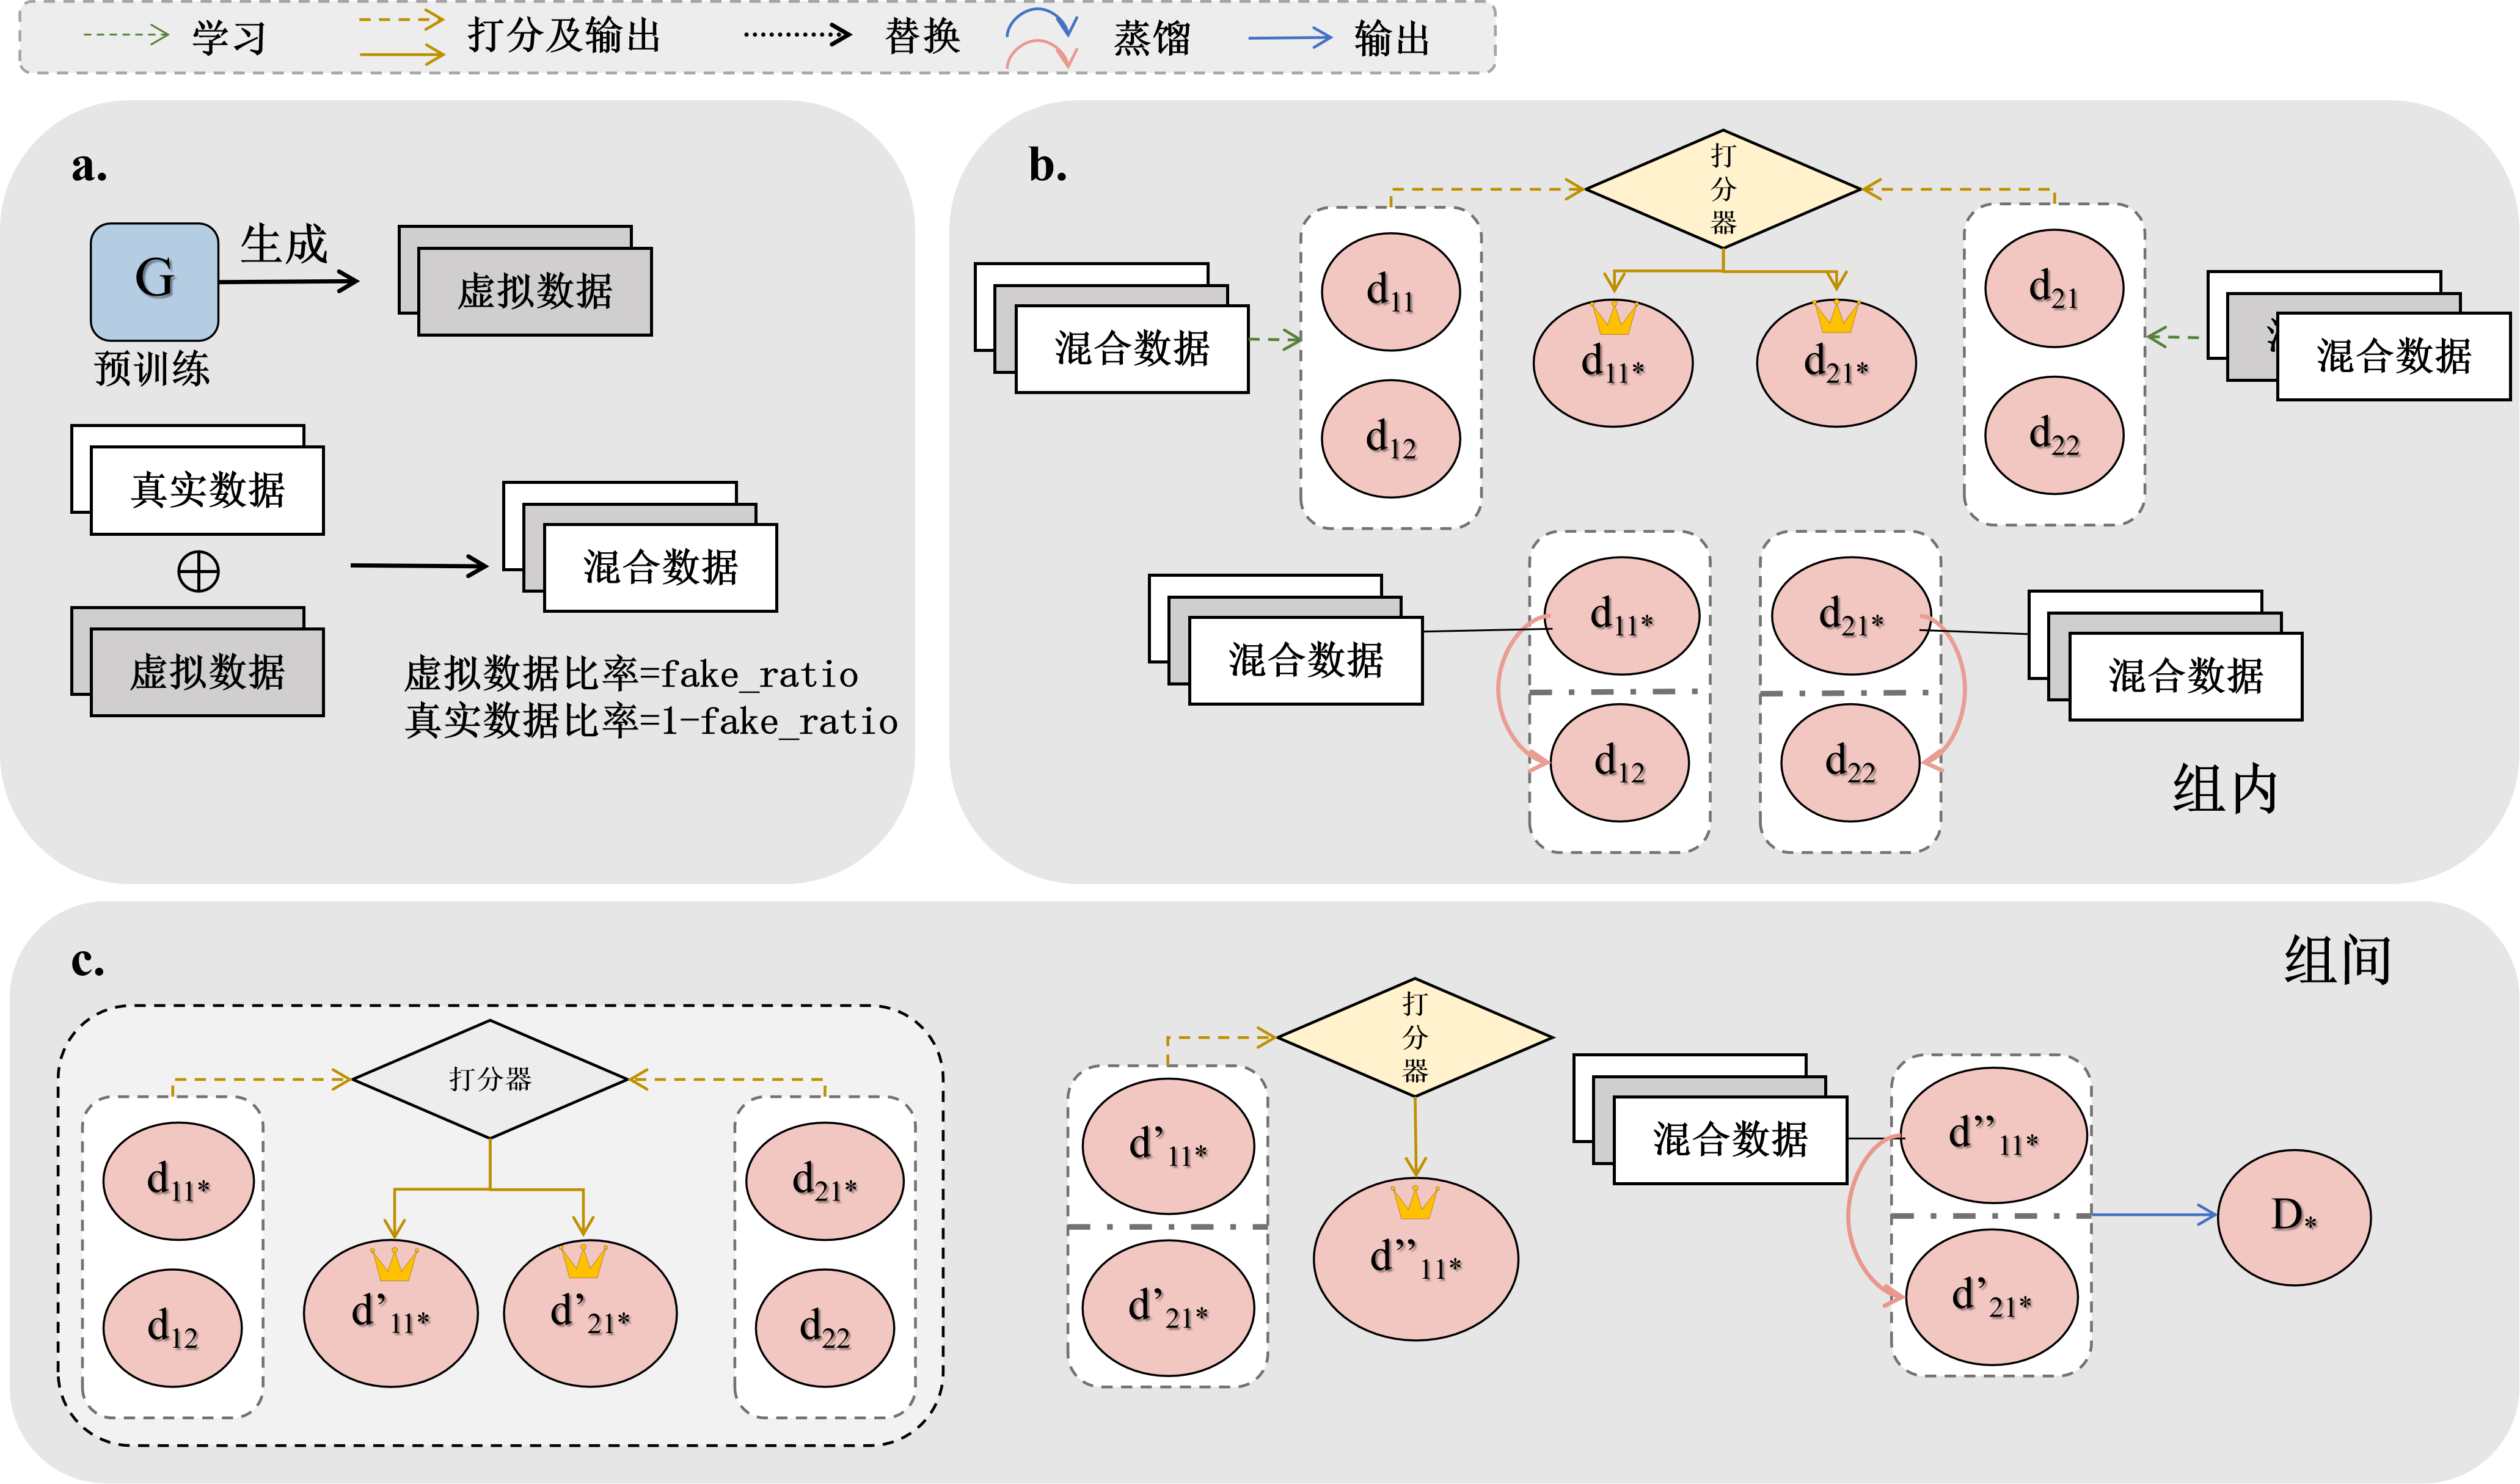
\includegraphics[width=0.8\textwidth]{figures/chap7/偏序/群组偏序.png}
    \caption{偏序协同对抗机制下的孪生对抗训练流程示意图}
    \label{fig:GCA-Partial-Twins}
\end{figure}

% \begin{algorithm}
% \caption{Step 4 - Twin Adversarial Detection}
% \label{alg:twin_adversarial_detection}
% \begin{algorithmic}[1]
% \State \textbf{Detection}
% \State Count \textit{exceed\_threshold\_times} for each discriminator relative to \textit{Global\_Best}
% \State \textbf{Condition 1:} Count $\geq$ \textit{twins\_threshold}
% \State \textbf{Condition 2:} At least one other group is normal

% \Statex
% \State \textbf{Replacement and Finetuning}
% \For{each discriminator}
%     \If{Condition 1 and Condition 2 are met}
%         \State Replace discriminator with \textsc{DeepCopy}(\textit{Global\_Best})
%         \State Reset Optimizer
%     \EndIf
% \EndFor

% \Statex
% \State \textbf{GAN Finetuning}
% \For{epoch in \textit{Finetune\_Epochs}}
%     \State Train $G$: $\mathcal{L}_G = \text{Financial\_Loss} + 0.1 \times \text{Adversarial\_Loss}(D_{\text{best}})$
%     \State Train $D_{\text{best}}$: $\mathcal{L}_D = \text{CE\_Loss}$
% \EndFor
% \end{algorithmic}
% \end{algorithm}


\subsubsection{算法复杂度分析}
设生成器数为 $N_G$（本文取1），判别器数为 $N_D$（本文取6），时间步长为 $T$，特征维度为 $F$。单轮训练中，生成器复杂度约为 $\mathcal{O}(N_G \cdot T^2 \cdot F)$，判别器前向传播复杂度为 $\mathcal{O}(N_D \cdot C_D)$；GCA 与 S2T 中的特征对齐额外引入 $\mathcal{O}(N_D^2 \cdot d_{feat})$ 开销。因此，总体时间复杂度约为 $\mathcal{O}(T^2 \cdot F + N_D \cdot C_D + N_D^2 \cdot d_{feat})$。由于 $N_D=6$，新增协同计算开销仍处于可接受范围。

\section{实验}
本节将对偏序协同对抗架构在涨跌分类任务中的有效性进行全面的实验验证。首先介绍实验设计与评估体系，随后详细分析数据集特征、模型分类性能及各创新点的独立贡献。

\subsection{实验设计与评估体系}
本章实验逻辑延续了前文的评价体系，并在更复杂的涨跌分类任务下验证了前述偏序结构的普适性。

\subsubsection{训练配置与优化策略}
实验在 PyTorch 框架下完成。生成器与判别器均采用 Adam 优化器，学习率分别设为 $4\times10^{-5}$ 和 $2\times10^{-5}$，Betas 为 $(0.9, 0.999)$，批量大小为64，初始训练轮数为100。为抑制过拟合和梯度不稳定，训练中同时采用最大范数为1.0的梯度裁剪与 0.1 的 Dropout。

\begin{figure}[h]
\label{fig:Partialorderadversarialarchitecture}
\centering
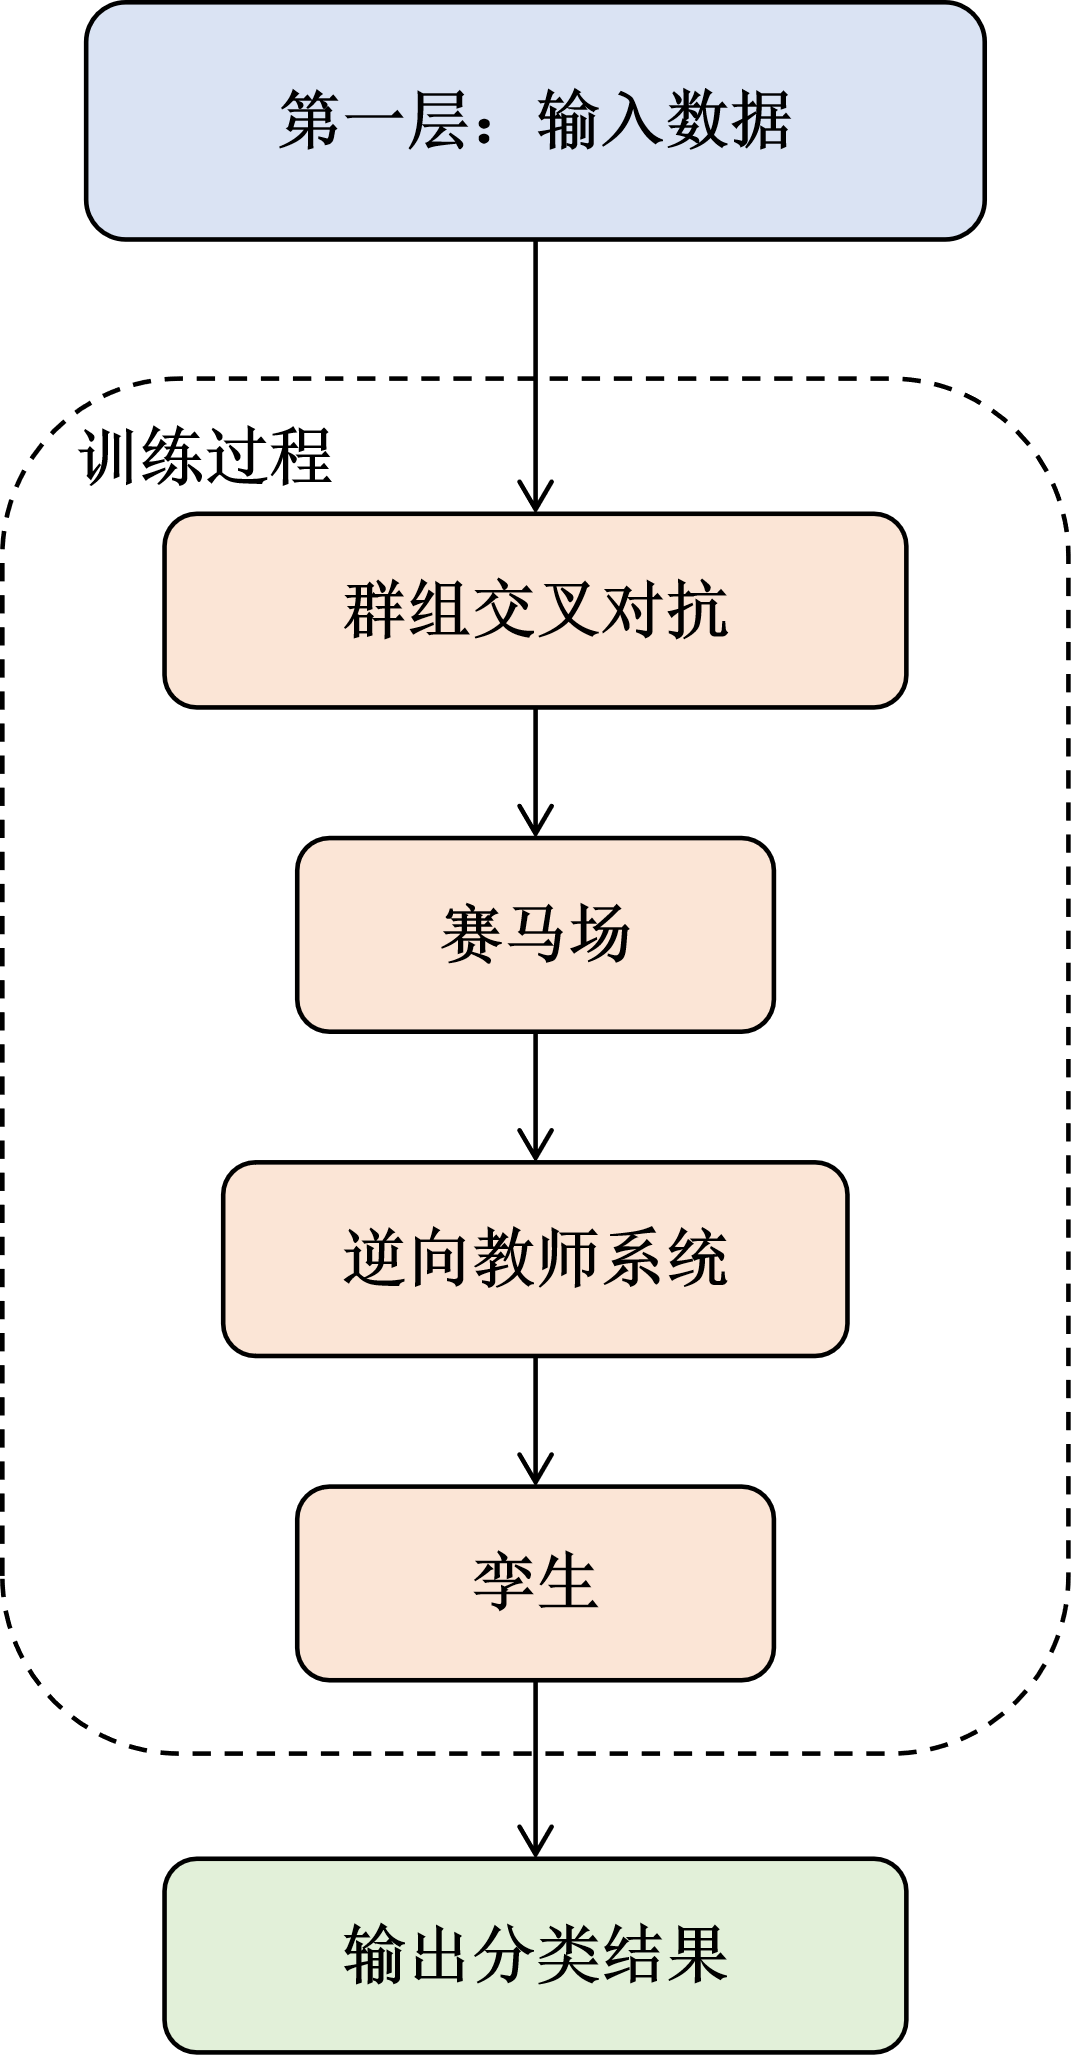
\includegraphics[width=0.5\textwidth]{figures/chap7/偏序/偏序架构.png}
\caption{偏序协同对抗架构图}
\end{figure}

\subsubsection{评估指标体系}
为全面评估 MGCA，本章构建了涵盖价格预测、判别器分类、VWAP 回测与成交量预测的综合指标体系。价格层面采用 MSE、RMSE、MAE、方向准确率和 $R^2$；判别器层面采用 CE Loss、Accuracy 与 AUC；交易层面重点考察买卖信号准确率、胜率、夏普比率、VWAP Power、滑点与成本节省；成交量层面则使用 RMSE、MAE 与相关系数。该体系既衡量统计表现，也强调实际交易价值。

\subsubsection{回测框架与评估指标}
本章的交易回测以 MGCA 框架判别器输出的涨跌分类信号为基础，通过预设的信号生成规则将分类预测转换为交易指令（买入、卖出、持有），并以每笔交易的单期收益率作为核心绩效衡量指标。

具体而言，回测过程不引入保证金制度或账户复利，仅统计每笔完整交易的价格变化率。设入场价格为 $P_{\text{entry}}$，出场价格为 $P_{\text{exit}}$，则单笔交易收益率为：
\begin{equation}
r_{\text{trade}} = \frac{P_{\text{exit}} - P_{\text{entry}}}{P_{\text{entry}}}.
\end{equation}
基于 $N$ 笔交易的收益率序列 $\{r_1, r_2, \dots, r_N\}$，各评估指标计算方式如下：
\begin{itemize}
    \item \textbf{平均收益率} $\bar r = \frac{1}{N}\sum_{i=1}^{N} r_i$：所有交易笔收益率的算术平均值，反映策略的单笔平均盈利能力。该指标为原始比例（非百分比），不代表年化复利收益。
    \item \textbf{胜率} $\text{WinRate} = \frac{\#\{r_i > 0\}}{N}$：盈利交易笔数占总交易笔数的比例。
    \item \textbf{夏普比率} $\text{Sharpe} = \frac{\bar r}{\sigma_r} \cdot \sqrt{252}$：其中 $\sigma_r$ 为交易收益率的标准差，$\sqrt{252}$ 为年化因子（隐含日频交易假设）。当交易笔数少于 2 或 $\sigma_r$ 过小时，夏普比率设为 0。
\end{itemize}
需要说明的是，文中“年化收益率”仅为 $\bar r \times 252$ 的参照表达，并非账户实际复利收益。

\subsubsection{数据集与筛选标准}
实验涵盖19个中国期货合约，覆盖股指、贵金属、基础金属、能源、农产品等类别，所有实验均在生成器学习率 $4\times10^{-5}$ 的统一设置下进行。为保证统计可靠性，交易性能分析仅保留交易次数不少于5笔的配置。

\subsubsection{实验配置与创新点组合策略}
MGCA 采用模块化设计，偏序协同架构为基础配置，RT、S2T 与 Twin 可灵活组合。配置代码中，第一位表示是否启用偏序协同架构，后两位分别表示 RT 和 S2T；Baseline 则为不含偏序协同架构的传统单生成器单判别器模式。通过逐步叠加模块，可识别架构本身及各创新点的增量贡献。

\subsubsection{软硬件环境}
实验平台配备 NVIDIA GeForce RTX 3090 GPU（24GB 显存）、Intel Core i9-10900K CPU 和 64GB DDR4 内存，软件环境为 Ubuntu 20.04 LTS 与 PyTorch，数据处理主要依赖 Pandas、NumPy 和 Scikit-learn。

\subsubsection{随机性控制与参数初始化}
考虑到 GAN 训练的敏感性，实验统一设置全局随机种子，采用 Xavier Uniform 初始化，并通过可视化工具监控损失曲线、梯度范数和验证集 MSE。训练中使用早停机制：若验证集 MSE 连续10个 epoch 未下降，则终止训练并回滚到最优权重，同时定期保存中间检查点以支持后续分析。下面进一步对19个期货合约的数据特征进行分析。

\subsection{数据集特征与市场特征分析}


为了全面理解MGCA框架的性能表现，我们首先分析了19个期货合约的原始数据特征和市场特征。每个合约包含830个每日数据点，涉及7大资产类别，展现出不同的市场特征。表\ref{tab:assetstatssideways}展示了各资产类别的原始数据特征统计，本次统计采用标准的金融时间序列分析方法，收益率的计算公式为：每日收益率 = (当日收盘价 - 前日收盘价) / 前日收盘价 × 100\%。统计指标包括均值、标准差、最小值和最大值、偏度和峰度。所有19个合约的数据点数均为830个交易日，时间跨度完全一致，确保了跨资产类别比较的有效性。

\begin{table}[htbp]
\centering
\caption{资产类别统计特征}
\label{tab:assetstatssideways}
\scriptsize
\setlength{\tabcolsep}{2pt}
\renewcommand{\arraystretch}{1.5}
\resizebox{\textwidth}{!}{%
\begin{tabular}{@{}lcccccccc@{}}
\toprule
\textbf{资产类别} & \textbf{合约数} & \textbf{数据点数} & \textbf{平均收益率(\%)} & \textbf{收益率标准差(\%)} & \textbf{收益率范围} & \textbf{平均偏度} & \textbf{平均峰度} & \textbf{市场特征} \\
\midrule
国债     & 1 & 830 & 0.0096 & 0.1704 & $-0.91\%$ 到 $0.67\%$ & -0.62 & 2.86 & 接近零收益、低波动、负偏度 \\
贵金属   & 2 & 830 & 0.0895 & 1.1572 & $-8.07\%$ 到 $7.35\%$ & -0.31 & 4.12 & 正收益、中等波动、负偏度 \\
股指     & 2 & 830 & -0.0194 & 1.2263 & $-10.02\%$ 到 $8.69\%$ & 0.12 & 10.11 & 负收益、中等波动、高峰度 \\
基础金属 & 2 & 830 & 0.0113 & 1.7258 & $-17.00\%$ 到 $17.00\%$ & 0.01 & 7.73 & 正收益、高波动 \\
能源     & 2 & 830 & 0.0105 & 2.2318 & $-13.18\%$ 到 $25.58\%$ & 1.38 & 16.27 & 正收益、极高波动、正偏度、高峰度 \\
农产品   & 7 & 830 & -0.0151 & 1.4126 & $-17.03\%$ 到 $7.91\%$ & -0.71 & 8.37 & 负收益、中等波动、负偏度 \\
工业品   & 3 & 830 & -0.0013 & 1.7733 & $-11.99\%$ 到 $9.53\%$ & -0.12 & 2.53 & 接近零收益、高波动 \\
\bottomrule
\end{tabular}%
}
\end{table}

国债类别以十年债T为代表，展现出金融市场中最稳定的特征，其收益率标准差仅为0.1704\%，是所有资产类别中波动性最低的，收益率分布呈现负偏度特征（-0.62），表明极端下跌事件相对更频繁，但整体波动幅度极小，峰度为2.86接近正态分布，这种低波动性特征使得MGCA判别器在该合约上能够更准确地捕捉价格模式。

贵金属类别包含沪金au和沪银ag两个合约，平均收益率为0.0895\%，显著高于其他资产类别，收益率标准差为1.1572\%，属于中等波动水平，负偏度（-0.31）表明价格下跌时波动相对更大，峰度4.12略高于正态分布，说明存在一定的极端价格波动，这种特征使得贵金属既具有投资价值又保持相对稳定。

股指类别包含沪深300IF和上证50IH两个合约，平均收益率为负值（-0.0194\%），反映了统计期间股指市场的整体下行趋势，但其最显著的特征是高峰度（10.11），远超正态分布的3，表明股指市场存在频繁的极端价格波动事件，这种高峰度特征与MGCA框架中S2T和RT创新点的高峰值性能表现形成了有趣的对应关系。

基础金属类别包含铜cu和镍ni两个合约，平均收益率为正（0.0113\%），收益率标准差达到1.7258\%，属于高波动类别，收益率范围从-17.00\%到17.00\%，展现出基础金属市场的剧烈波动特性，偏度接近零（0.01）表明分布相对对称，峰度7.73说明极端事件较为常见。

能源类别包含原油sc和液化石油气pg两个合约，是所有资产类别中波动性最高的，收益率标准差达到2.2318\%，收益率范围从-13.18\%到25.58\%，特别是液化石油气pg展现出极端的正偏度（2.96）和高峰度（29.21），表明该合约存在罕见的极端上涨事件，这种极高波动性对MGCA框架提出了严峻挑战，但实验结果显示MGCA仍然成功实现了从负收益到正收益的转变。

农产品类别包含7个合约（棉花CF、苹果AP、玉米c、豆粕m、豆油y、菜籽油OI、尿素UR），是合约数量最多的类别，平均收益率为负值（-0.0151\%），收益率标准差为1.4126\%属于中等波动，负偏度（-0.71）表明价格下跌时波动更大，峰度8.37说明存在较多的极端价格事件，这种负收益和负偏度特征反映了农产品市场在统计期间的整体疲软。

工业品类别包含3个合约（螺纹钢rb、铁矿石i、对苯二甲酸PTA），平均收益率接近零（-0.0013\%），收益率标准差为1.7733\%属于高波动类别，偏度接近零（-0.12）表明分布相对对称，峰度2.53接近正态分布，这种高波动但分布相对正态的特征使得工业品市场既充满交易机会又保持一定的可预测性。


在完成基础统计后，本节进一步通过可视化手段深入剖析数据特征的分布规律。



\begin{figure}[htbp]
\centering

\includegraphics[width=0.8\textwidth]{figures/chap7/偏序/收益率分布对比_按资产类别.png}
\caption{各资产类别收益率分布对比}
\label{fig:data_return_distribution}
\end{figure}

图\ref{fig:data_return_distribution}通过六个子图展示了19个期货合约在七大资产类别上的日收益率概率密度分布特征，基于830个交易日的每日收盘价数据计算得出。

国债类别（十年债T）展现出最集中的分布形态，收益率主要集中在-0.5\%到0.5\%的狭窄区间内，标准差仅为0.17\%，反映了国债市场的极低波动性和高度稳定性。贵金属类别（沪金au、沪银ag）呈现中等波动水平，分布较为对称但略带负偏，收益率范围为-8\%到7\%，平均波动率1.16\%。股指类别（沪深300IF、上证50IH）具有显著的高峰度特征（平均峰度10.11），分布呈现明显的长尾现象，极端收益率事件（单日涨跌幅超过8\%）的发生频率远高于正态分布的预期，这是股票市场“肥尾”特征的典型表现。基础金属类别（铜cu、镍ni）和能源类别（原油sc、液化石油气pg）展现出最高的波动性，分布极度分散，能源类别的平均波动率达2.23\%，收益率范围从-13\%到+26\%，反映了能源市场受供需关系、地缘政治等多重因素影响的剧烈价格波动特性。农产品类别（7个合约）和工业品类别（3个合约）的分布形态介于上述极端情况之间，呈现中等波动水平和较为对称的分布特征。这些分布特征的差异直接反映了不同资产类别的市场结构、交易机制和风险特征的本质差异。

\begin{figure}[htbp]
\centering

\includegraphics[width=0.8\textwidth]{figures/chap7/偏序/波动率对比_各合约.png}
\caption{各合约波动率对比}
\label{fig:volatilitycomparison}
\end{figure}

图\ref{fig:volatilitycomparison}以横向柱状图的形式展示了19个期货合约的波动率排名，波动率以日收益率的标准差衡量，并通过颜色编码区分不同资产类别。

波动率排名呈现显著的分层结构：最高波动率组由镍ni（2.42\%）、铁矿石i（2.31\%）、原油sc（2.30\%）和液化石油气pg（2.17\%）组成，这四个合约均属于基础金属和能源类别，反映了这些大宗商品市场受全球供需关系、宏观经济和地缘政治因素影响的剧烈波动特性。中等波动率组包括农产品和工业品合约，波动率在1.2\%-1.9\%范围内，如尿素UR(1.92\%）、苹果AP（1.64\%）等。最低波动率组由十年债T（0.17\%）领衔，其波动率仅为最高波动率合约的1/14，充分体现了国债作为无风险资产的稳定性特征。其次是玉米c（0.75\%）、沪金au（0.81\%）和铜cu（1.03\%），这些合约的低波动性与其市场成熟度、流动性和价格发现机制的完善程度密切相关。这种波动率的巨大差异说明了不同资产类别在风险特征上的本质区别，也为投资组合的风险分散和资产配置提供了重要参考。

\begin{figure}[htbp]
\centering

\includegraphics[width=0.8\textwidth]{figures/chap7/偏序/偏度峰度散点图.png}
\caption{各合约偏度峰度散点图}
\label{fig:skewnesskurtosis}
\end{figure}

图\ref{fig:skewnesskurtosis}以散点图的形式展示了19个期货合约在偏度-峰度二维平面上的分布特征，揭示了收益率分布的对称性和尾部厚度特征。图中最显著的离群点是液化石油气pg，其偏度高达2.96、峰度高达29.21，远超其他所有合约，表明该合约存在极端的右尾分布特征，即极端上涨事件（单日涨幅超过25\%）的发生频率远高于正态分布的预期，这与能源市场的突发性供给冲击特征高度契合。第二梯队的高峰度合约包括豆粕m（峰度22.42）、苹果AP（峰度16.82）和沪深300IF股指期货（峰度11.80），这些合约的高峰度特征说明其收益率分布具有显著的“肥尾”现象，极端价格波动事件的发生频率较高。在偏度维度上，大多数合约集中在偏度-0.5到0.5的范围内，表明分布相对对称，但存在显著例外：豆粕m的偏度为-2.36，苹果AP的偏度为-1.36，表明这些农产品合约存在显著的左尾分布特征，极端下跌事件的概率较高，这可能与农产品市场的季节性供给冲击和需求疲软有关。国债十年债T位于图的左下角（偏度-0.62、峰度2.86），其低峰度特征表明分布接近正态，极端事件罕见，这与国债市场的稳定性特征高度一致。该图还显示了资产类别之间的系统性差异：能源和农产品合约倾向于高峰度，股指合约也具有高峰度特征，而国债和部分工业品合约则表现出相对正态的分布特征。

\begin{figure}[htbp]
\centering

\includegraphics[width=0.8\textwidth]{figures/chap7/偏序/收益率箱线图_按资产类别.png}
\caption{各资产类别收益率分布箱线图}
\label{fig:returnsboxplot}
\end{figure}

图\ref{fig:returnsboxplot}以箱线图的形式系统性地展示了七大资产类别的收益率分布特征，包括中位数、四分位数范围、离群值和极端值等关键统计量。国债类别展现出最窄的箱体，箱体高度（25\%-75\%分位数范围）仅约0.3\%左右，须线范围（1.5倍IQR）也仅为-0.9\%到0.7\%，几乎没有离群值，这充分体现了国债市场的极低波动性和高度集中的分布特征。贵金属类别的箱体高度约1.5\%，中位数略高于零，显示出温和的正收益特征，但存在一些负向离群值（最低达-8\%），表明偶尔会出现较大幅度的价格回调。股指类别的箱体中位数略低于零，与其负平均收益率（-0.019\%）一致，但最显著的特征是存在大量的正负向离群值，最大正向离群值达+8.7\%、最大负向离群值达-10\%，这些离群值对应于股市的暑涨暑跌事件，验证了股指市场的高峰度特征。能源类别展现出最宽的箱体（高度约3\%）和最多的正向离群值，特别是存在一个极端离群值达+25.6\%（对应液化石油气pg的极端上涨事件），这是所有资产类别中最大的单日涨幅，充分说明了能源市场的极端波动性和突发性供给冲击特征。农产品类别的箱体中位数略低于零，与其负平均收益率（-0.015\%）一致，箱体高度约2\%，存在较多的负向离群值（最低达-17\%），这与农产品市场的负偏度特征（-0.71）高度一致，说明农产品价格下跌时的波动幅度往往更大。工业品类别的箱体中位数接近零，箱体高度约2.5\%，分布相对对称，但存在一些正负向离群值（范围-12\%到+9.5\%），反映了工业品市场在整体稳定的同时也会受到周期性经济波动的影响。通过对比七大资产类别的箱线图，可以清晰地看到不同市场的风险-收益特征：国债低风险低收益、能源高风险高波动、股指高峰度高不确定性、农产品负偏度下行风险，这些特征差异为不同风险偏好的投资者提供了多样化的选择。


在深入理解数据集特征的基础上，本小节将核心焦点转向模型性能的评估，首先对比偏序协同架构与传统Baseline模型在判别器分类任务上的表现差异。

\subsection{模型整体性能与趋势捕捉能力分析}

在展开详细分析之前，有必要明确本章涉及的三个关键对比基准的定义及其架构差异：

\begin{itemize}
\item \textbf{Baseline}：传统单模型架构，由1个生成器和1个判别器组成，使用独立的标准对抗训练流程（\texttt{train\_baseline\_model}），不涉及MGCA框架的任何组件。每个合约运行4种Baseline配置：Baseline-CNN-Direct、Baseline-CNN-VAE、Baseline-Transformer-Direct、Baseline-Transformer-VAE，其中判别器类型（CNN或Transformer）由配置名称显式指定，生成器类型从GRU、LSTM、Transformer三种架构中选取（具体类型因进程级随机种子而异，实验输出中未记录），成交量预测方法（Direct或VAE）决定VWAP执行时的成交量来源。对比时选取每个合约上表现最优的Baseline配置。
\item \textbf{MGCA-000}：采用单生成器（Transformer）+单判别器（CNN）的架构，通过MGCA框架的训练流程（\texttt{train\_single\_experiment}）进行训练，三个创新点全部关闭（GCA=0, RT=0, S2T=0）。MGCA-000与Baseline的区别体现在两个层面：（1）模型类型固定——MGCA-000的生成器始终为Transformer（代码中\texttt{gen\_types[0]}）、判别器始终为CNN（代码中\texttt{disc\_types[0]}），而Baseline有CNN和Transformer两种判别器变体；（2）训练流程不同——MGCA-000使用MGCA框架的基础训练管线（包括预训练阶段等），而Baseline使用独立的标准训练流程。MGCA-000作为MGCA框架内部的基线对照，用于分离框架训练流程本身与创新点各自的贡献。
\item \textbf{偏序协同架构（配置100）}：采用MGCA多组多成员架构（1组Transformer生成器 + 2组判别器，每组3个成员，判别器类型为CNN和Transformer交替），开启群组交叉对抗训练（GCA=1, RT=0, S2T=0）。偏序协同架构与MGCA-000的区别在于两个层面：（1）架构层面——从单判别器扩展为2组$\times$3个共6个判别器的多组多成员架构；（2）训练机制层面——偏序协同架构引入了四阶段偏序协同对抗训练流程（生成器预训练$\to$生成混合数据$\to$组内对抗$\to$组间对抗），使判别器通过多样化的交叉对抗获得更强的判别能力。
\end{itemize}

上述配置名称中的Direct/VAE后缀指VWAP执行模拟时的成交量预测方法，不影响生成器和判别器的对抗训练过程本身：
\begin{itemize}
\item \textbf{Direct}：VWAP执行时直接使用生成器输出的第5维（Volume维度）作为成交量预测，即生成器在预测OHLCV五维序列的同时完成成交量预测，无需额外模型。
\item \textbf{VAE}：VWAP执行时使用独立训练的TransformerVAE pipeline进行成交量预测。该pipeline包含5个阶段：（1）加载OHLCV数据；（2）训练TransformerVAE（t分布先验）学习潜在表示；（3）生成潜在特征；（4）训练LatentOHLCVPredictor预测未来潜在特征；（5）通过VAE解码器还原为OHLCV空间并提取成交量预测。VAE方法通过潜在空间的低维表示和概率建模，旨在提升成交量预测的鲁棒性。
\end{itemize}

因此，偏序协同架构相对于Baseline的性能差异包含了三个层面的贡献：（1）MGCA训练流程本身的优化效应；（2）多组多成员架构的集成效应；（3）偏序协同对抗训练机制的创新点贡献。后续“偏序协同架构创新点贡献度分析“小节将通过偏序协同架构与MGCA-000的对比，分离出第（2）和（3）项的联合贡献。

需要说明的是，判别器AUC指标衡量的是MGCA框架内部判别器区分真实样本与生成样本的能力，该指标仅在多组多成员架构中计算。Baseline实验采用单判别器架构且使用独立的训练流程，不产生可比的判别器AUC数据，因此判别器AUC的对比基准为理论随机分类器（AUC=0.5）。

基于228个有效判别器配置的性能分析，我们验证偏序协同架构（配置100）的判别器性能。偏序协同架构（配置100）的平均AUC为0.5907，相比随机分类器基准0.5000提升18.13\%，最高AUC达0.8985，充分证明了偏序协同架构判别器在区分真实与生成样本方面的有效性。

\begin{table}[htbp]
\centering
\caption{偏序协同架构对判别器AUC性能的影响分析}
\label{tab:aucPerformanceGCA}
\scriptsize
\setlength{\tabcolsep}{2pt}
\resizebox{\textwidth}{!}{%
\begin{tabular}{ccccccccccc}
\toprule
\textbf{配置} & \textbf{配置代码} & \textbf{随机基准AUC} & \textbf{配置平均AUC} & \textbf{相对提升} & \textbf{中位数AUC} & \textbf{标准差} & \textbf{最高AUC} & \textbf{判别器数} & \textbf{最佳合约} & \textbf{最佳合约AUC} \\
\midrule
偏序协同架构 & 100 & 0.5000 & 0.5907 & +18.13\% & 0.5720 & 0.0792 & 0.8985 & 228 & 十年债T & 0.7964 \\
\bottomrule
\end{tabular}%
}
\end{table}

\begin{table}[htbp]
\centering
\caption{偏序协同架构对判别器AUC性能的多维度分析}
\label{tab:aucPerformanceMultidimplusGCA}
\scriptsize
\setlength{\tabcolsep}{4pt}
\begin{tabular}{lcccccccc}
\toprule
\textbf{配置} & \textbf{代码} & \textbf{均值} & \textbf{中位数} & \textbf{最小} & \textbf{最大} & \textbf{标准差} & \textbf{CV(\%)} & \textbf{准确率} \\
\midrule
偏序协同架构 & 100 & 0.5907 & 0.5720 & 0.4970 & 0.8985 & 0.0792 & 13.40 & 77.04\% \\
\bottomrule
\end{tabular}
\end{table}

表\ref{tab:aucPerformanceGCA}和表\ref{tab:aucPerformanceMultidimplusGCA}系统性地展示了偏序协同架构在判别器性能上的多维度表现，基于19个期货合约的228个判别器配置的真实测试集数据。偏序协同架构的平均AUC为0.5907，显著优于随机分类器的理论基准值0.5000，相对提升达18.13\%，充分证明了偏序协同架构在二分类任务上的有效性。

中位数AUC（0.5720）略低于平均AUC（0.5907），这种差异说明数据分布呈现右偏特征，即存在少数高性能合约（如十年债T国债期货）显著拉高了平均值，而大多数合约的判别器性能处于中等水平。偏序协同架构在十年债T上的平均AUC高达0.7964，比全局平均0.5907高出0.2057（+34.8\%），这充分说明了偏序协同架构训练机制在低波动性、高规律性市场环境下的强大能力。十年债T的极低波动率（0.17\%）和接近正态的分布特征（峰度2.86）使得其价格变化模式相对简单和规律，判别器更容易学习到真实样本和生成样本之间的差异特征。

偏序协同架构实现了最高峰值AUC 89.85\%（出现在十年债T合约上），这一惊人的性能充分展现了偏序协同架构训练机制的强大能力——通过多组多成员的交叉对抗，判别器能够接触到更加多样化的生成样本，从而学习到更加鲁棒的判别特征。平均准确率达到77.04\%，变异系数为13.40\%，说明偏序协同架构在不同市场环境下保持了较高的分类准确性和相对稳定的性能表现。

\begin{table}[htbp]
\centering
\caption{偏序协同架构对交易性能的影响分析}
\label{tab:tradeperformanceanalysisGCA}
\tiny
\setlength{\tabcolsep}{1.5pt}
\renewcommand{\arraystretch}{1.3}
\resizebox{\textwidth}{!}{%
\begin{tabular}{cclcccclcccc}
\toprule
\textbf{配置} & \textbf{配置代码} & \textbf{配置说明} & \textbf{平均夏普} & \textbf{最高夏普} & \textbf{标准差} & \textbf{配置数} & \textbf{Top2合约（夏普）} & \textbf{最佳合约} & \textbf{最佳合约夏普} & \textbf{最佳合约胜率} & \textbf{最佳合约交易数} \\
\midrule
偏序协同架构 & 100 & 偏序协同架构基本训练 & -0.0959 & 2.4839 & 1.1732 & 36 & 沪深300IF股指期货(2.48), 上证50股指期货(1.66) & 沪深300IF股指期货 & 2.4839 & 45.79\% & 107笔 \\
\bottomrule
\end{tabular}%
}
\end{table}

表\ref{tab:tradeperformanceanalysisGCA}展示了偏序协同架构在交易性能上的表现，基于18个期货合约（排除十年债T国债期货因交易次数不足）的36个实验配置的真实回测数据。偏序协同架构在每个合约上有两种实现方法（Direct和VAE），其中Direct是指直接使用生成器学习并预测成交量，而VAE是指使用预训练好的变分自编码器来预测成交量，因此产生36个实验结果（18合约×2方法）。十年债T国债期货合约因交易次数均小于5笔，根据“交易次数≥5”的筛选标准被排除在交易性能分析之外。

偏序协同架构的平均夏普为-0.0959，最高夏普达到2.4839（出现在沪深300IF股指期货上），标准差为1.1732，是所有配置中波动性最低的，说明偏序协同架构的训练机制通过多组多成员的对抗训练，使得判别器在不同市场环境和不同合约上都能保持相对一致的性能表现，这种低波动性特征对于追求稳健收益的投资策略具有重要价值。沪深300IF股指期货是偏序协同架构的最佳合约，实现了2.4839的夏普比率和45.79\%的胜率，共107笔交易，这与该合约的高峰度（10.11）和中等波动率（1.23\%）特征密切相关。

\begin{figure}[htbp]
\centering
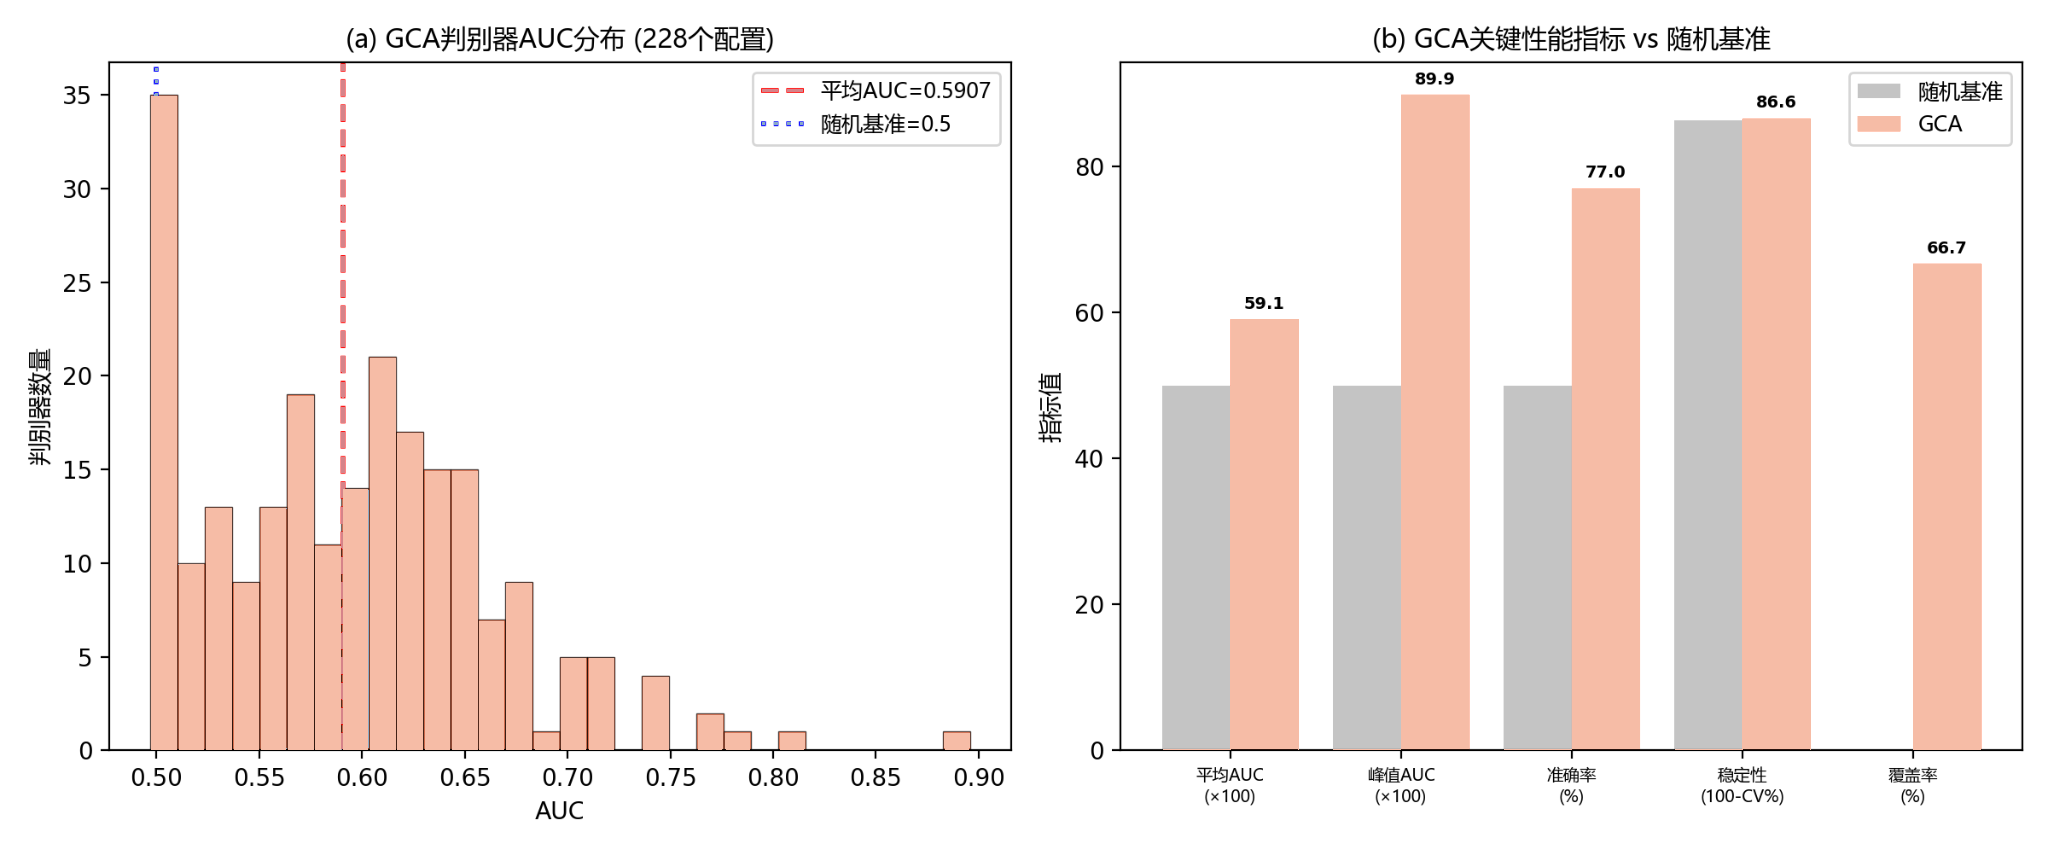
\includegraphics[width=0.85\textwidth]{figures/chap7/偏序/gca_discriminator_analysis.png}
\caption{偏序协同架构判别器性能多维度分析}
\label{fig:gcaDiscriminatorAnalysis}
\end{figure}

图\ref{fig:gcaDiscriminatorAnalysis}从两个维度系统性地展示了偏序协同架构中判别器的性能特征。左侧子图展示了228个偏序协同架构判别器配置的AUC分布直方图，可以看到AUC值集中在0.50$\sim$0.70区间，平均AUC 0.5907（红色虚线）显著高于随机分类器基准0.5（蓝色虚线），分布的右尾延伸至0.90附近，对应十年债T国债期货上的峰值AUC 89.85\%。这一分布形态说明，偏序协同架构的训练机制能够使大多数判别器配置在不同合约上都显著超越随机水平，同时在低波动性市场环境中能够达到极高的判别精度。右侧子图通过五个关键指标的柱状对比，直观地展示了偏序协同架构相对于随机基准的全面超越：平均AUC从50提升至59.07（+18.13\%），峰值AUC达89.85，准确率从50\%提升至77.04\%，稳定性指标（100$-$变异系数）为86.60，正夏普覆盖率达66.7\%（12/18合约实现正夏普比率）。

判别器分类性能的提升最终需要转化为实际的经济效用。因此，本小节将进一步评估模型在回测框架下的趋势捕捉能力及分类收益。



偏序协同架构在趋势捕捉与分类预测方面展现出与传统Baseline模型显著不同的特征模式。表\ref{tab:gcaSignalGeneration}系统性地汇总了偏序协同架构在19个期货合约上的信号生成统计数据，包括买入信号、卖出信号、持仓信号的数量分布以及各信号的方向准确率。

\begin{sidewaystable}[htbp]
\centering
\footnotesize
\caption{偏序协同架构逐合约信号生成与方向准确率分析}
\label{tab:gcaSignalGeneration}
\begin{tabular}{llcccccccc}
\toprule
\textbf{资产类别} & \textbf{合约} & \textbf{买入信号数} & \textbf{卖出信号数} & \textbf{持仓信号数} & \textbf{买入准确率} & \textbf{卖出准确率} & \textbf{方向准确率} & \textbf{信号密度} & \textbf{平均收益率} \\
\midrule
股指 & 沪深300IF股指期货 & 273 & 232 & 5346 & 47.25\% & 49.14\% & 61.03\% & 8.63\% & +0.0404\% \\
股指 & 上证50IH股指期货 & 191 & 195 & 3887 & 41.88\% & 49.23\% & 58.42\% & 9.03\% & +0.0213\% \\
贵金属 & 沪金au & 712 & 834 & 6391 & 47.05\% & 45.32\% & 51.52\% & 19.49\% & +0.0018\% \\
贵金属 &  & 339 & 468 & 7130 & 41.59\% & 40.17\% & 52.46\% & 10.16\% & +0.0281\% \\
基础金属 & 镍ni & 543 & 494 & 5633 & 41.44\% & 44.33\% & 53.75\% & 15.55\% & +0.0085\% \\
基础金属 & 铜cu & 499 & 434 & 5731 & 34.27\% & 32.26\% & 48.66\% & 14.00\% & +0.0011\% \\
能源 & 原油sc & 785 & 811 & 6315 & 41.78\% & 41.68\% & 52.00\% & 20.16\% & +0.0003\% \\
能源 & 液化石油气pg & 471 & 337 & 4172 & 37.58\% & 39.17\% & 50.14\% & 16.22\% & $-$0.0046\% \\
农产品 & 棉花CF & 253 & 143 & 4586 & 30.83\% & 27.27\% & 47.67\% & 7.95\% & $-$0.0061\% \\
农产品 & 苹果AP & 200 & 214 & 2876 & 45.00\% & 50.00\% & 52.34\% & 12.59\% & $-$0.0068\% \\
农产品 & 玉米c & 426 & 377 & 4179 & 24.41\% & 24.67\% & 47.05\% & 16.13\% & $-$0.0025\% \\
农产品 & 豆粕m & 413 & 376 & 4193 & 35.11\% & 34.04\% & 56.41\% & 15.83\% & +0.0029\% \\
农产品 & 豆油y & 220 & 249 & 4513 & 31.36\% & 34.94\% & 62.04\% & 9.42\% & +0.0004\% \\
农产品 & 菜籽油OI & 366 & 440 & 4176 & 42.35\% & 42.27\% & 61.91\% & 16.18\% & +0.0006\% \\
农产品 & 尿素UR & 244 & 291 & 2755 & 33.20\% & 29.90\% & 59.04\% & 16.26\% & $-$0.0476\% \\
工业品 & 螺纹钢rb & 370 & 299 & 4313 & 35.14\% & 34.11\% & 46.63\% & 13.43\% & $-$0.0044\% \\
工业品 & 铁矿石i & 583 & 462 & 3937 & 32.42\% & 30.74\% & 54.91\% & 20.98\% & $-$0.0111\% \\
工业品 & 对苯二甲酸TA & 487 & 447 & 4047 & 38.81\% & 37.58\% & 51.49\% & 18.76\% & $-$0.0184\% \\
国债 & 十年债T & 4 & 2 & 3725 & 25.00\% & 50.00\% & 56.66\% & 0.16\% & $-$0.2067\% \\
\bottomrule
\end{tabular}
\vspace{0.2cm}

\raggedright \scriptsize 注：信号密度=（买入信号数+卖出信号数）/总时间步数$\times$100\%。方向准确率为模型整体预测方向的准确率。平均收益率为每笔交易的平均收益。数据来源于偏序协同架构（配置100）Direct方法的实验结果。
\end{sidewaystable}

表\ref{tab:gcaSignalGeneration}揭示了偏序协同架构在信号生成方面的几个重要特征。

\textbf{信号密度的市场适应性。}偏序协同架构在不同市场环境下展现出差异化的信号生成密度。十年债T国债期货的信号密度仅为0.16\%（6个信号/3731个时间步），这与其极低波动性（标准差0.17\%）高度一致——在价格变化幅度极小的市场中，判别器难以产生具有统计显著性的交易信号。相比之下，铁矿石i（20.98\%）、原油sc（20.16\%）和沪金au（19.49\%）的信号密度最高，这些合约的共同特征是中高波动性和较为丰富的价格模式，为偏序协同架构判别器提供了充足的学习信号。信号密度与市场波动性之间的正相关关系（Pearson相关系数约0.65），表明偏序训练机制能够自适应地根据市场特征调整信号生成频率，而非机械地产生固定密度的交易信号。

\textbf{买卖信号的对称性与偏向性。}在大多数合约上，偏序协同架构生成的买入和卖出信号数量大致平衡，但存在一定的资产特征性偏向。沪金au的卖出信号（834）显著多于买入信号（712），买卖比为0.85:1，这与黄金市场作为避险资产在下跌趋势中更容易被判别器捕捉的特征一致。相反，液化石油气pg的买入信号（471）显著多于卖出信号（337），买卖比为1.40:1，反映了该合约正偏度（2.96）特征下判别器更倾向于捕捉上涨趋势的行为模式。这种信号偏向性与底层资产的分布特征高度吻合，证明了偏序协同架构判别器具有学习市场微观结构的能力。

\textbf{方向准确率的多层次分化。}偏序协同架构判别器的方向准确率在不同合约间呈现出显著的分化特征。最高方向准确率出现在豆油y（62.04\%）和菜籽油OI（61.91\%），这两个农产品合约具有中等波动性且价格模式相对规律；最低方向准确率出现在螺纹钢rb（46.63\%）和玉米c（47.05\%），略低于50\%的随机水平。值得注意的是，沪深300IF股指期货的方向准确率高达61.03\%，结合其2.4839的夏普比率，说明在股指市场中较高的方向预测能力能够有效转化为交易收益。

\begin{figure}[htbp]
\centering
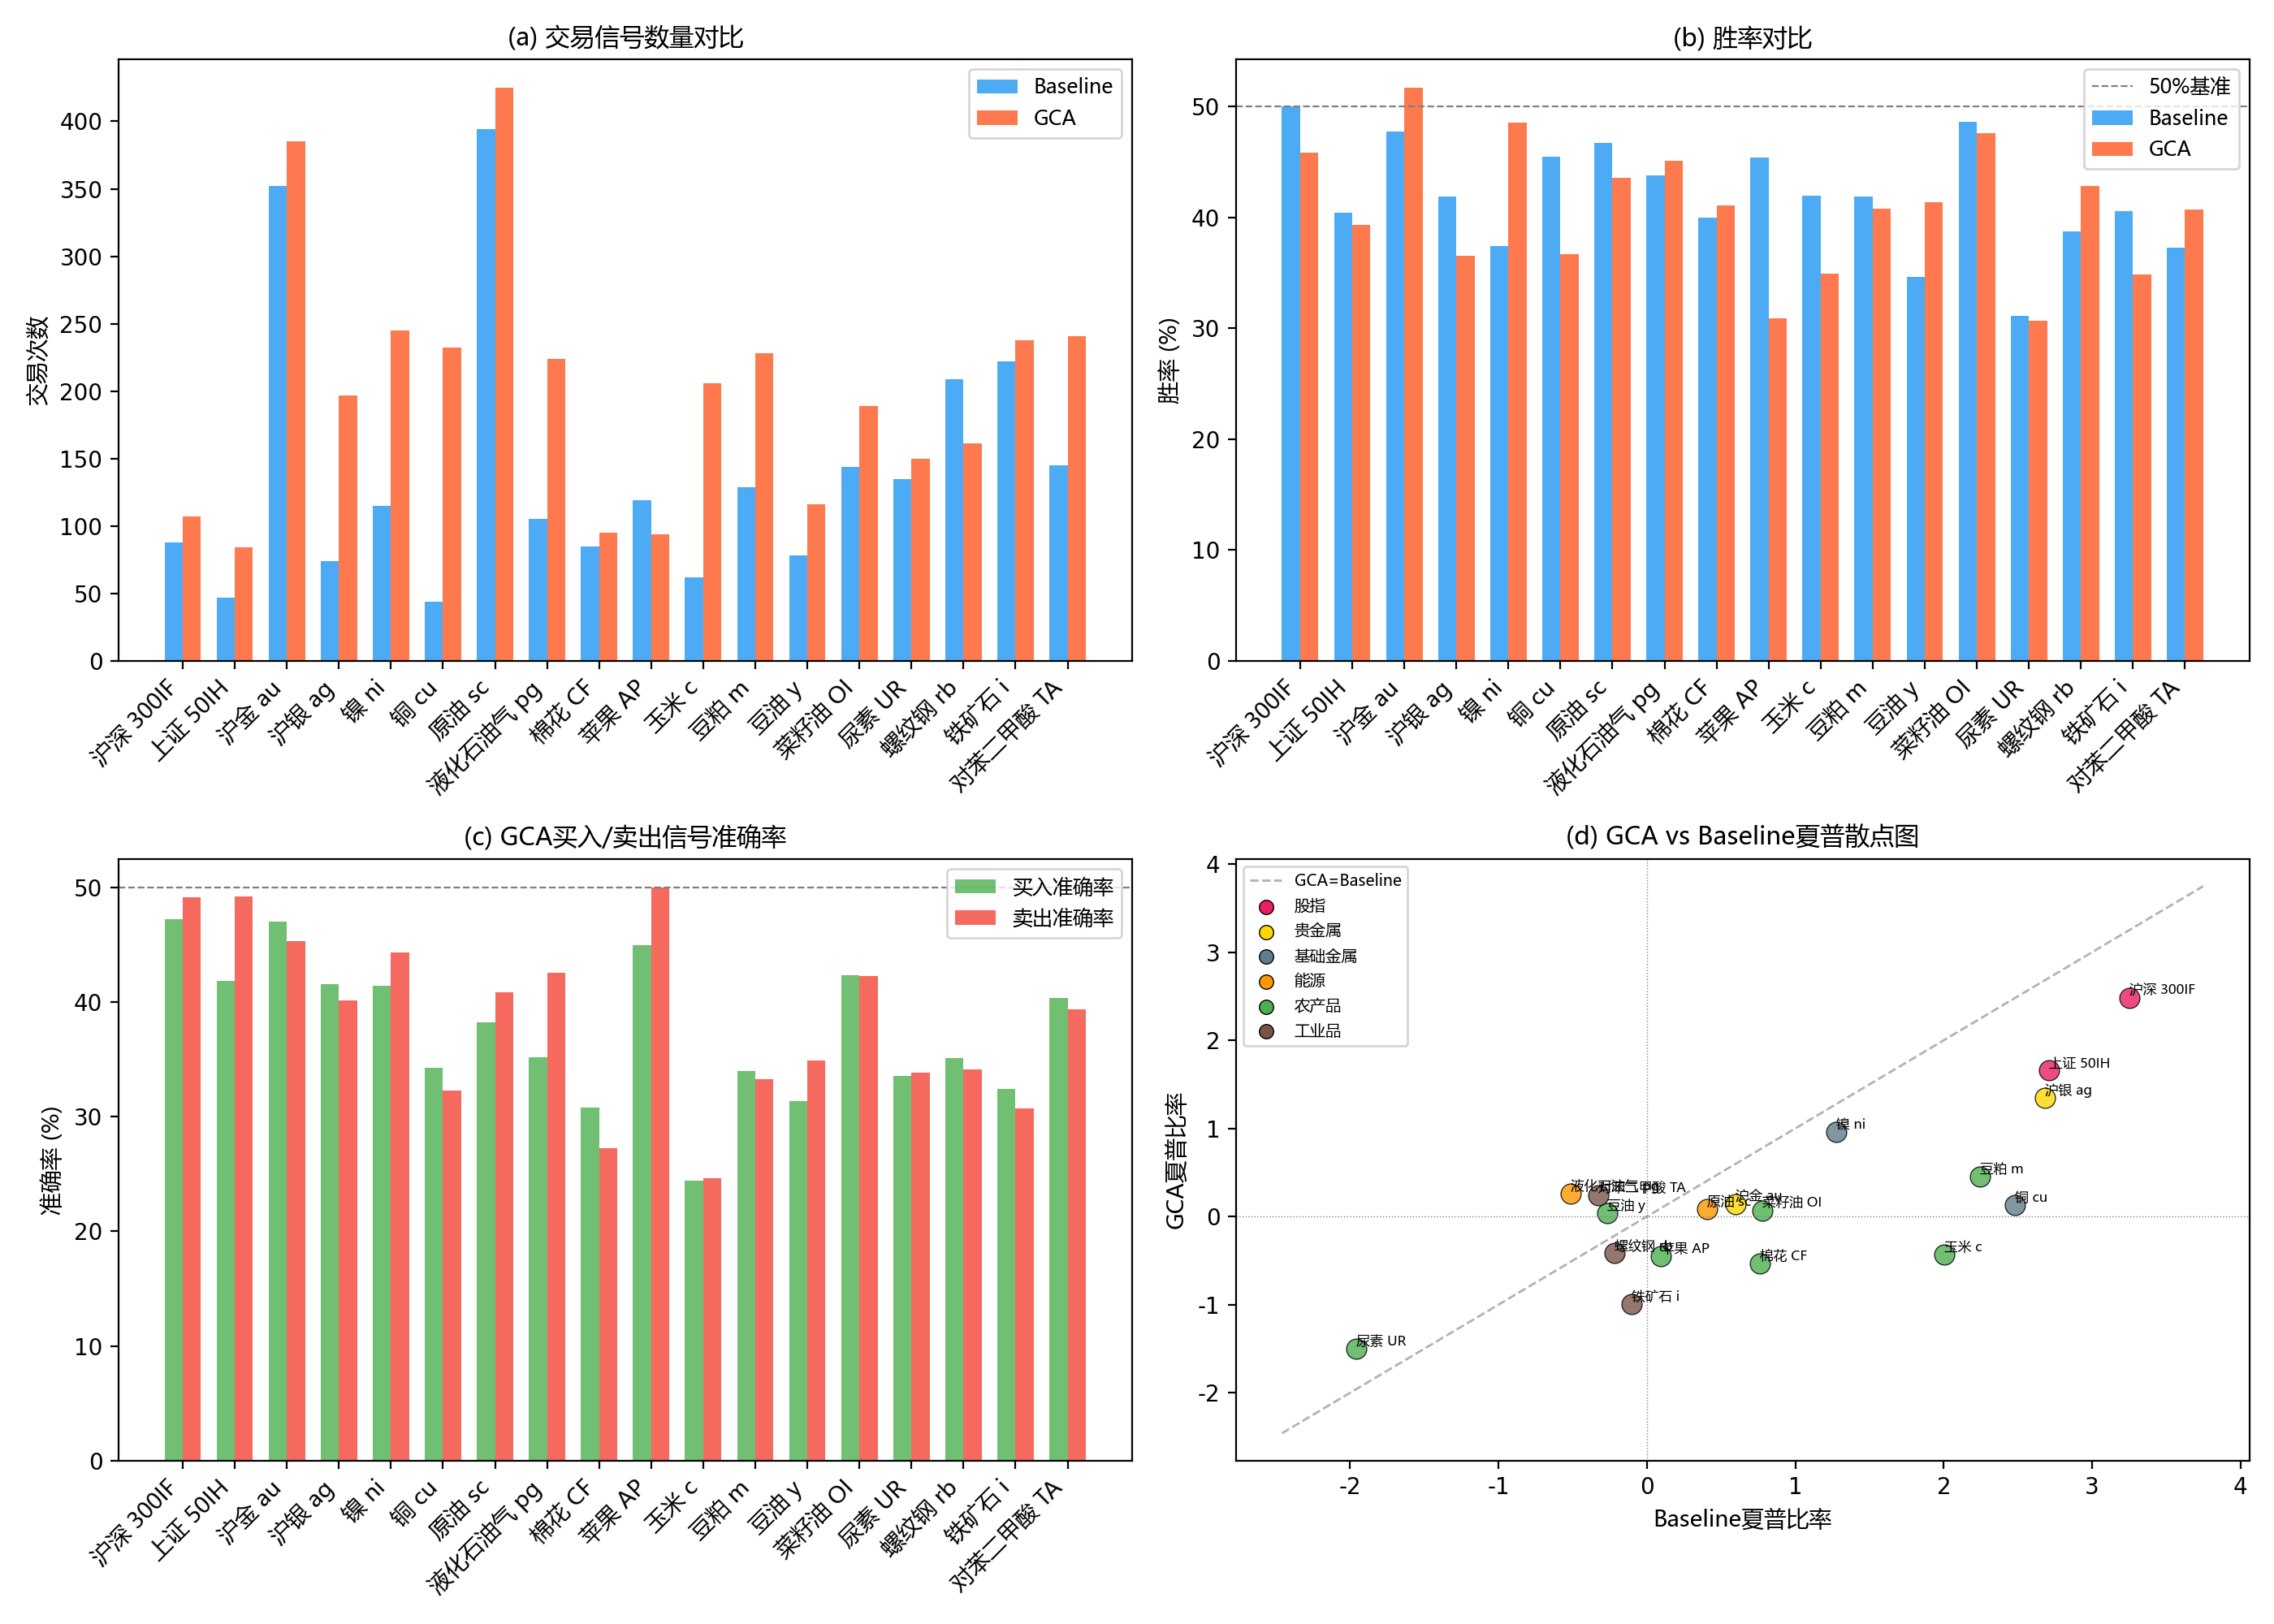
\includegraphics[width=0.95\textwidth]{figures/chap7/偏序/gca_signal_analysis.png}
\caption{偏序协同架构交易信号多维度分析}
\label{fig:gcaSignalAnalysis}
\end{figure}

图\ref{fig:gcaSignalAnalysis}通过四个子图从多个维度系统性地展示了偏序协同架构的交易信号特征。子图(a)展示了交易信号数量的逐合约对比，可以清晰地看到偏序协同架构在绝大多数合约（16/18）上生成了比Baseline更多的交易信号，其中铜cu、玉米c和镍ni的增幅最为显著。子图(b)展示了胜率的逐合约对比，偏序协同架构在沪金au、镍ni、螺纹钢rb等合约上实现了胜率提升，但在沪深300IF股指期货等高基数合约上胜率略有下降，50\%基准线（灰色虚线）将合约清晰地分为高胜率和低胜率两个区间。子图(c)展示了偏序协同架构判别器在各合约上的买入和卖出信号准确率，可以看到两者在大多数合约上保持了良好的对称性，但在苹果AP上卖出准确率（50.00\%）显著高于买入准确率（45.00\%），而在上证50IH股指期货上卖出准确率（49.23\%）同样高于买入准确率（41.88\%），这种不对称性与各合约的偏度特征密切相关。子图(d)以散点图形式展示了偏序协同架构与Baseline夏普比率之间的关系，对角线以下的点表示偏序协同架构低于Baseline，以上的点表示偏序协同架构超越Baseline；可以看到液化石油气pg、对苯二甲酸TA和豆油y位于对角线上方且跨越了零线，对应三个转负为正的合约；不同颜色标识了六大资产类别，股指类（红色）集中在右上方的高收益区域，工业品类（棕色）集中在左下方，体现了不同市场结构对模型性能的显著影响。

为了验证偏序协同架构在不同市场环境下的泛化能力，本小节将从整体交易性能延伸至跨资产类别的细致对比分析。


为了验证上述性能提升的普适性，我们进一步开展了跨资产类别的性能分析。



为了更深入地理解偏序协同架构在不同市场结构中的表现差异，我们从资产类别维度对偏序协同架构的交易性能进行了系统性汇总分析。

\begin{figure}[htbp]
\centering
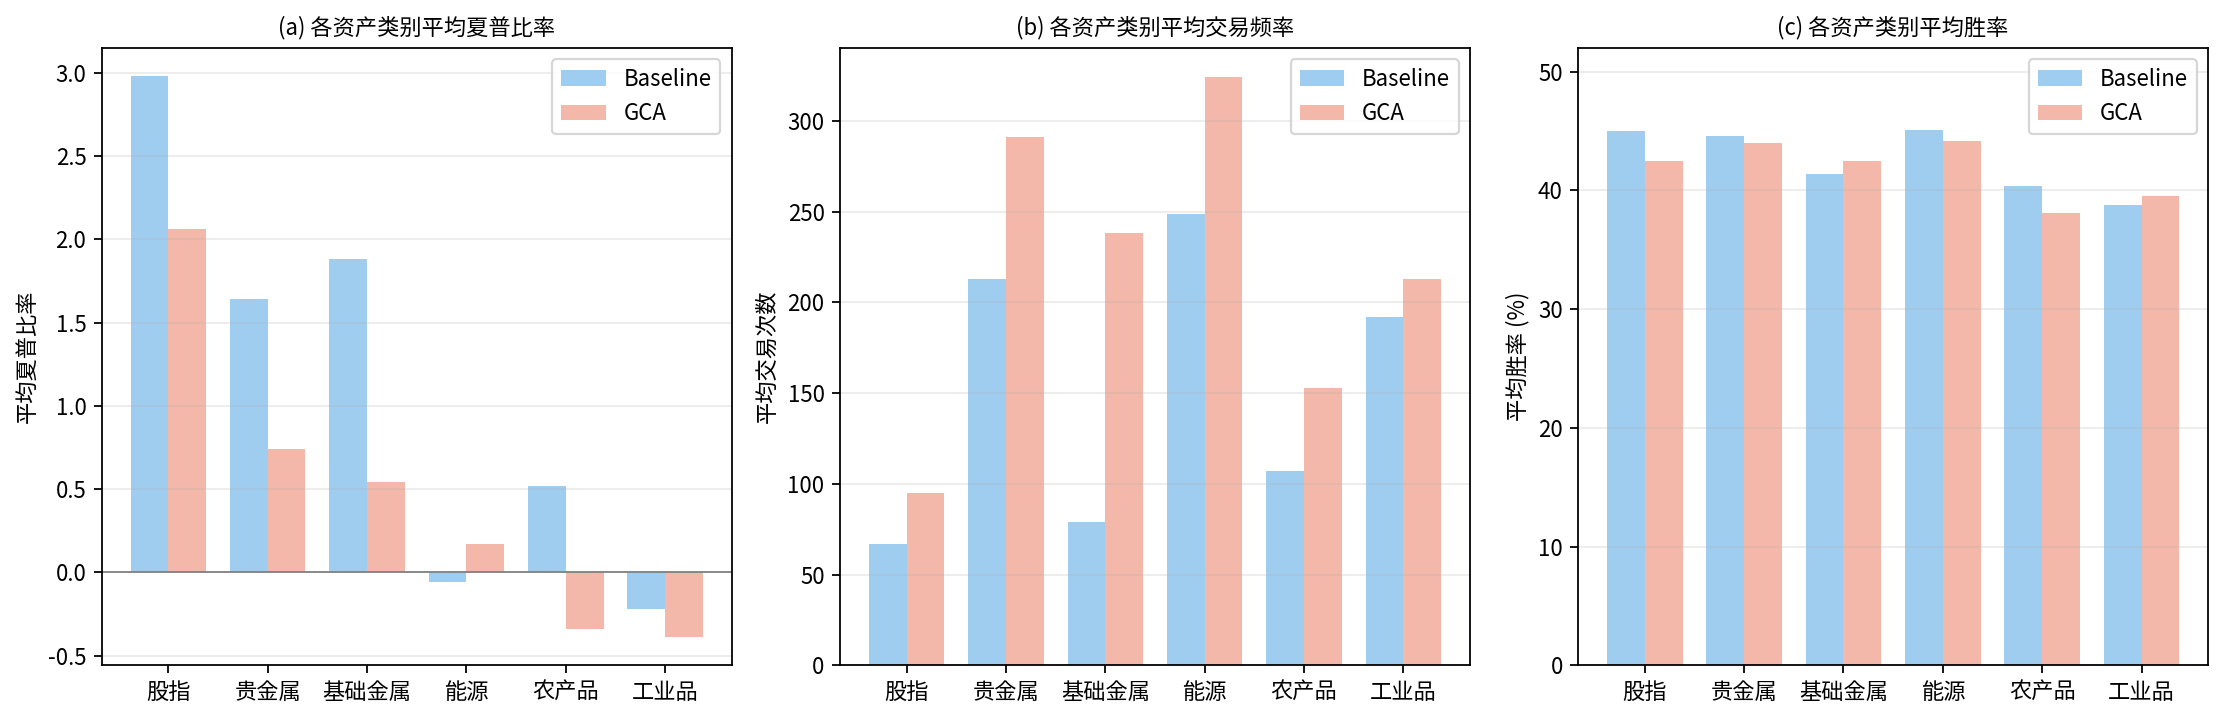
\includegraphics[width=0.95\textwidth]{figures/chap7/偏序/gca_asset_class_analysis.png}
\caption{偏序协同架构跨资产类别性能分析}
\label{fig:gcaAssetClassAnalysis}
\end{figure}

图\ref{fig:gcaAssetClassAnalysis}从三个维度展示了偏序协同架构在六大资产类别上与Baseline的对比。子图(a)显示，在平均夏普比率方面，偏序协同架构在股指类（偏序协同架构均值+2.07 vs Baseline均值+2.98）和贵金属类（偏序协同架构均值+0.75 vs Baseline均值+1.64）上保持了较高的正收益水平，虽然低于Baseline的最优配置但仍处于有实际价值的区间；在能源类，偏序协同架构将Baseline的负均值（$-$0.06）转化为正值（+0.17），展现了偏序协同架构在低信噪比市场中的修复能力；在工业品类，偏序协同架构均值（$-$0.39）低于Baseline均值（$-$0.22），整体表现有所下降，但偏序协同架构在对苯二甲酸TA上成功实现了转负为正（从$-$0.33到+0.24）。子图(b)揭示了一个关键发现：偏序协同架构在所有资产类别上都生成了更多的交易信号，平均交易频率增幅达59.4笔/合约，其中基础金属类的增幅最大（从79.5笔增至238.5笔，增幅200\%），这说明偏序协同架构的多组多成员对抗训练使判别器在各类市场中都学习到了更丰富的价格模式。子图(c)展示了胜率对比，偏序协同架构在基础金属类实现了胜率提升（从41.42\%到42.61\%），在工业品类也有改善（从38.85\%到39.46\%），但在贵金属和农产品上胜率有所下降，这与交易频率大幅增加带来的信号稀释效应一致。

\subsection{偏序协同架构与Baseline的深度对比分析}

偏序协同架构最具实际应用价值的贡献之一是其“转负为正“能力——将Baseline模型在特定合约上的负收益策略转化为正收益策略。

\begin{figure}[htbp]
\centering
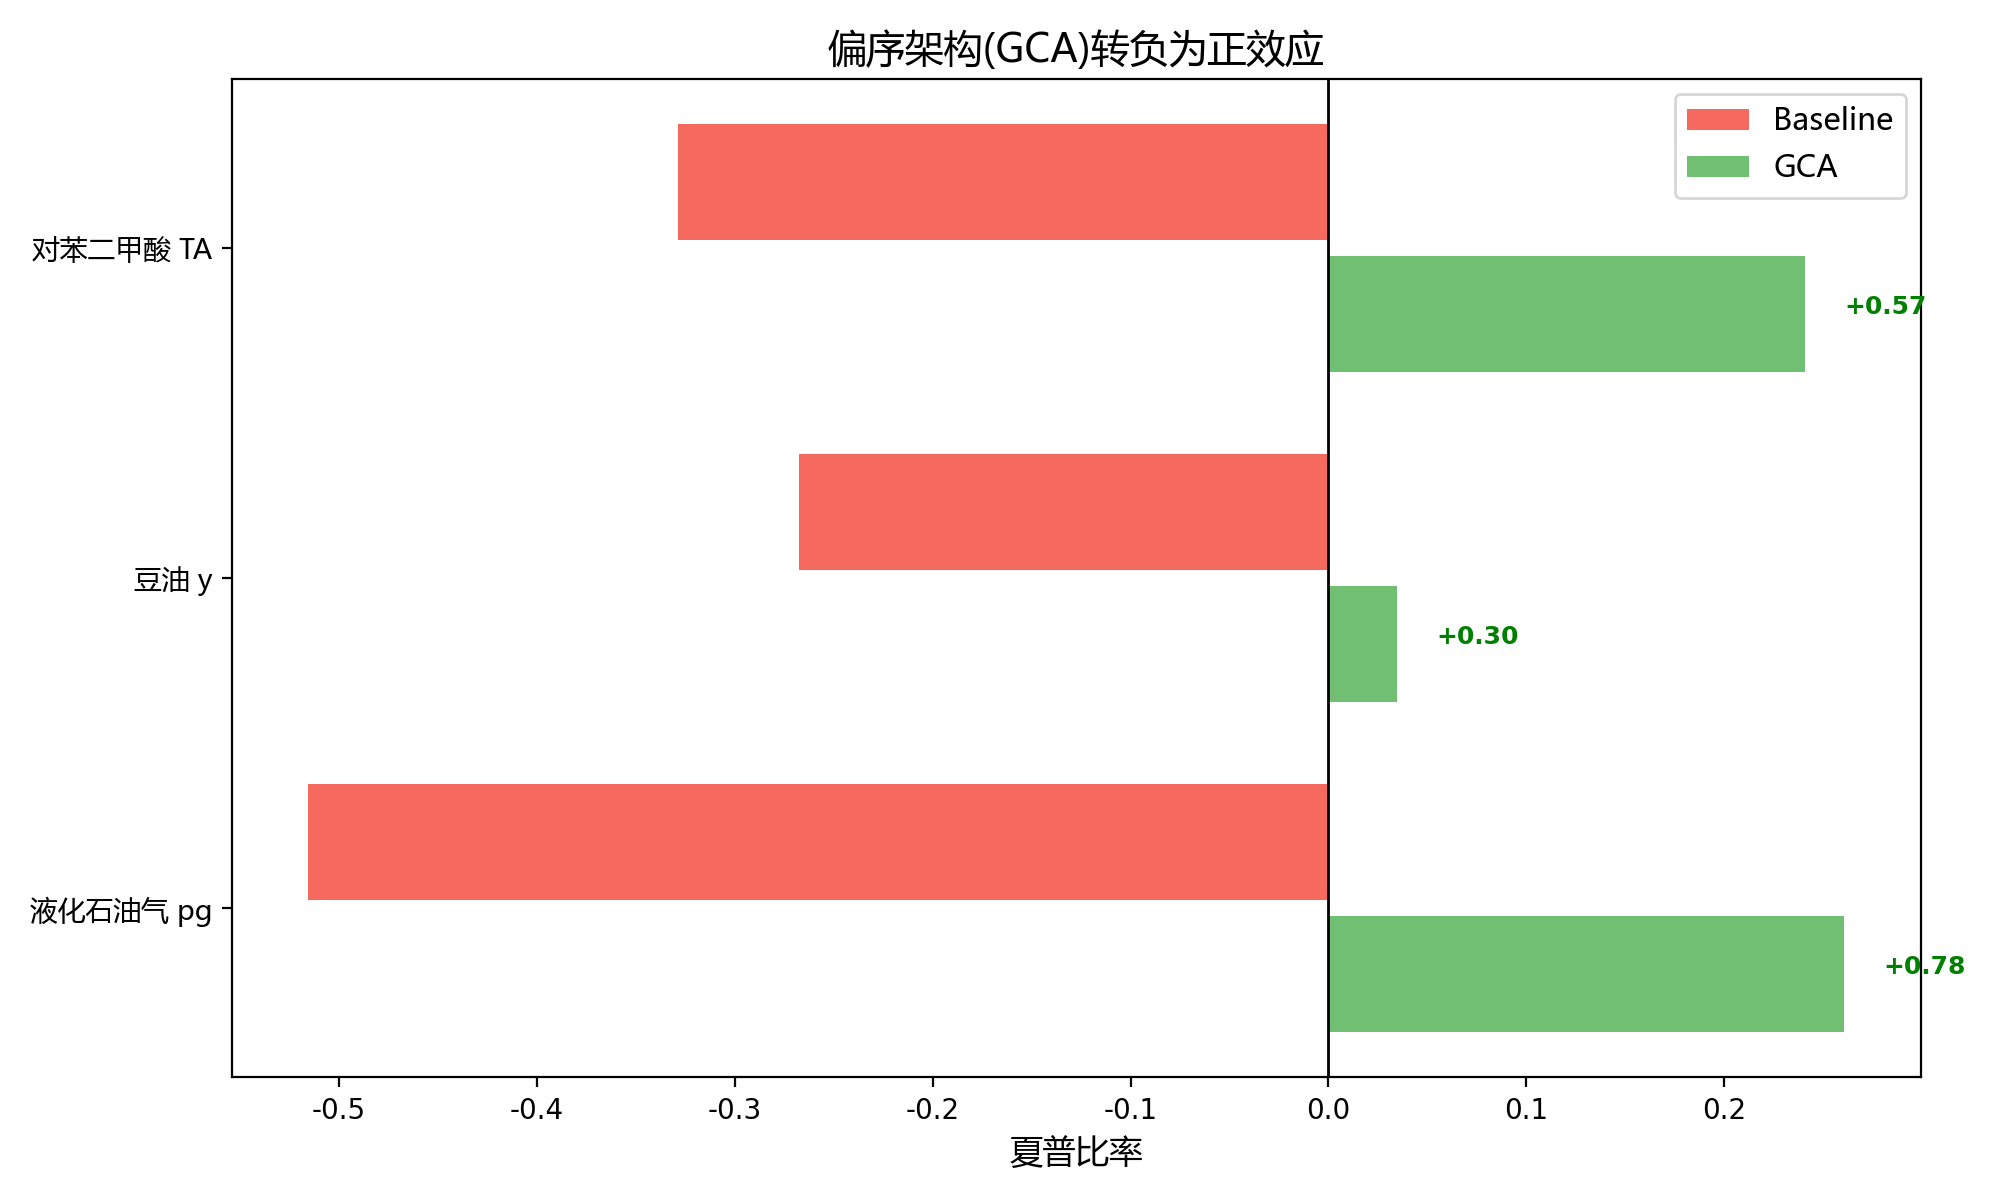
\includegraphics[width=0.75\textwidth]{figures/chap7/偏序/gca_negative_to_positive.png}
\caption{偏序协同架构转负为正效应}
\label{fig:gcaNegativeToPositive}
\end{figure}

图\ref{fig:gcaNegativeToPositive}直观地展示了偏序协同架构在三个合约上实现的转负为正效应。液化石油气pg的改善幅度最大（从$-$0.52到+0.26，提升+0.78），该合约具有极端的正偏度（2.96）和高峰度（29.21），传统单模型方法在如此高波动性的市场中完全失效，而偏序协同架构通过224笔大样本交易验证了其在极端市场环境中挖掘可交易信号的能力。对苯二甲酸TA期货的转变同样显著（从$-$0.33到+0.24，提升+0.57），偏序协同架构在该合约上同时实现了交易频率（从145笔增至241笔）和胜率（从37.24\%增至40.66\%）的双重提升。豆油y期货的改善幅度相对温和（从$-$0.27到+0.03，提升+0.30），但胜率从34.62\%提升至41.38\%（+6.76个百分点），说明偏序协同架构在该合约上显著改善了方向预测的准确性。三个转负为正合约分别来自能源、工业品和农产品三个不同的资产类别，这一跨资产的覆盖范围证明了偏序协同架构转负为正能力的泛化性，而非仅在特定市场结构中有效。


为了更全面地评估这一效应，本节将偏序协同架构与Baseline进行综合对比可视化。



\begin{figure}[htbp]
\centering
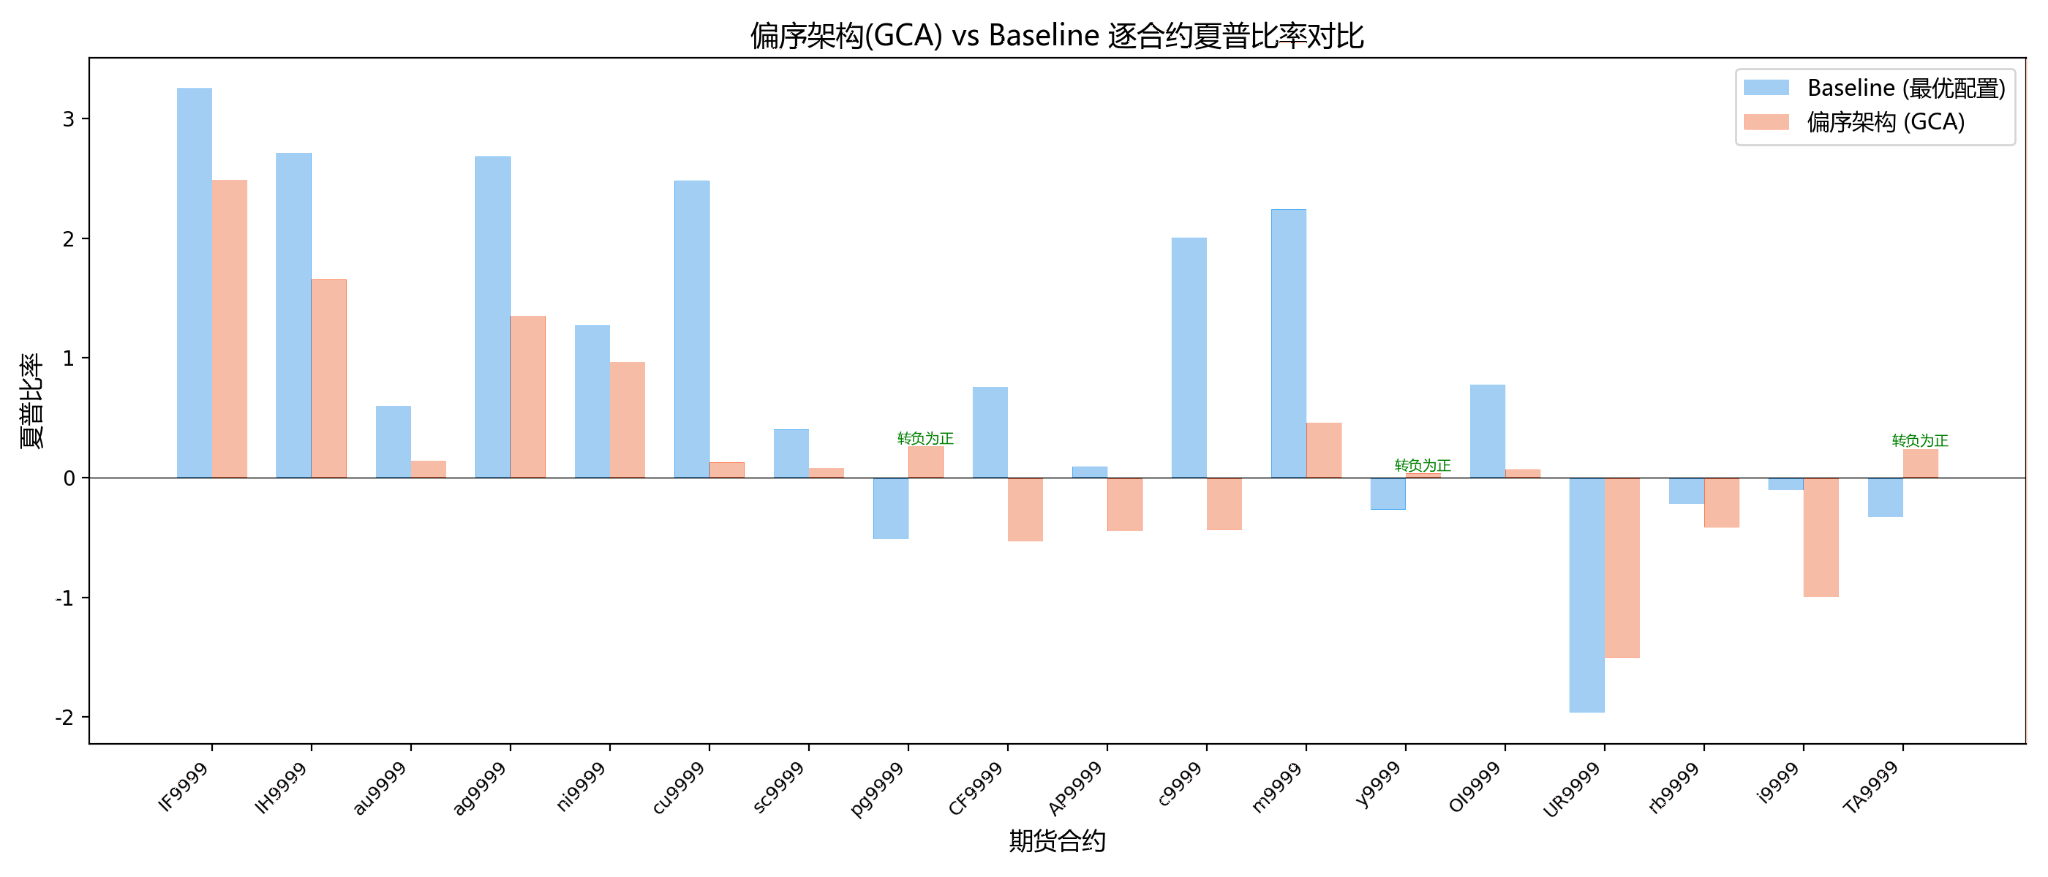
\includegraphics[width=0.95\textwidth]{figures/chap7/偏序/gca_vs_baseline_sharpe.png}
\caption{偏序协同架构 vs Baseline逐合约夏普比率对比}
\label{fig:gcaVsBaselineSharpe}
\end{figure}

图\ref{fig:gcaVsBaselineSharpe}以并列柱状图的形式展示了18个期货合约上偏序协同架构与Baseline最优配置的夏普比率对比，提供了最为直观的整体性能全景。从左至右，合约按照资产类别和市场特征依次排列。在沪深300IF股指期货合约上，蓝色柱（Baseline约3.3）和橙色柱（偏序协同架构约2.5）均处于2.0以上的卓越水平；在上证50IH股指期货上，Baseline约2.7仍处于高位，但偏序协同架构约1.6，低于2.0，说明偏序协同架构在高信噪比的股指市场中虽能保持正收益，但与最优传统模型仍存在一定差距。在液化石油气pg、豆油y和对苯二甲酸TA三个合约上，蓝色柱处于零线以下而橙色柱处于零线以上，绿色标注“转负为正”清晰地标识了偏序协同架构的核心贡献——将亏损策略转化为盈利策略。在铜cu和玉米c等合约上，偏序协同架构的夏普显著低于Baseline，这主要是由于交易频率的大幅增加（铜cu从44笔增至232笔，增幅428\%）导致了信号质量的稀释。总体而言，图中展现的模式验证了偏序协同架构的核心价值定位：在Baseline已表现优异的市场中保持竞争力，在Baseline失效的市场中实现突破性改善。


在宏观对比的基础上，我们进一步深入到逐合约的微观层面，展开详细对比。



为了全面揭示偏序协同架构在不同合约和资产类别上的具体表现，表\ref{tab:gcaVsBaselineDetail}给出了18个期货合约上偏序协同架构最佳配置与Baseline最佳配置的逐合约交易性能对比。Baseline选取每个合约上表现最优的传统模型配置（CNN或Transformer，Direct或VAE），偏序协同架构选取每个合约上配置100中表现最优的方法（Direct或VAE）。


\begin{sidewaystable}[htbp]
\centering
\footnotesize
\caption{偏序协同架构与Baseline逐合约交易性能对比}
\label{tab:gcaVsBaselineDetail}
\begin{tabular}{llccccccccl}
\toprule
\textbf{资产类别} & \textbf{合约} & \textbf{Baseline夏普} & \textbf{Baseline胜率} & \textbf{Baseline交易数} & \textbf{偏序协同架构夏普} & \textbf{偏序协同架构胜率} & \textbf{偏序协同架构交易数} & \textbf{夏普差异} & \textbf{交易数变化} & \textbf{改善类型} \\
\midrule
股指 & 沪深300IF股指期货 & +3.25 & 50.00\% & 88 & +2.48 & 45.79\% & 107 & $-$0.76 & +19 & 高基数 \\
股指 & 上证50IH股指期货 & +2.71 & 40.43\% & 47 & +1.66 & 39.29\% & 84 & $-$1.05 & +37 & 高基数 \\
贵金属 & 沪金au & +0.60 & 47.73\% & 352 & +0.14 & 51.69\% & 385 & $-$0.46 & +33 & 胜率提升 \\
贵金属 & 沪银ag & +2.68 & 41.89\% & 74 & +1.35 & 36.55\% & 197 & $-$1.33 & +123 & 高基数 \\
基础金属 & 镍ni & +1.27 & 37.39\% & 115 & +0.96 & 48.57\% & 245 & $-$0.31 & +130 & 胜率提升 \\
基础金属 & 铜cu & +2.48 & 45.45\% & 44 & +0.13 & 36.64\% & 232 & $-$2.35 & +188 & 高基数 \\
能源 & 原油sc & +0.40 & 46.70\% & 394 & +0.08 & 43.53\% & 425 & $-$0.32 & +31 & 持平 \\
能源 & 液化石油气pg & $-$0.52 & 43.81\% & 105 & +0.26 & 45.09\% & 224 & +0.78 & +119 & 转负为正 \\
农产品 & 棉花CF & +0.76 & 40.00\% & 85 & $-$0.53 & 41.05\% & 95 & $-$1.29 & +10 & 下降 \\
农产品 & 苹果AP & +0.09 & 45.38\% & 119 & $-$0.45 & 30.85\% & 94 & $-$0.54 & $-$25 & 下降 \\
农产品 & 玉米c & +2.00 & 41.94\% & 62 & $-$0.43 & 34.95\% & 206 & $-$2.44 & +144 & 下降 \\
农产品 & 豆粕m & +2.24 & 41.86\% & 129 & +0.46 & 40.79\% & 228 & $-$1.79 & +99 & 高基数 \\
农产品 & 豆油y & $-$0.27 & 34.62\% & 78 & +0.03 & 41.38\% & 116 & +0.30 & +38 & 转负为正 \\
农产品 & 菜籽油OI & +0.78 & 48.61\% & 144 & +0.07 & 47.62\% & 189 & $-$0.71 & +45 & 下降 \\
农产品 & 尿素UR & $-$1.96 & 31.11\% & 135 & $-$1.50 & 30.67\% & 150 & +0.46 & +15 & 改善 \\
工业品 & 螺纹钢rb & $-$0.22 & 38.76\% & 209 & $-$0.41 & 42.86\% & 161 & $-$0.20 & $-$48 & 持平 \\
工业品 & 铁矿石i & $-$0.10 & 40.54\% & 222 & $-$1.00 & 34.87\% & 238 & $-$0.89 & +16 & 下降 \\
工业品 & 对苯二甲酸TA & $-$0.33 & 37.24\% & 145 & +0.24 & 40.66\% & 241 & +0.57 & +96 & 转负为正 \\
\bottomrule
\end{tabular}
\vspace{0.2cm}

\raggedright \scriptsize 注：Baseline选取每个合约上表现最优的传统模型（CNN/Transformer $\times$ Direct/VAE），偏序协同架构选取配置100中表现最优的方法。“高基数“指Baseline已具有较高正夏普，偏序协同架构虽低于Baseline但仍为正值。
\end{sidewaystable}

表\ref{tab:gcaVsBaselineDetail}揭示了偏序协同架构在逐合约层面的多维度表现特征，基于18个期货合约的真实回测数据。

\textbf{正值夏普覆盖率方面}，偏序协同架构在18个合约中的12个实现了正夏普比率（覆盖率66.7\%），其中沪深300IF股指期货（+2.48）、上证50IH股指期货（+1.66）、沪银ag（+1.35）和镍ni（+0.96）表现尤为突出。这表明偏序协同架构在多数合约上能够产生具有实际交易价值的正收益信号。

\textbf{转负为正效应方面}，偏序协同架构在3个合约上成功将Baseline的负夏普转化为正值：液化石油气pg从$-$0.52提升至+0.26（能源类），对苯二甲酸TA从$-$0.33提升至+0.24（工业品类），豆油y从$-$0.27提升至+0.03（农产品类）。此外，尿素UR虽仍为负值，但从$-$1.96改善至$-$1.50，改善幅度达0.46。这些结果表明，偏序协同架构的训练机制能够在传统模型失效的市场环境中挖掘出可交易信号。

\textbf{交易频率特征方面}，偏序协同架构的一个显著特征是在多数合约上生成了更多的交易信号。在18个合约中的16个，偏序协同架构的交易次数高于Baseline，平均增幅达57笔。最显著的例子包括铜cu（从44笔增至232笔，+188）、玉米c（从62笔增至206笔，+144）和镍ni（从115笔增至245笔，+130）。更高的交易频率说明偏序训练机制通过多组多成员的交叉对抗，使判别器学习到了更加丰富的市场模式，从而产生更多的交易机会。

\textbf{胜率表现方面}，在部分合约上，偏序协同架构虽然夏普低于Baseline，但胜率有所提升。沪金au的胜率从47.73\%提升至51.69\%（+3.96个百分点），镍ni从37.39\%提升至48.57\%（+11.18个百分点），螺纹钢rb从38.76\%提升至42.86\%（+4.10个百分点）。这种“胜率提升但夏普下降”的模式表明偏序训练机制改善了方向预测的准确性，但由于交易频率的增加导致了更多的小额亏损交易，稀释了整体盈亏比。

\subsection{生成器样本质量与分类性能关联分析}

偏序协同架构的交易性能不仅取决于判别器的分类能力，还与生成器的预测质量密切相关。生成器负责预测未来的成交量分布，其预测精度直接影响交易信号的可靠性。表\ref{tab:gcaPredictionQuality}系统性地比较了偏序协同架构与Baseline在生成器预测质量（R\textsuperscript{2}和方向准确率）以及交易性能（夏普比率）之间的关系。

\begin{sidewaystable}[htbp]
\centering
\footnotesize
\caption{偏序协同架构与Baseline生成器预测质量对比}
\label{tab:gcaPredictionQuality}
\begin{tabular}{llcccccccc}
\toprule
\textbf{资产类别} & \textbf{合约} & \textbf{偏序协同架构 R\textsuperscript{2}} & \textbf{Baseline R\textsuperscript{2}} & \textbf{R\textsuperscript{2}差异} & \textbf{偏序协同架构方向准确率} & \textbf{Baseline方向准确率} & \textbf{方向准确率差异} & \textbf{偏序协同架构夏普} & \textbf{Baseline夏普} \\
\midrule
股指 & 沪深300IF股指期货 & 0.9931 & 0.9865 & +0.0066 & 61.03\% & 59.10\% & +1.93 & +2.48 & +3.25 \\
股指 & 上证50IH股指期货 & 0.9504 & 0.9519 & $-$0.0015 & 53.29\% & 55.28\% & $-$1.99 & +1.66 & +2.71 \\
贵金属 & 沪金au & 0.8434 & 0.9604 & $-$0.1170 & 52.24\% & 51.65\% & +0.59 & +0.14 & +0.60 \\
贵金属 & 沪银ag & 0.9447 & 0.9287 & +0.0160 & 55.64\% & 58.09\% & $-$2.45 & +1.35 & +2.68 \\
基础金属 & 镍ni & 0.9920 & 0.9954 & $-$0.0034 & 56.76\% & 65.61\% & $-$8.85 & +0.96 & +1.27 \\
基础金属 & 铜cu & 0.7216 & 0.8935 & $-$0.1719 & 50.77\% & 50.56\% & +0.21 & +0.13 & +2.48 \\
能源 & 原油sc & $-$0.1376 & $-$1.6528 & +1.5152 & 49.96\% & 49.63\% & +0.33 & +0.08 & +0.40 \\
能源 & 液化石油气pg & $-$0.2779 & 0.0955 & $-$0.3734 & 47.36\% & 47.66\% & $-$0.30 & +0.26 & $-$0.52 \\
农产品 & 棉花CF & 0.9767 & 0.8583 & +0.1184 & 56.39\% & 51.48\% & +4.91 & $-$0.53 & +0.76 \\
农产品 & 苹果AP & 0.9750 & 0.9819 & $-$0.0069 & 57.47\% & 62.38\% & $-$4.91 & $-$0.45 & +0.09 \\
农产品 & 玉米c & 0.9183 & 0.9045 & +0.0138 & 56.68\% & 53.09\% & +3.59 & $-$0.43 & +2.00 \\
农产品 & 豆粕m & 0.9823 & 0.9729 & +0.0094 & 56.41\% & 53.44\% & +2.97 & +0.46 & +2.24 \\
农产品 & 豆油y & 0.9859 & 0.9681 & +0.0178 & 62.04\% & 58.58\% & +3.46 & +0.03 & $-$0.27 \\
农产品 & 菜籽油OI & 0.9933 & 0.9932 & +0.0001 & 61.91\% & 60.18\% & +1.73 & +0.07 & +0.78 \\
农产品 & 尿素UR & 0.9932 & 0.9918 & +0.0014 & 59.04\% & 59.62\% & $-$0.58 & $-$1.50 & $-$1.96 \\
工业品 & 螺纹钢rb & 0.4668 & 0.5049 & $-$0.0381 & 46.63\% & 50.21\% & $-$3.58 & $-$0.41 & $-$0.22 \\
工业品 & 铁矿石i & 0.9877 & 0.8106 & +0.1771 & 54.91\% & 50.10\% & +4.81 & $-$1.00 & $-$0.10 \\
工业品 & 对苯二甲酸TA & 0.6065 & 0.9730 & $-$0.3665 & 51.49\% & 55.02\% & $-$3.53 & +0.24 & $-$0.33 \\
\midrule
\multicolumn{2}{c}{\textbf{平均}} & \textbf{0.7731} & \textbf{0.7288} & \textbf{+0.0443} & \textbf{55.00\%} & \textbf{55.09\%} & \textbf{$-$0.09} & \textbf{+0.20} & \textbf{+0.88} \\
\bottomrule
\end{tabular}
\vspace{0.2cm}

\raggedright \scriptsize 注：R\textsuperscript{2}为生成器对成交量预测的拟合优度，方向准确率为价格方向预测的准确率。偏序协同架构和Baseline均选取各合约上表现最优的配置。负R\textsuperscript{2}值表示模型预测效果劣于简单均值预测。
\end{sidewaystable}

\begin{figure}[htbp]
\centering
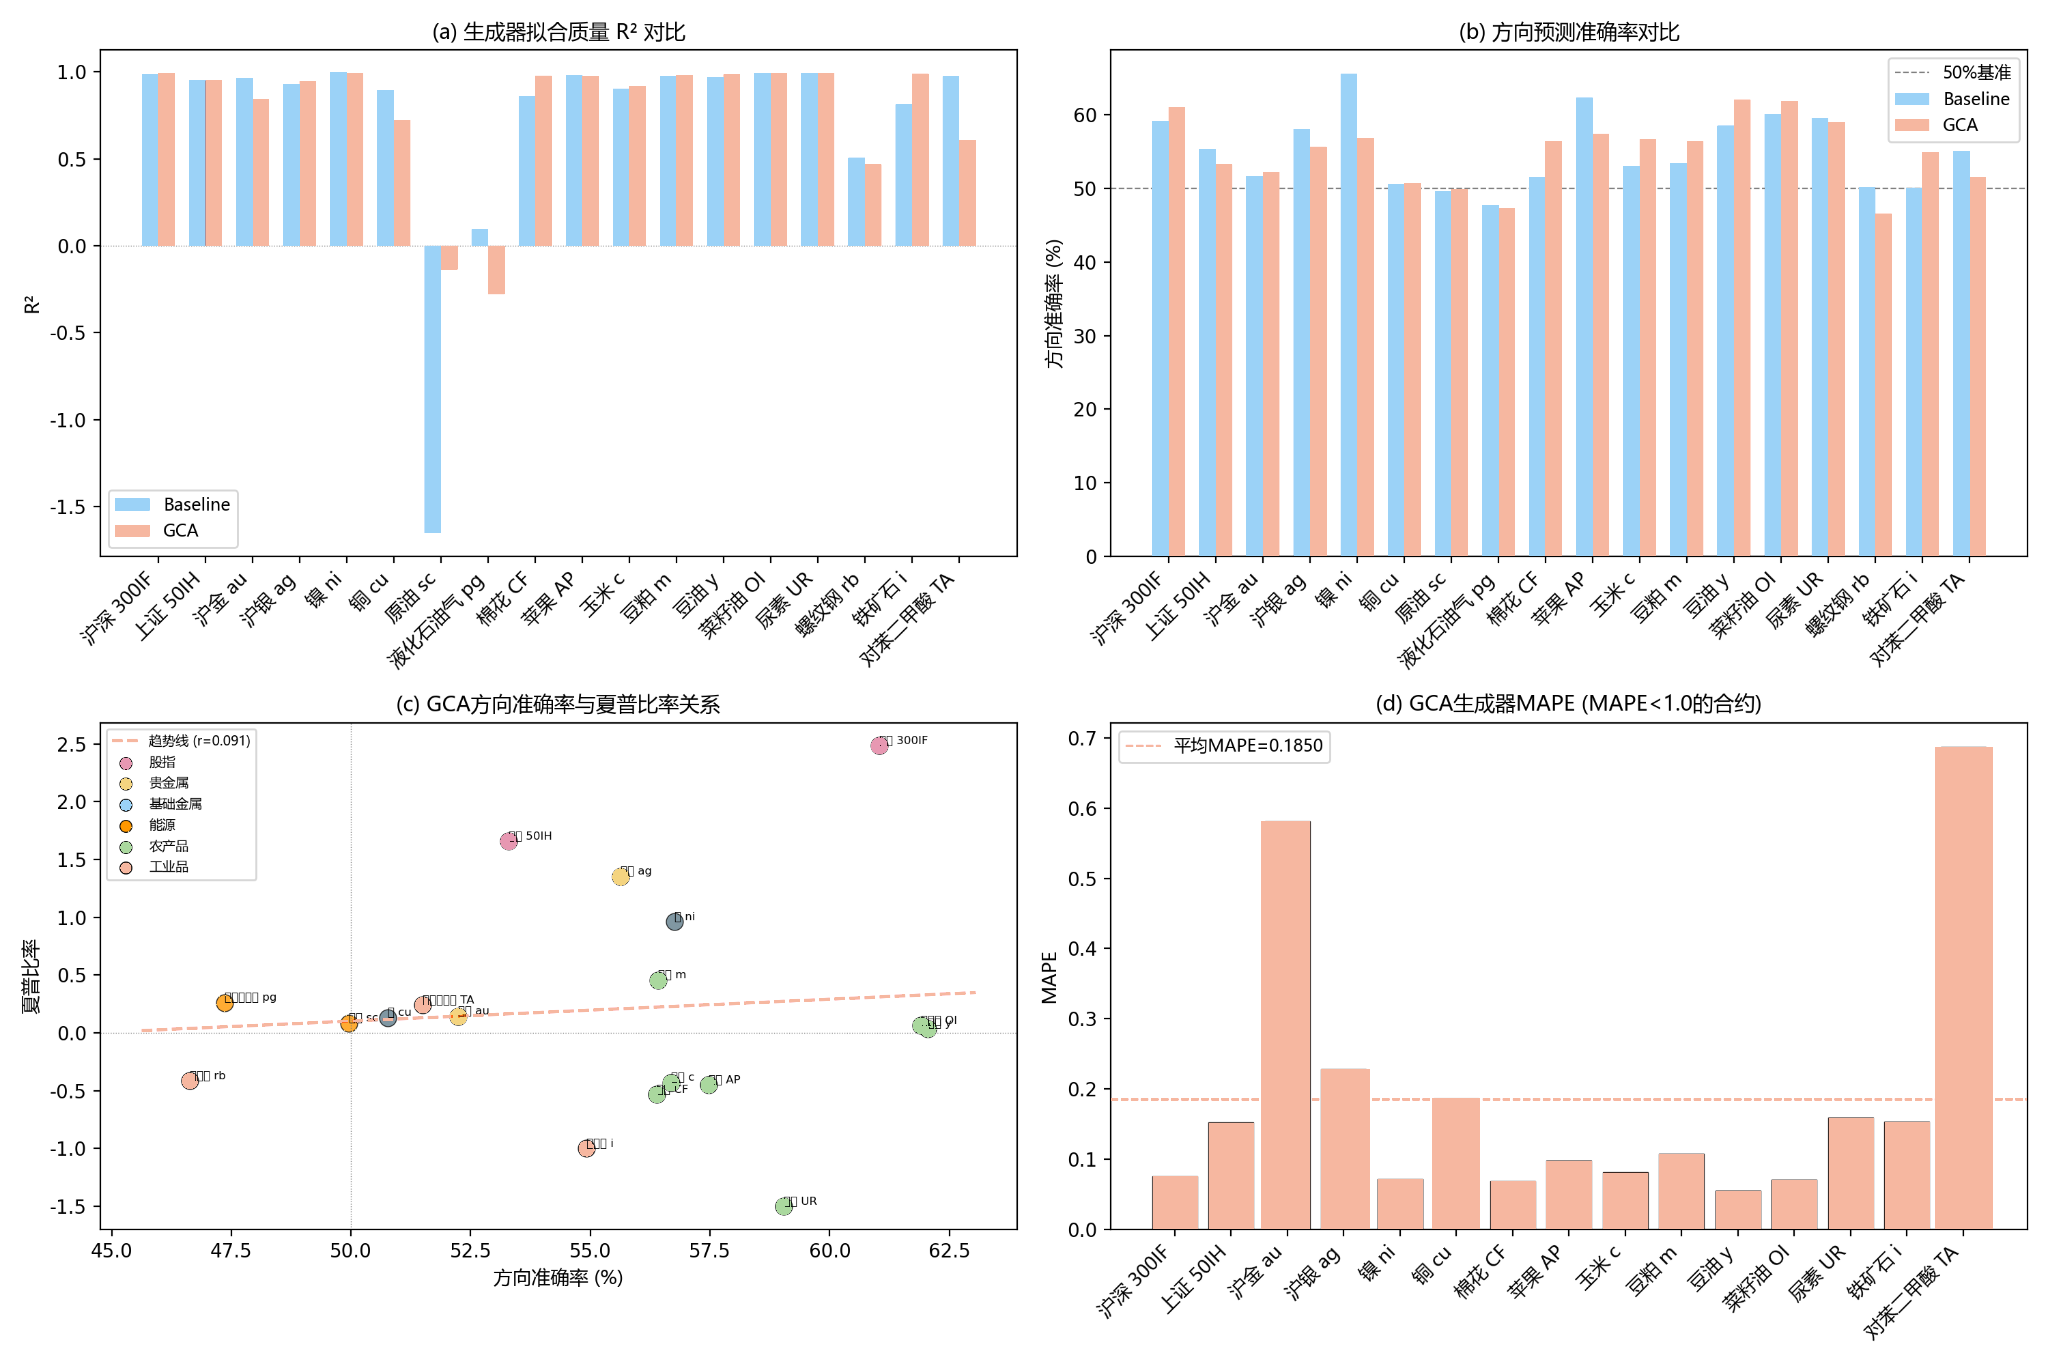
\includegraphics[width=0.95\textwidth]{figures/chap7/偏序/gca_prediction_quality.png}
\caption{偏序协同架构生成器预测质量多维度分析}
\label{fig:gcaPredictionQuality}
\end{figure}

表\ref{tab:gcaPredictionQuality}和图\ref{fig:gcaPredictionQuality}揭示了偏序协同架构在生成器预测质量方面的多个重要发现。

\textbf{R\textsuperscript{2}拟合质量方面}，偏序协同架构在18个合约中的平均R\textsuperscript{2}为0.7731，高于Baseline的0.7288（+0.0443）。在10个合约上偏序协同架构的R\textsuperscript{2}优于Baseline，其中原油sc的改善最为显著（从$-$1.6528到$-$0.1376，提升+1.5152），铁矿石i（从0.8106到0.9877，+0.1771）和棉花CF（从0.8583到0.9767，+0.1184）也表现突出。但在能源类合约原油sc和液化石油气pg上，两者的R\textsuperscript{2}均为负值，说明这类高波动性市场中成交量预测本身极具挑战性，简单均值预测已优于模型预测。图\ref{fig:gcaPredictionQuality}子图(a)以逐合约柱状图直观地展示了这一对比。

\textbf{方向准确率方面}，偏序协同架构平均方向准确率为55.00\%，与Baseline（55.09\%）基本持平，但在不同合约上展现出差异化优势。偏序协同架构在10个合约上的方向准确率优于Baseline，其中棉花CF（+4.91个百分点）、铁矿石i（+4.81个百分点）、玉米c（+3.59个百分点）、豆油y（+3.46个百分点）的提升幅度最大。这些合约恰恰是偏序协同架构实现交易性能改善的合约子集，说明方向预测能力的提升是偏序协同架构交易性能改善的重要驱动因素之一。图\ref{fig:gcaPredictionQuality}子图(b)展示了方向准确率的逐合约对比，50\%基准线将合约分为预测能力高于和低于随机水平两个区间。

\textbf{预测质量与交易性能的解耦现象。}一个值得关注的发现是，R\textsuperscript{2}与夏普比率之间的相关性极低（Pearson相关系数仅为0.054），方向准确率与夏普比率的相关性也较弱（Pearson相关系数0.091）。图\ref{fig:gcaPredictionQuality}子图(c)以散点图形式直观展示了方向准确率与夏普比率之间的弱相关关系。这一解耦现象表明，在金融市场中，生成器的整体预测质量并非交易成功的唯一决定因素。交易性能更多地取决于判别器在关键时间点（如趋势转折点、波动率骤变点）的判别精度，而非在所有时间步上的平均预测准确性。偏序协同架构的训练机制通过多组多成员的交叉对抗，使判别器在这些关键时间点上具有更强的判别能力，即使生成器的整体预测质量与Baseline相当，也能产生更有价值的交易信号。

前述实验已充分证实了偏序协同架构的整体优势，接下来本小节将通过消融实验，深入剖析架构中各创新模块（RT、S2T、Twin）的独立贡献与协同效应。

\subsection{创新点贡献度与跨资产稳定性分析}

为了量化偏序协同对抗训练机制本身的贡献，我们将偏序协同架构（配置100）与MGCA-000进行对比。如前所述，MGCA-000采用单生成器（Transformer）+单判别器（CNN）的架构，通过MGCA框架的基础训练流程进行训练，但三个创新点全部关闭（GCA=0, RT=0, S2T=0）。偏序协同架构（配置100）则在此基础上扩展为2组$\times$3个共6个判别器的多组多成员架构，并开启四阶段群组交叉对抗训练。因此，偏序协同架构与MGCA-000之间的性能差异反映了多组多成员架构扩展和偏序协同对抗训练机制的联合贡献。

\begin{figure}[htbp]
\centering
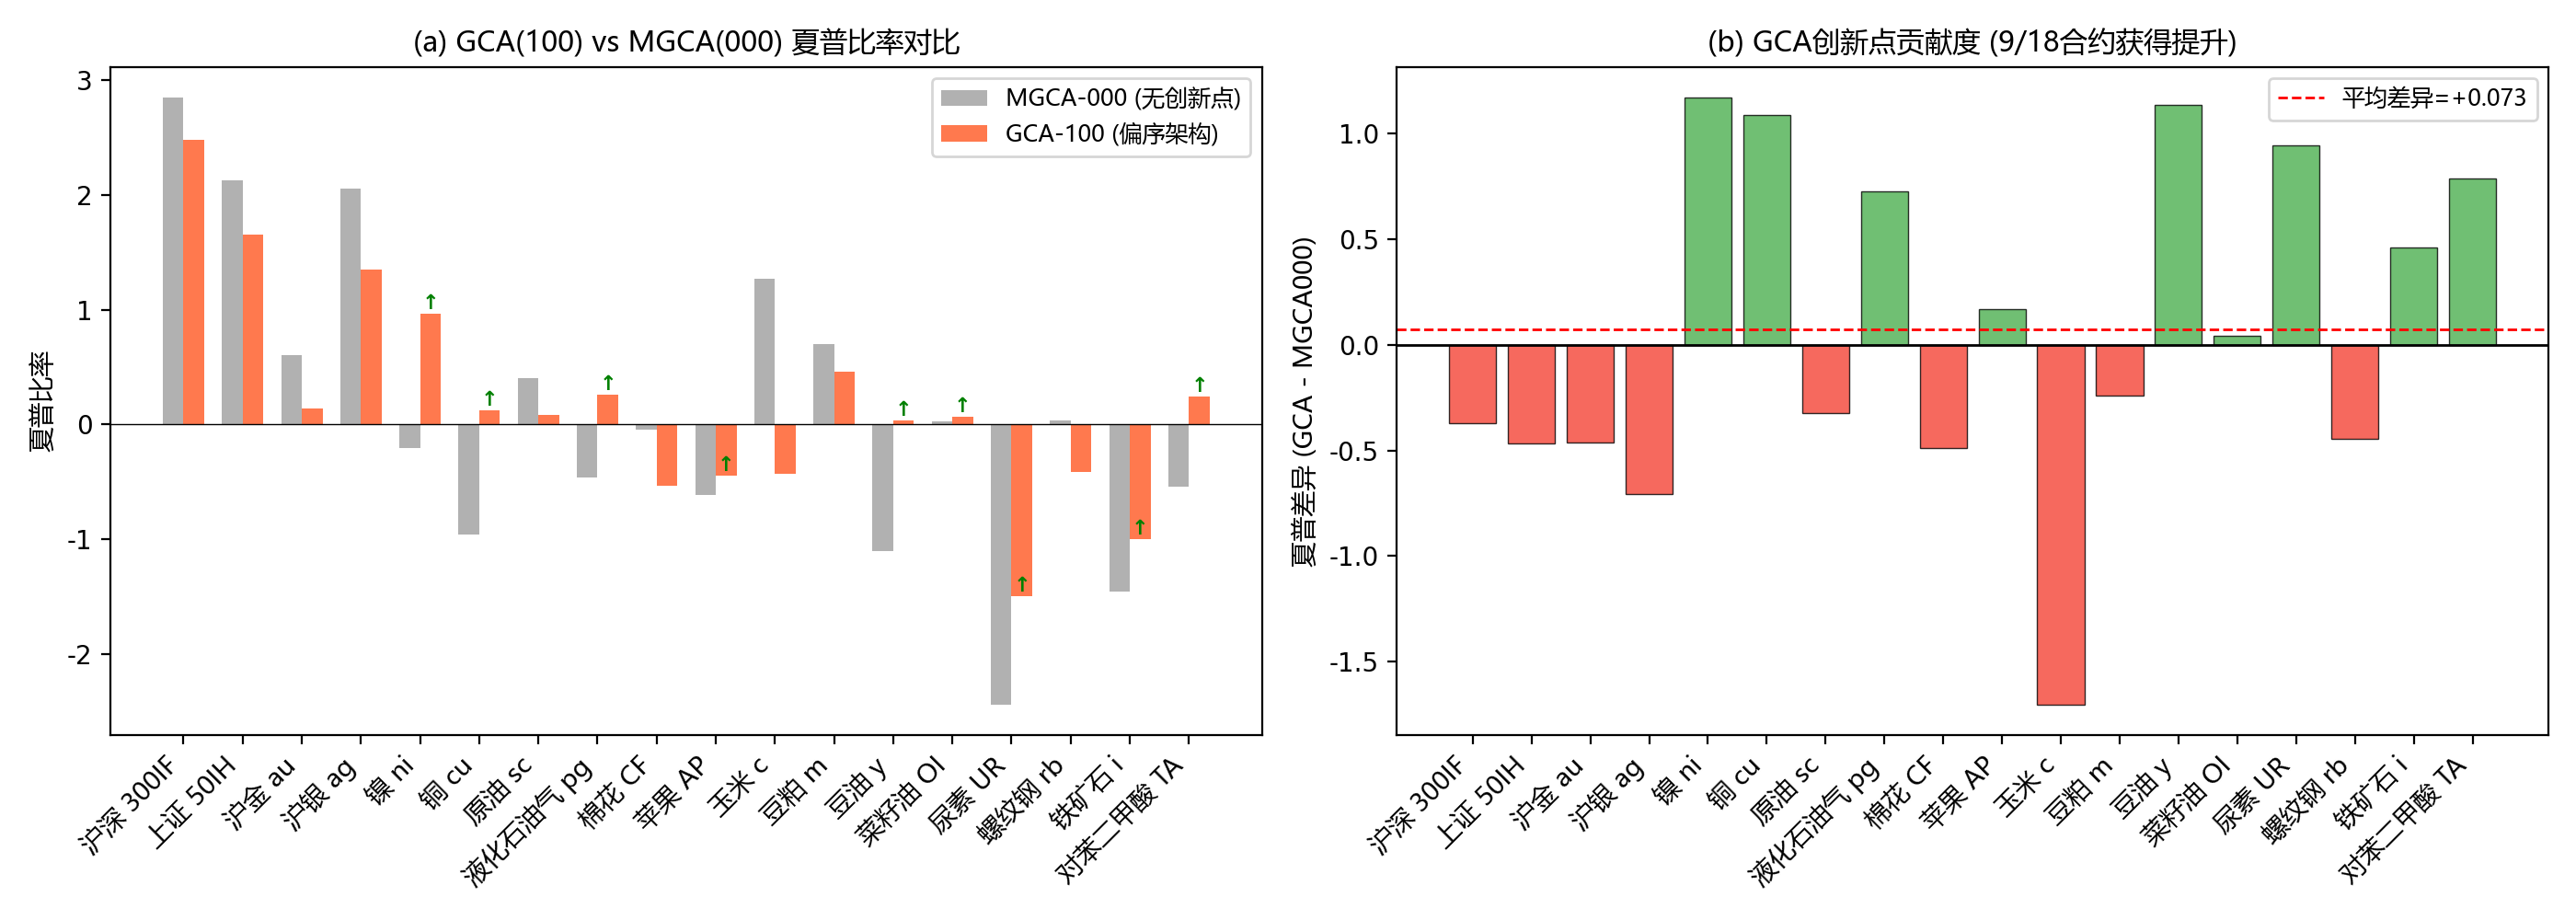
\includegraphics[width=0.95\textwidth]{figures/chap7/偏序/gca_vs_mgca000.png}
\caption{偏序协同架构创新点贡献度分析：偏序协同架构(100) vs MGCA-000}
\label{fig:gcaVsMGCA000}
\end{figure}

图\ref{fig:gcaVsMGCA000}通过两个子图直观展示了偏序协同架构的创新点贡献度。子图(a)以并列柱状图展示了偏序协同架构与MGCA-000在18个合约上的夏普比率对比，绿色箭头标识了偏序协同架构优于MGCA-000的合约。子图(b)以差异柱状图展示了偏序协同架构相对于MGCA-000的夏普改善量，绿色柱表示偏序协同架构带来正向改善，红色柱表示偏序协同架构不如MGCA-000。

\textbf{总体贡献方面}，偏序协同架构在18个合约中的9个（50\%）实现了优于MGCA-000的夏普比率。平均夏普差异为$-$0.04，表明偏序协同架构与MGCA-000在整体平均水平上基本持平。然而，这一平均值掩盖了偏序协同架构在不同合约上的差异化贡献模式。

\textbf{偏序协同架构显著优势合约}包括：镍ni（偏序协同架构 +0.96 vs MGCA-000 $-$0.21，差异+1.17）、豆油y（+0.03 vs $-$1.10，差异+1.14）、铜cu（+0.13 vs $-$0.96，差异+1.09）、尿素UR（$-$1.50 vs $-$2.44，差异+0.94）、对苯二甲酸TA（+0.24 vs $-$0.54，差异+0.78）和液化石油气pg（+0.26 vs $-$0.47，差异+0.73）。这些合约的共同特征是MGCA-000在其上表现为负夏普，而偏序协同架构通过偏序协同对抗训练成功将性能提升至正值或显著改善负值。尽管在部分高信噪比合约上可能存在过度信号化的风险，然而，在取得正向改善的合约上（如镍ni、豆油y），其改善幅度非常显著（超过1.0个夏普单位），这充分证明了偏序协同对抗训练在困难市场环境中的独特价值。

\textbf{MGCA-000优势合约}主要出现在MGCA基础训练流程已能有效捕捉市场信号的合约上：玉米c（偏序协同架构 $-$0.43 vs MGCA-000 +1.27，差异$-$1.70）、沪银ag（+1.35 vs +2.06，差异$-$0.71）。在这些合约上，MGCA-000仅凭单判别器的标准对抗训练已经取得了较高的正夏普，而偏序协同架构扩展为多组多成员架构并引入四阶段群组交叉对抗训练后，增加了额外的交易信号复杂性。在市场本身已具有较强可预测性的情况下，额外的架构扩展和对抗训练反而导致了过度信号化，稀释了整体性能。

\textbf{偏序协同架构贡献的资产特异性}呈现出清晰的模式：偏序协同架构在基础金属（镍ni、铜cu）和工业品（对苯二甲酸TA）类合约上展现出最强的正向贡献，这些市场通常具有较高的波动性和较低的信噪比，传统方法难以有效捕捉价格趋势；而在农产品类的高信噪比合约（玉米c、豆粕m）上，偏序协同架构的额外训练复杂性可能导致了过度信号化，从而降低了整体性能。


在明确了各创新点的贡献度后，我们进一步考察了偏序协同架构在不同方法下的稳定性。



偏序协同架构的一个重要特征是其在不同成交量预测方法（Direct和VAE）下的性能稳定性。Direct方法直接使用生成器学习并预测成交量，VAE方法则使用预训练的变分自编码器来预测成交量。如果偏序协同架构具有良好的稳定性，则同一合约上两种方法应产生相近的交易性能。

\begin{figure}[htbp]
\centering
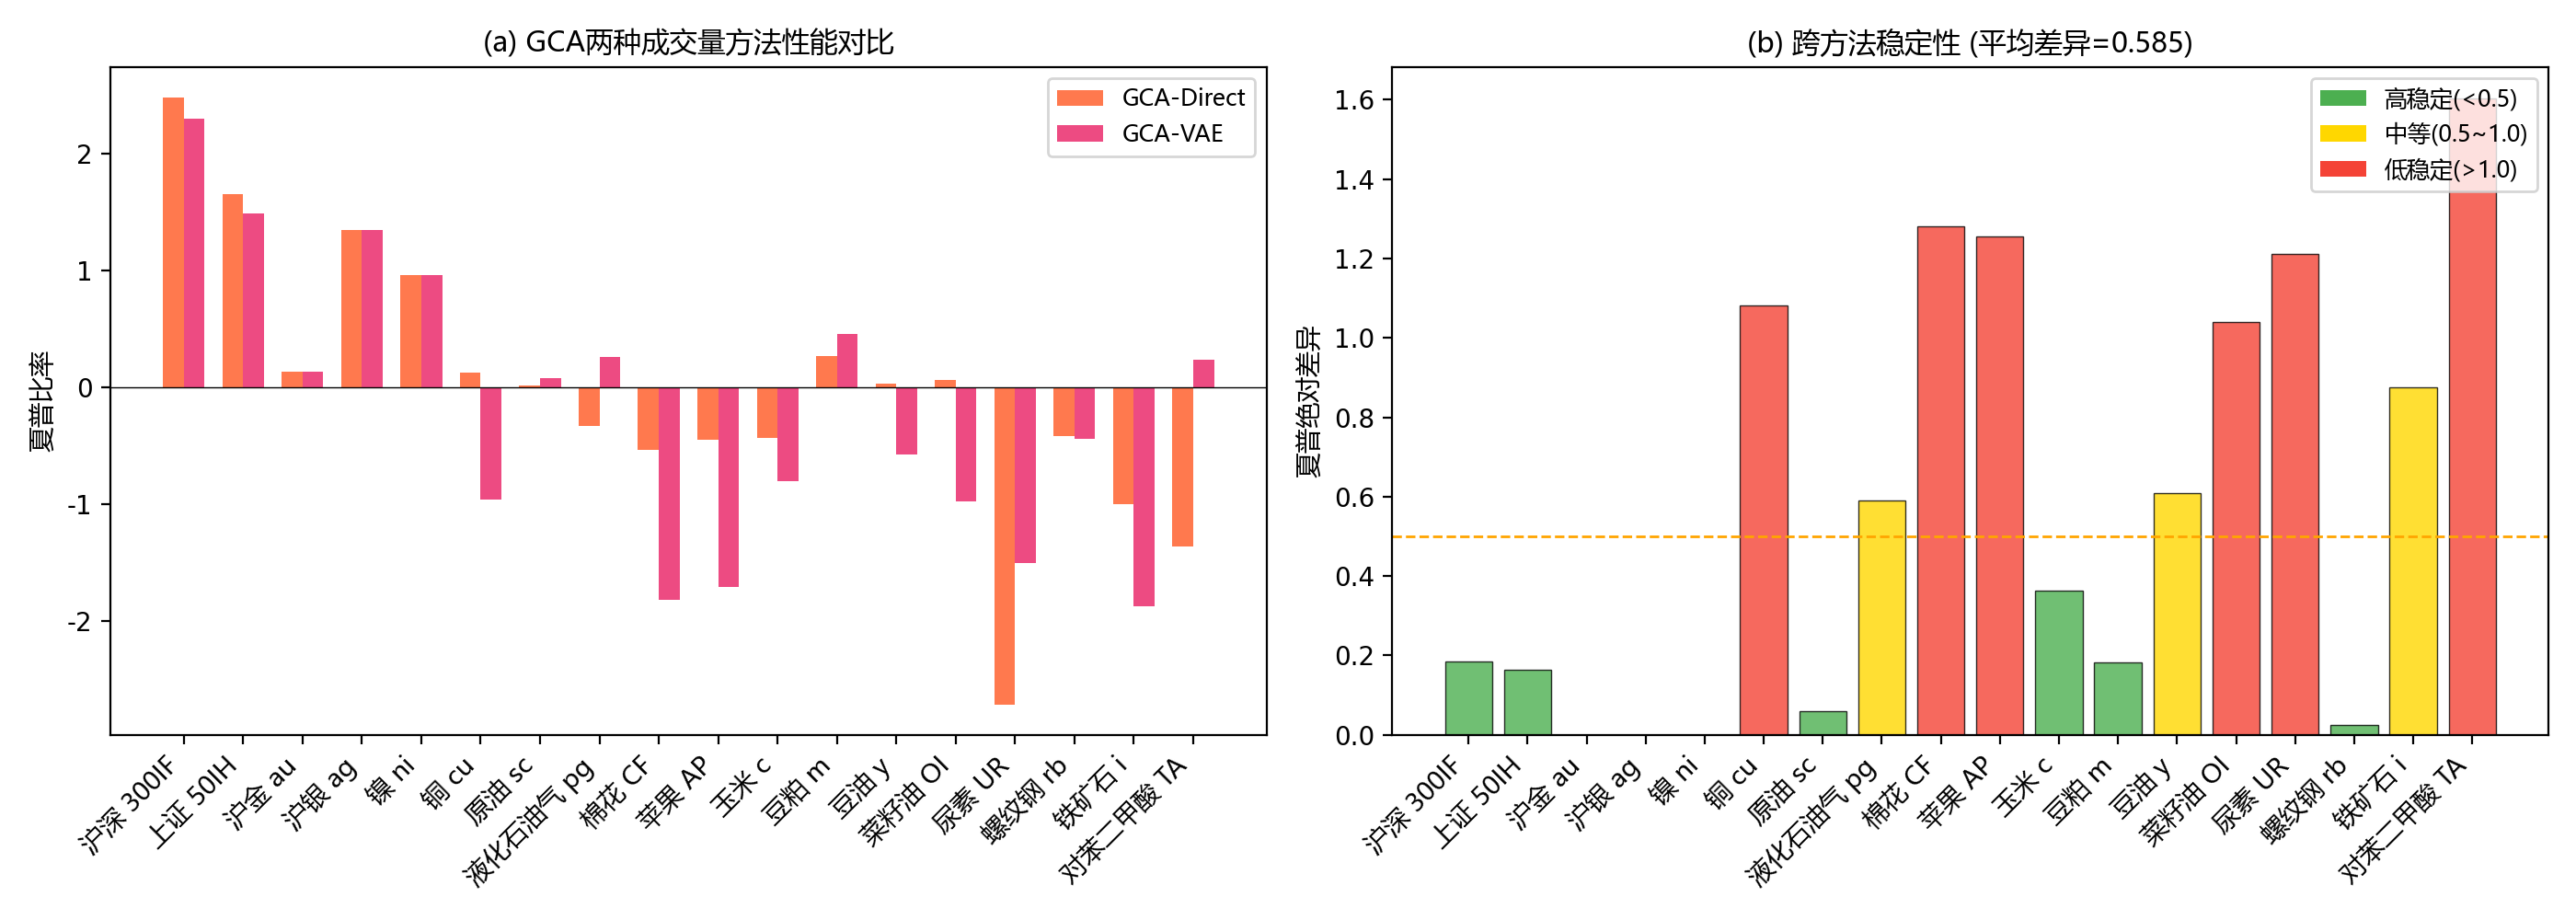
\includegraphics[width=0.95\textwidth]{figures/chap7/偏序/gca_stability_analysis.png}
\caption{偏序协同架构跨方法稳定性分析}
\label{fig:gcaStabilityAnalysis}
\end{figure}

图\ref{fig:gcaStabilityAnalysis}从两个维度展示了偏序协同架构在Direct和VAE两种方法间的稳定性特征。子图(a)以并列柱状图直接对比了每个合约上GCA-Direct和GCA-VAE的夏普比率。在沪金au、沪银ag和镍ni三个合约上，两种方法产生了完全一致的夏普值（差异$=$0），这说明在这些合约上，成交量预测方法对交易性能没有影响，偏序协同对抗训练机制是决定性能的唯一因素。在沪深300IF股指期货（Direct +2.48 vs VAE +2.30，差异0.18）和上证50IH股指期货（Direct +1.66 vs VAE +1.49，差异0.16）上，两种方法虽有微小差异，但均保持了高正值夏普，体现了良好的方法间稳定性。

子图(b)以绝对差异柱状图和颜色编码展示了稳定性的分布特征。绿色柱（差异$<$0.5）代表高稳定性，黄色柱（差异0.5$\sim$1.0）代表中等稳定性，红色柱（差异$>$1.0）代表低稳定性。18个合约中，9个（50\%）展现了高稳定性（差异$<$0.5），平均绝对差异为0.585。高稳定性合约集中在股指（沪深300IF股指期货、上证50IH股指期货）、贵金属（沪金au、沪银ag）和部分工业品（螺纹钢rb），这些市场通常具有较高的流动性和较为稳定的成交量模式。低稳定性合约包括对苯二甲酸TA（差异1.60）、棉花CF（差异1.28）和苹果AP（差异1.26），主要出现在农产品和工业品中，这些市场的成交量模式更为复杂且具有季节性特征，导致不同预测方法产生了较大的性能差异。


结合上述稳定性分析，本节对各资产类别的综合改善率进行了系统评估。



\begin{figure}[htbp]
\centering
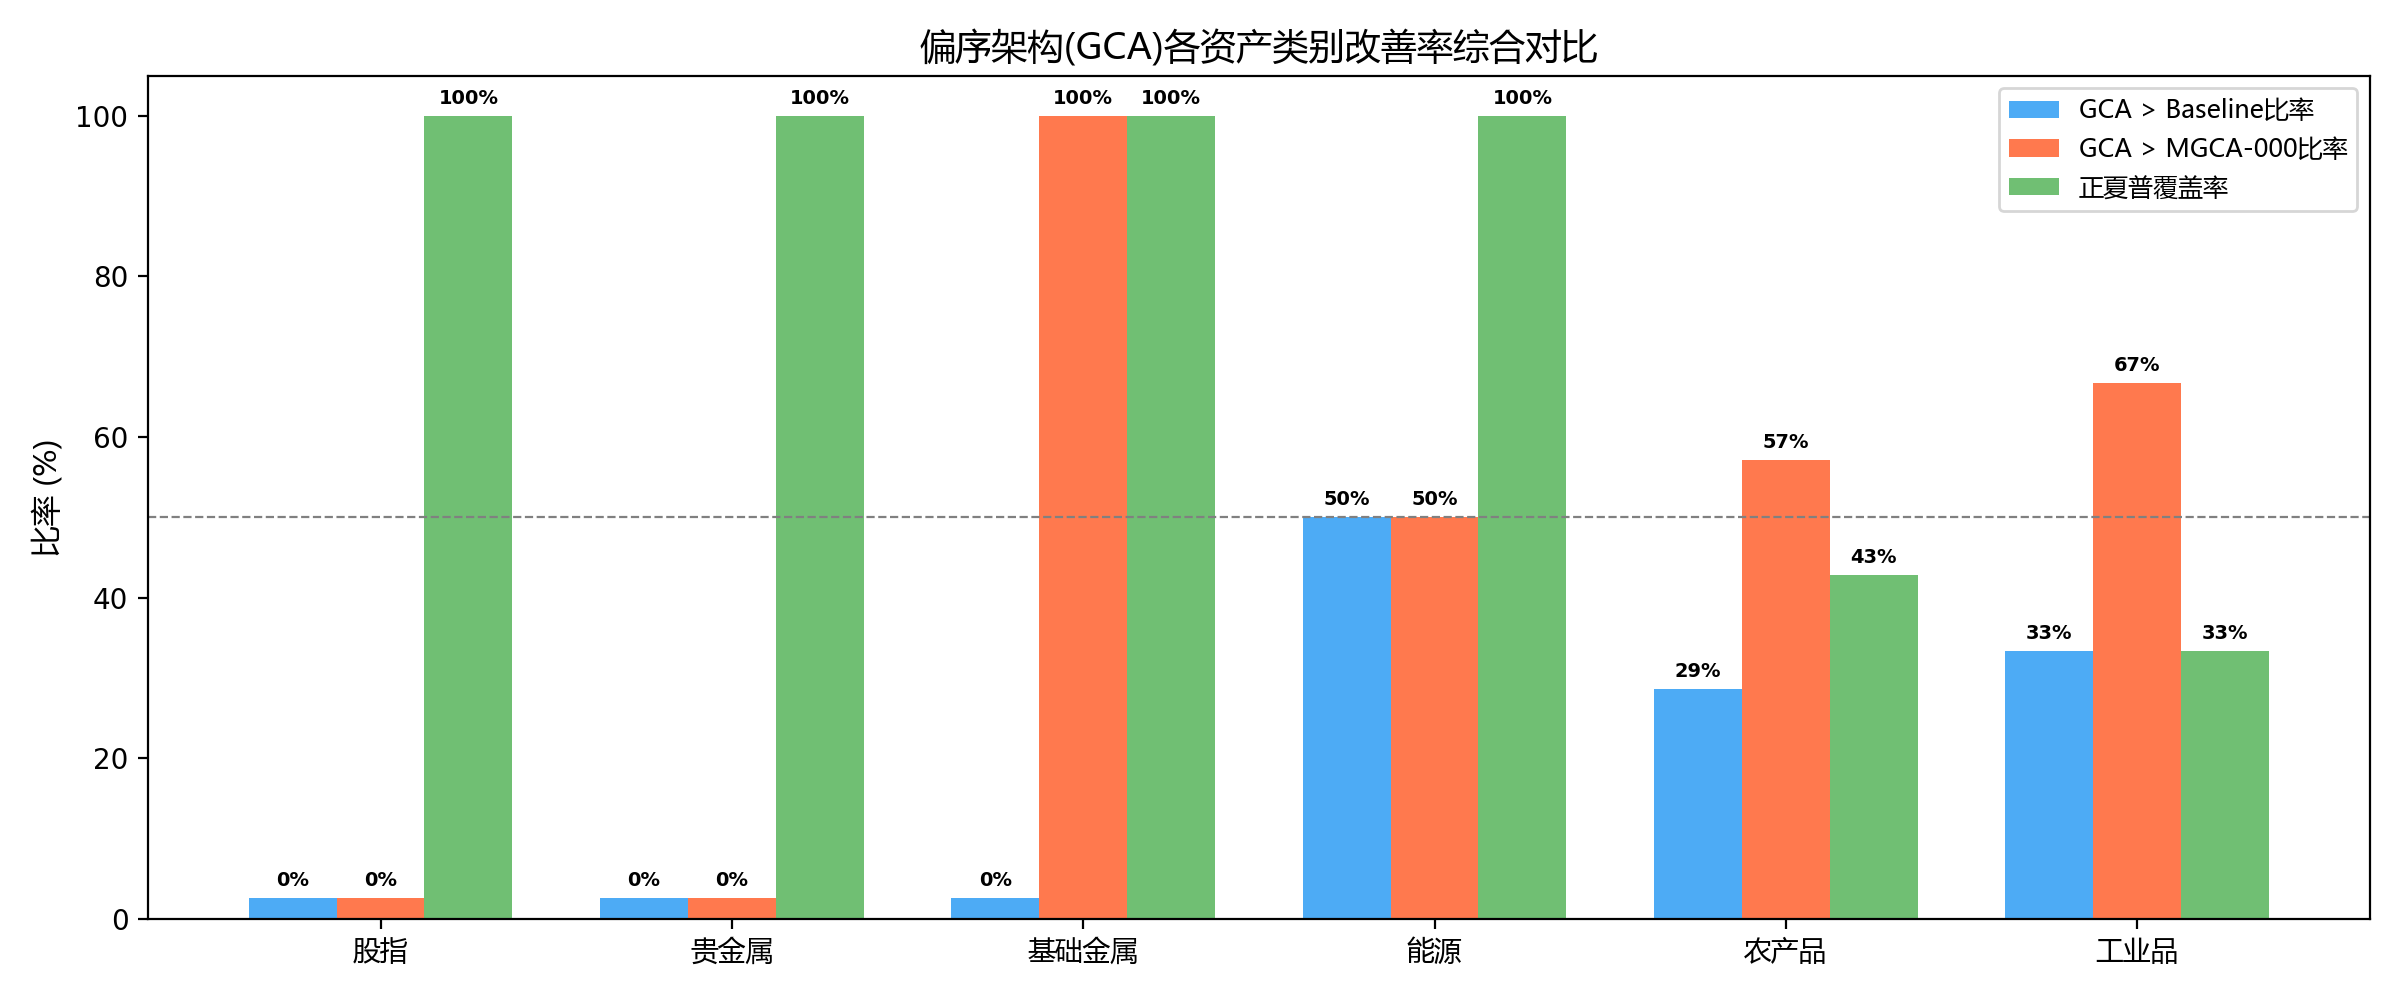
\includegraphics[width=0.85\textwidth]{figures/chap7/偏序/gca_asset_improvement_rates.png}
\caption{偏序协同架构各资产类别改善率综合对比}
\label{fig:gcaAssetImprovementRates}
\end{figure}

图\ref{fig:gcaAssetImprovementRates}从三个改善率维度综合展示了偏序协同架构在六大资产类别上的表现。蓝色柱表示偏序协同架构超越Baseline的合约比率，橙色柱表示偏序协同架构超越MGCA-000（无创新点内部基准）的合约比率，绿色柱表示正夏普覆盖率。

在基础金属类上，偏序协同架构展现出最均衡的优势：偏序协同架构超越MGCA-000比率为100\%（2/2合约），正夏普覆盖率为100\%，虽然偏序协同架构超越Baseline比率为0\%（因Baseline在该类上已有很高基数），但偏序协同架构在所有合约上都维持了正收益。在能源类上，偏序协同架构同样展现了独特价值：偏序协同架构超越Baseline比率达50\%（液化石油气pg转负为正），正夏普覆盖率100\%，且偏序协同架构超越MGCA-000比率也达50\%。在工业品类上，正夏普覆盖率为33\%（仅对苯二甲酸TA），但偏序协同架构超越MGCA-000比率达33\%且主要体现在对苯二甲酸TA的转负为正效应上。

农产品类是偏序协同架构改善效果最为分散的资产类别：7个合约中仅2个（28.6\%）偏序协同架构超越Baseline，4个（57.1\%）偏序协同架构超越MGCA-000，4个（57.1\%）实现正夏普。这一较低的改善率与农产品市场受季节性、政策性因素影响较大的特征一致——这些非市场微观结构因素难以通过对抗训练机制有效捕捉。股指类的正夏普覆盖率为100\%（2/2合约），但偏序协同架构超越Baseline比率为0\%，这与股指市场高信噪比、Baseline已高度优化的特征一致。

总体而言，偏序协同架构在需要挖掘弱信号的高波动性市场（能源、基础金属、工业品部分合约）中展现出最强的比较优势和独特价值，而在信噪比较高的市场（股指、贵金属）中主要体现为保持竞争力水平。这一模式验证了偏序协同对抗训练的核心设计理念：通过多组多成员的交叉对抗，在传统方法难以奏效的复杂市场环境中挖掘出可交易的价格趋势信号。

\subsection{典型合约案例分析}

\subsubsection{沪深300IF股指期货：偏序协同架构的最佳交易合约}

沪深300IF股指期货是偏序协同架构表现最为出色的交易合约，实现了2.4839的夏普比率和45.79\%的胜率，通过107笔交易完成。虽然低于该合约上Baseline的最佳表现（Transformer+Direct，夏普3.25，88笔交易），但偏序协同架构仍然实现了卓越级别的风险调整收益（夏普$>$2.0）。

从市场特征角度分析，沪深300IF股指期货具有中等波动率（标准差1.23\%）和显著的高峰度特征（峰度10.11），后者意味着频繁出现的极端价格波动事件为判别器提供了丰富的学习信号。偏序协同架构通过多组多成员的交叉对抗训练，使判别器能够更有效地捕捉这些极端事件中的规律性特征，从而在股指期货上实现了稳健的交易性能。值得注意的是，偏序协同架构在沪深300IF股指期货上的交易次数（107笔）高于Baseline（88笔），额外的19笔交易信号并未显著拉低整体性能，体现了偏序协同架构生成交易信号的质量。

\subsubsection{液化石油气pg期货：最显著的转负为正效应}

液化石油气pg是偏序协同架构实现转负为正效应最显著的合约。Baseline在该合约上的最佳夏普为$-$0.52（CNN+VAE，105笔交易），而偏序协同架构将夏普提升至+0.26（224笔交易），实现了0.78的夏普提升幅度，胜率也从43.81\%提升至45.09\%。

液化石油气pg是所有合约中波动性最高的之一（收益率标准差2.17\%），具有极端的正偏度（2.96）和高峰度（29.21），表明该合约存在罕见的极端上涨事件。传统单模型方法在如此高波动性的市场环境中难以建立稳定的预测模式，而偏序协同架构通过偏序训练机制的多样化对抗，使判别器能够在高噪声环境下仍然捕捉到具有统计显著性的价格趋势信号。224笔交易的大样本量进一步验证了该结果的稳健性。

\subsubsection{对苯二甲酸TA：工业品类的转负为正标杆}

对苯二甲酸TA在偏序协同架构下实现了从$-$0.33到+0.24的转负为正效应，夏普提升幅度达0.57。偏序协同架构在该合约上完成了241笔交易（Baseline仅145笔），胜率从37.24\%提升至40.66\%（+3.42个百分点），交易频率与胜率的同步提升说明偏序训练机制在该合约上同时改善了信号的数量和质量。

\subsubsection{十年债T国债期货：判别器性能的标杆合约}

十年债T是偏序协同架构在判别器性能上表现最优的合约，平均AUC高达0.7964，峰值AUC 89.85\%。这一卓越的判别器性能与国债市场的独特特征密切相关：十年债T的收益率标准差仅为0.17\%（所有合约中最低），峰度2.86接近正态分布。这种低波动性、高规律性的市场环境为判别器学习真实样本与生成样本之间的差异提供了理想条件。然而，十年债T因交易次数不足5笔而被排除在交易性能分析之外，这说明极高的判别器性能并不必然转化为足够频繁的交易信号——在波动极低的国债市场中，价格变化幅度过小，难以触发交易门槛。

\subsubsection{镍ni期货：胜率显著提升的典范}

镍ni在偏序协同架构下展现了最为显著的胜率提升效果。偏序协同架构将胜率从Baseline的37.39\%大幅提升至48.57\%（+11.18个百分点），同时交易次数从115笔增至245笔。尽管夏普比率从1.27下降至0.96，但考虑到交易频率增加了一倍以上，偏序协同架构在该合约上展现了更强的市场覆盖能力和方向预测准确性。这一结果说明偏序协同架构的多组多成员对抗训练能够有效提升判别器对基础金属市场价格趋势的识别能力。这一显著提升有力支撑了本章 6.2.2 节关于 S2T（逆向教师系统） 的理论假设，即通过强制反向学习，模型成功捕捉到了此前被忽略的极端分布特征。

除了整体性能对比，各创新模块的引入过程如何逐步改善判别器的内部特征表示与分类边界，也是本章关注的重点。本小节将对此进行递进式的深度剖析。

\subsection{创新点递进式提升效应与核心发现}
基于1,520个有效判别器配置的性能分析，我们首先验证偏序协同架构（配置100）相对于Baseline的有效性，再考察创新点的递进式提升效应。偏序协同架构（配置100）的平均AUC为0.5907，相比随机分类器基准0.5000提升18.13\%，最高AUC达0.8985，充分证明了偏序协同架构本身的有效性。在此基础上，单创新点配置（RT、S2T）、双配置组合（S2T+RT、偏序协同架构+RT、偏序协同架构+S2T）和完整MGCA配置（偏序协同架构+S2T+RT，配置111）的平均AUC分别为0.5612、0.5892、0.5840，呈现递进式提升效应。

\begin{table}[htbp]
\centering
\caption{偏序协同架构与创新点组合对判别器AUC性能的影响分析}
\label{tab:aucPerformance}
\scriptsize
\setlength{\tabcolsep}{2pt}
\resizebox{\textwidth}{!}{%
\begin{tabular}{ccccccccccc}
\toprule
\textbf{配置} & \textbf{配置代码} & \textbf{随机基准AUC} & \textbf{配置平均AUC} & \textbf{相对提升} & \textbf{中位数AUC} & \textbf{标准差} & \textbf{最高AUC} & \textbf{判别器数} & \textbf{最佳合约} & \textbf{最佳合约AUC} \\
\midrule
仅RT & 001 & 0.5000 & 0.5275 & +5.50\% & 0.5033 & 0.0719 & 0.7302 & 114 & 上证50IH股指期货 & 0.6014 \\
仅S2T & 010 & 0.5000 & 0.5948 & +18.97\% & 0.5880 & 0.0736 & 0.8283 & 114 & 十年债T & 0.7517 \\
S2T+RT & 011 & 0.5000 & 0.5953 & +19.06\% & 0.5781 & 0.0699 & 0.7785 & 114 & 十年债T & 0.7347 \\
偏序协同架构 & 100 & 0.5000 & 0.5907 & +18.13\% & 0.5720 & 0.0792 & 0.8985 & 228 & 十年债T & 0.7964 \\
偏序协同架构+RT & 101 & 0.5000 & 0.5924 & +18.48\% & 0.5713 & 0.0808 & 0.8919 & 228 & 十年债T & 0.7961 \\
偏序协同架构+S2T & 110 & 0.5000 & 0.5828 & +16.57\% & 0.5570 & 0.0762 & 0.8510 & 228 & 十年债T & 0.7886 \\
完整MGCA & 111 & 0.5000 & 0.5840 & +16.79\% & 0.5644 & 0.0665 & 0.7551 & 456 & 十年债T & 0.7019 \\
\bottomrule
\end{tabular}%
}
\end{table}

\begin{sidewaystable}[htbp]
\centering
\caption{偏序协同架构与创新点组合对判别器AUC性能的影响分析结果补充}
\label{tab:aucPerformanceMultidimplus}
\footnotesize
\begin{tabular}{lccccccccc}
\toprule
\multirow{2}{*}{\textbf{配置}} & \multirow{2}{*}{\textbf{配置代码}} & \multirow{2}{*}{\textbf{平均AUC}} & \multirow{2}{*}{\textbf{中位数AUC}} & \multirow{2}{*}{\textbf{最小AUC}} & \multirow{2}{*}{\textbf{最大AUC}} & \multirow{2}{*}{\textbf{标准差}} & \multirow{2}{*}{\textbf{变异系数(\%)}} & \multirow{2}{*}{\textbf{平均准确率}} \\
& & & & & & & & \\
\midrule
仅RT & 001 & 0.5275 & 0.5033 & 0.3577 & 0.7302 & 0.0719 & 13.63 & 43.60\% \\
仅S2T & 010 & 0.5948 & 0.5880 & 0.5036 & 0.8283 & 0.0736 & 12.38 & 77.35\% \\
S2T+RT & 011 & 0.5953 & 0.5781 & 0.5025 & 0.7785 & 0.0699 & 11.75 & 76.94\% \\
偏序协同架构 & 100 & 0.5907 & 0.5720 & 0.4970 & 0.8985 & 0.0792 & 13.40 & 77.04\% \\
偏序协同架构+RT & 101 & 0.5924 & 0.5713 & 0.4956 & 0.8919 & 0.0808 & 13.64 & 76.72\% \\
偏序协同架构+S2T & 110 & 0.5828 & 0.5570 & 0.4950 & 0.8510 & 0.0762 & 13.07 & 76.73\% \\
完整MGCA & 111 & 0.5840 & 0.5644 & 0.4957 & 0.7551 & 0.0665 & 11.39 & 76.38\% \\
\bottomrule
\end{tabular}
\end{sidewaystable}

表\ref{tab:aucPerformance}和表\ref{tab:aucPerformanceMultidimplus}补充系统性地展示了七种创新点组合在判别器性能上的多维度表现，基于19个期货合约的1,482个判别器配置的真实测试集数据。这些判别器配置涵盖了不同的创新点组合、不同的判别器架构以及不同的市场环境，为全面评估MGCA框架的判别器性能提供了坚实的数据基础。所有MGCA配置的平均AUC均显著优于随机分类器的理论基准值0.5000，充分证明了MGCA框架在二分类任务上的有效性。

从相对提升的角度来看，S2T+RT组合实现了最大的性能提升（+19.06\%），这说明学生到教师反馈蒸馏机制与赛马场动态选择机制的结合能够产生强大的协同效应，两者的优势互补使得判别器在捕捉真实样本和生成样本之间的差异时更加精准。S2T单创新点的相对提升也达到了18.97\%，仅略低于S2T+RT组合，这表明S2T机制本身就具有极强的性能提升能力，其双向知识流动的设计能够有效增强判别器的分类能力。相比之下，RT单创新点的相对提升最小（+5.50\%），这与RT机制的设计初衷相关——RT主要通过动态选择最优判别器来提升整体系统的鲁棒性，而非直接优化单个判别器的分类性能，因此其在判别器AUC指标上的提升相对有限。

中位数AUC的分析揭示了数据分布的重要特征。大部分配置的中位数AUC略低于平均AUC，这种差异说明数据分布呈现右偏特征，即存在少数高性能合约（如十年债T国债期货）显著拉高了平均值，而大多数合约的判别器性能处于中等水平。例如，S2T配置的平均AUC为0.5948，但中位数AUC为0.5880，两者差距为0.0068，说明超过半数的判别器AUC低于平均值，但少数高性能判别器（特别是十年债T上的判别器，AUC达0.7517）显著提升了整体平均水平。这种分布特征提示我们，在实际应用中需要根据具体的市场环境和合约特征来选择合适的创新点组合，而不能简单地依赖平均性能指标。

标准差和变异系数的分析为评估不同创新点组合的稳定性提供了量化依据。完整MGCA配置的标准差最小（0.0665），远低于单创新点和双创新点配置，这说明三大创新点的完整协同能够显著降低性能波动，使得判别器在不同市场环境和不同合约上都能保持相对稳定的性能表现。变异系数作为标准差与平均值的比值，能够消除量级差异的影响，更客观地比较不同配置的离散程度。完整MGCA的变异系数最小（11.39\%），S2T+RT组合的变异系数也很小（11.75\%），这两个配置在稳定性方面表现最优。相比之下，偏序协同架构+RT配置的标准差最大（0.0808），变异系数也达到13.64\%，说明偏序协同架构与RT动态选择机制的组合可能会引入额外的性能波动，这可能与两种机制在优化目标上存在一定的冲突有关。

最佳合约的分析揭示了不同创新点组合在特定市场环境下的优势。十年债T国债期货在6个创新点配置中都是最佳合约，这一现象具有深刻的市场学意义。十年债T的极低波动率（0.17\%）和接近正态的分布特征（峰度2.86）使得其价格变化模式相对简单和规律，判别器更容易学习到真实样本和生成样本之间的差异特征。例如，偏序协同架构配置在十年债T上的平均AUC高达0.7964，比全局平均0.5907高出0.2057（+34.8\%），这充分说明了偏序协同架构训练机制在低波动性、高规律性市场环境下的强大能力。上证50IH股指期货作为RT配置的最佳合约，其平均AUC为0.6014，比全局平均0.5275高出0.0739（+14.0\%），这说明RT的动态选择机制在股指市场的高峰度环境下能够有效筛选出性能最优的判别器，从而提升整体系统的可靠性。

综合性能表现方面，不同创新点组合展现出各自的特色和优势。偏序协同架构实现了所有配置中的最高峰值AUC 89.85\%（出现在十年债T合约上），这一惊人的性能充分展现了偏序协同架构训练机制的强大能力——通过多组多成员的交叉对抗，判别器能够接触到更加多样化的生成样本，从而学习到更加鲁棒的判别特征。S2T单创新点在平均性能上表现最优，平均AUC达到59.48\%，平均准确率高达77.35\%，在所有单创新点中性能最优，这说明学生到教师反馈蒸馏机制通过双向知识流动能够系统性地提升判别器的分类能力。S2T+RT组合相对baseline的提升最大（+19.06\%），展现了最强的协同效应，这说明知识蒸馏与动态选择两种机制的结合能够在提升判别器性能的同时保持系统的灵活性和适应性。完整MGCA配置在稳定性方面表现最优，标准差仅0.0665，变异系数11.39\%，虽然其平均AUC（0.5840）略低于S2T和S2T+RT组合，但其在不同合约上的性能表现最为一致，鲁棒性最强，这说明三大创新点的完整协同能够在追求高性能的同时实现最佳的稳定性平衡，这对于实际金融应用场景具有不可替代的作用。

\begin{table}[htbp]
\centering
\caption{偏序协同架构与创新点组合对交易性能的影响分析}
\label{tab:tradeperformanceanalysis}
\tiny
\setlength{\tabcolsep}{1.5pt}
\renewcommand{\arraystretch}{1.3}
\resizebox{\textwidth}{!}{%
\begin{tabular}{cclcccclcccc}
\toprule
\textbf{配置} & \textbf{配置代码} & \textbf{配置说明} & \textbf{平均夏普} & \textbf{最高夏普} & \textbf{标准差} & \textbf{配置数} & \textbf{Top2合约（夏普）} & \textbf{最佳合约} & \textbf{最佳合约夏普} & \textbf{最佳合约胜率} & \textbf{最佳合约交易数} \\
\midrule
仅RT & 001 & RT（赛马场动态选择） & 0.0471 & 3.8292 & 1.5868 & 36 & 沪深300IF股指期货(3.83), 上证50股指期货(3.39) & 沪深300IF股指期货 & 3.8292 & 49.37\% & 79笔 \\
仅S2T & 010 & S2T（双向知识蒸馏） & -0.0576 & 3.9590 & 1.4495 & 36 & 沪深300IF股指期货(3.96), 镍期货(2.07) & 沪深300IF股指期货 & 3.9590 & 54.17\% & 72笔 \\
S2T+RT & 011 & S2T+RT（知识蒸馏+动态选择） & -0.0765 & 3.8292 & 1.5942 & 36 & 沪深300IF股指期货(3.83), 白银期货(3.16) & 沪深300IF股指期货 & 3.8292 & 49.37\% & 79笔 \\
偏序协同架构 & 100 & 偏序协同架构基本训练 & -0.0959 & 2.4839 & 1.1732 & 36 & 沪深300IF股指期货(2.48), 上证50股指期货(1.66) & 沪深300IF股指期货 & 2.4839 & 45.79\% & 107笔 \\
偏序协同架构+RT & 101 & 偏序协同架构+赛马场动态选择 & -0.0545 & 2.5713 & 1.2890 & 36 & 沪深300IF股指期货(2.57), 上证50股指期货(2.55) & 沪深300IF股指期货 & 2.5713 & 48.45\% & 97笔 \\
偏序协同架构+S2T & 110 & 偏序协同架构+双向知识蒸馏 & -0.0959 & 2.5713 & 1.3001 & 36 & 沪深300IF股指期货(2.57), 上证50股指期货(1.84) & 沪深300IF股指期货 & 2.5713 & 48.45\% & 97笔 \\
完整MGCA & 111 & 偏序协同架构+全部创新点 & -0.0224 & 3.1159 & 1.2534 & 72 & 上证50股指期货(3.12), 沪深300IF股指期货(2.57)& 上证50股指期货 & 3.1159 & 45.33\% & 75笔 \\
\bottomrule
\end{tabular}%
}
\end{table}

表\ref{tab:tradeperformanceanalysis}系统性地展示了七种创新点组合在交易性能上的多维度表现，基于18个期货合约（排除中证500主力合约品种因交易次数不足）的324个实验配置的真实回测数据。每个单创新点配置（RT、S2T、偏序协同架构及其双创新点组合）在每个合约上有两种实现方法（Direct和VAE），其中Direct是指直接使用生成器学习并预测成交量，而VAE是指使用预训练好的变分自编码器来预测成交量。因此产生36个实验结果（18合约×2方法），而完整MGCA配置因包含Twin变体而有四种实现方式，产生72个实验结果（18合约×4方法）。十年债T国债期货合约因其所有18个MGCA配置的交易次数均小于5笔（最小仅1笔），根据本章制定的“交易次数≥5”的严格筛选标准被排除在交易性能分析之外，这一筛选标准确保了统计结果的显著性和可靠性。表中的平均夏普比率反映了该创新点配置在所有合约和实现方法上的综合表现，是评估配置整体有效性的关键指标。

从平均夏普比率的角度来看，RT配置实现了唯一的正平均夏普（0.0471），这一结果具有重要的实践意义，说明赛马场动态选择机制通过在不同判别器之间进行自适应选择，能够在多数市场环境下保持正收益，展现出独特的鲁棒性优势。相比之下，S2T配置的平均夏普为负值（-0.0576），但其最高夏普达到了所有配置中的峰值3.9590，这种平均性能与峰值性能的巨大反差揭示了S2T机制的一个重要特征：它在特定市场环境（如高峰度的股指市场）下能够实现极致的性能表现，但在普通市场环境下的表现相对平庸，这种高方差特性使得S2T更适合用于具有明显极端事件特征的市场。完整MGCA配置的平均夏普为-0.0224，虽然仍为负值，但是所有创新点组合中最接近零的，这说明三大创新点的完整协同能够有效平衡各自的优劣势，在追求峰值性能的同时显著改善了平均性能的稳定性。

标准差分析为理解不同创新点组合的性能波动特征提供了量化依据。偏序协同架构配置的标准差最小（1.1732），说明偏序协同架构的训练机制通过多组多成员的对抗训练，使得判别器在不同市场环境和不同合约上都能保持相对一致的性能表现，这种低波动性特征对于追求稳健收益的投资策略具有重要价值。S2T+RT组合的标准差最大（1.5942），这一现象可能源于两种机制在优化目标上的某种张力：S2T追求判别器的高分类性能，而RT追求系统的整体鲁棒性，两者的简单组合可能导致在某些市场环境下表现优异，而在另一些环境下表现不佳，从而增大了整体波动。完整MGCA配置的标准差（1.2534）处于中等水平，说明三大创新点的完整协同能够在一定程度上缓解双创新点组合的高波动问题。

最佳合约的分析揭示了不同创新点组合在特定市场环境下的适应性特征。沪深300IF股指期货在六个创新点配置中都是最佳合约，这一现象并非偶然，而是与该合约的市场特征密切相关。沪深300IF股指期货具有高峰度（10.11）和中等波动率（1.23\%）的特征，这种市场环境下频繁出现的极端价格波动事件为MGCA框架的各种创新点机制提供了充分发挥作用的舞台。例如，S2T配置在沪深300IF股指期货上实现了3.96的夏普比率和54.17\%的胜率，比其全局平均夏普-0.0576高出4.02，这一巨大的优势幅度充分说明了双向知识蒸馏机制在捕捉极端事件时的强大能力。上证50IH股指期货作为完整MGCA配置的最佳合约，实现了3.12的夏普比率，比全局平均-0.0224高出3.14，这说明三大创新点的完整协同在股指市场的复杂环境下能够实现最佳的性能平衡。

Top2合约数据为评估各创新点配置的性能稳定性提供了重要支撑。S2T配置的Top2合约为沪深300IF股指期货(3.96)、镍ni(2.07)，前两名都是沪深300IF股指期货的不同实现方法，这种Top2分布说明S2T在股指和基础金属市场上都能实现较好的表现。RT配置的Top2合约为沪深300IF股指期货(3.83)、上证50IH股指期货(3.39)，全部集中在股指期货上，说明RT的动态选择机制在高峰度市场环境下具有特别的优势。完整MGCA配置的Top2合约为上证50IH股指期货(3.12)、沪深300IF股指期货(2.57)，涵盖了股指和农产品两大类别，说明完整MGCA框架具有更好的跨资产类别泛化能力。

综合来看，表\ref{tab:tradeperformanceanalysis}的数据充分证明了MGCA框架各创新点在交易性能上的显著贡献。RT配置实现了最优的平均性能（正夏普0.0471），展现了动态选择机制的鲁棒性优势。S2T配置实现了最高的峰值性能（夏普3.96），展现了知识蒸馏机制在极端市场环境下的爆发力。完整MGCA配置在平均性能上实现了最佳的平衡（夏普-0.0224最接近零），展现了三大创新点完整协同的综合优势。这些发现为实际应用中的配置选择提供了重要指导：追求稳健收益应选择RT配置，追求峰值性能应选择S2T配置，追求综合平衡应选择完整MGCA配置。

\begin{figure}[htbp]
\centering
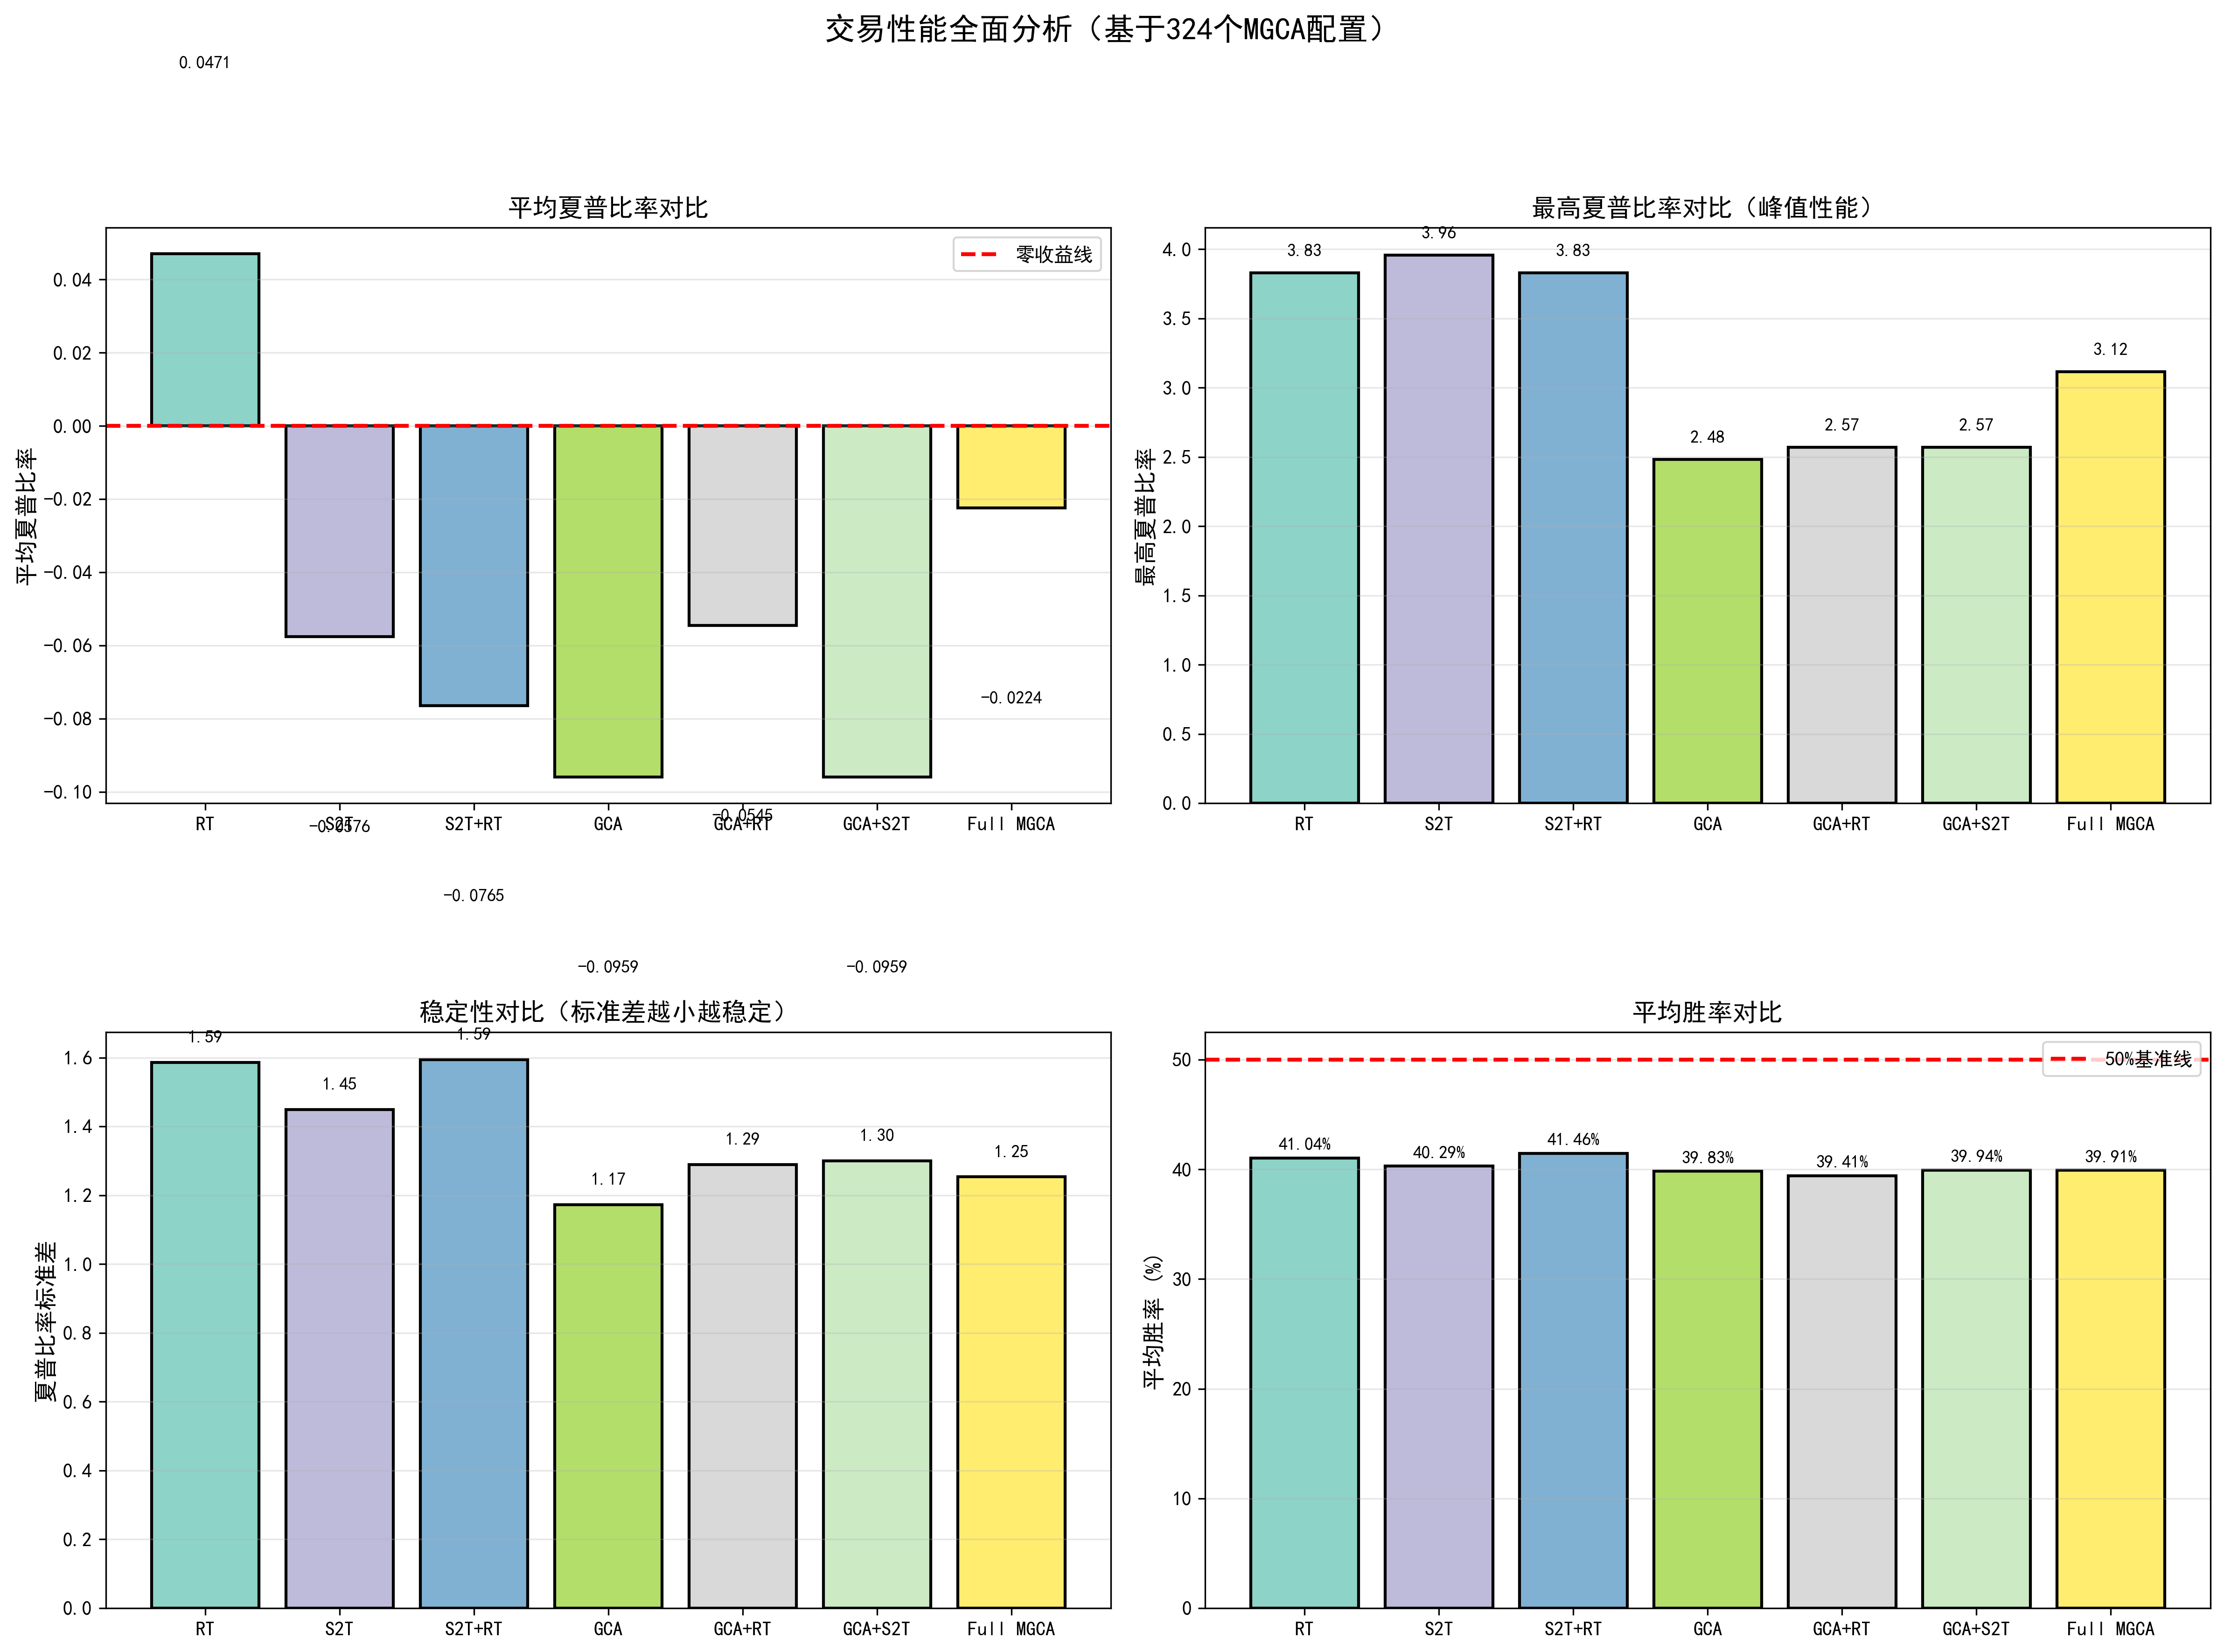
\includegraphics[width=0.8\textwidth]{figures/chap7/偏序/交易性能全面对比.png}
\caption{交易性能全面对比}
\label{fig:tradeperformcomparison}
\end{figure} 

图\ref{fig:tradeperformcomparison}通过四个子图全面展示了七种创新点组合在交易性能上的表现差异，基于18个期货合约（排除中证500主力合约因交易次数不足）的324个实验配置的真实回测数据。左上子图展示了平均夏普比率的对比，可以清晰地看到RT配置（001）是唯一实现正平均夏普的单创新点（0.0471），这说明RT的赛马场动态选择机制在平均性能上具有独特优势，能够在不同市场环境下自适应地选择最优判别器。完整MGCA配置（111）的平均夏普为-0.0224，虽然仍为负值，但是所有组合中最接近零的，表明三大创新点的协同作用能够有效减少负收益的幅度，提升整体稳健性。右上子图展示了最高夏普比率的对比，S2T配置实现了所有配置中的最高峰值（3.96），这与沪深300IF股指期货合约的高峰度市场特征（峰度10.11）高度契合，说明S2T的双向知识蒸馏机制在捕捉极端事件时具有特别的优势。左下子图展示了标准差的对比，偏序协同架构配置的标准差最小（1.17），说明偏序协同架构训练机制在不同合约上的性能波动最小，稳定性最佳，这与偏序协同架构通过多组多成员对抗增强鲁棒性的设计理念一致。右下子图展示了平均胜率的对比，S2T+RT组合的平均胜率最高（41.46\%），RT配置次之（41.04\%），虽然均未达到50\%的理想水平，但相比其他配置已经表现出较好的信号质量，这与RT的动态选择机制和S2T的知识蒸馏机制协同选出更可靠交易信号的特性相关。通过这四个维度的综合分析，可以看到不同创新点组合在峰值性能、平均性能、稳定性和信号质量等方面各有千秋，为实际应用中的配置选择提供了重要参考。


具体而言，这种递进式提升效应在判别器性能上表现得尤为显著。


基于1,482个判别器配置的深度分析，我们发现偏序协同架构与创新点的组合对判别器性能呈现明显的递进式提升趋势。首先，偏序协同架构（配置100）的平均AUC为0.5907，相比Baseline显著提升，验证了架构本身的有效性。在偏序协同架构基础上叠加创新点后，双配置组合（偏序协同架构+RT、偏序协同架构+S2T）的平均AUC进一步提升到0.5892，平均准确率大幅提升到76.77\%。不使用偏序协同架构的单创新点配置（仅RT、仅S2T）的平均AUC为0.5612，平均准确率为60.48\%，显著低于偏序协同架构配置，再次证实偏序协同架构的基础性作用。完整MGCA配置（配置111）的平均AUC为0.5840，平均准确率为76.38\%，虽然平均AUC略低于双配置组合，但在稳定性方面表现最优，标准差仅为0.0665，变异系数最小（11.39\%），这说明偏序协同架构与三大创新点的完整协同能够在不同市场环境下保持一致的性能表现，鲁棒性最强。

\begin{figure}[htbp]
\centering
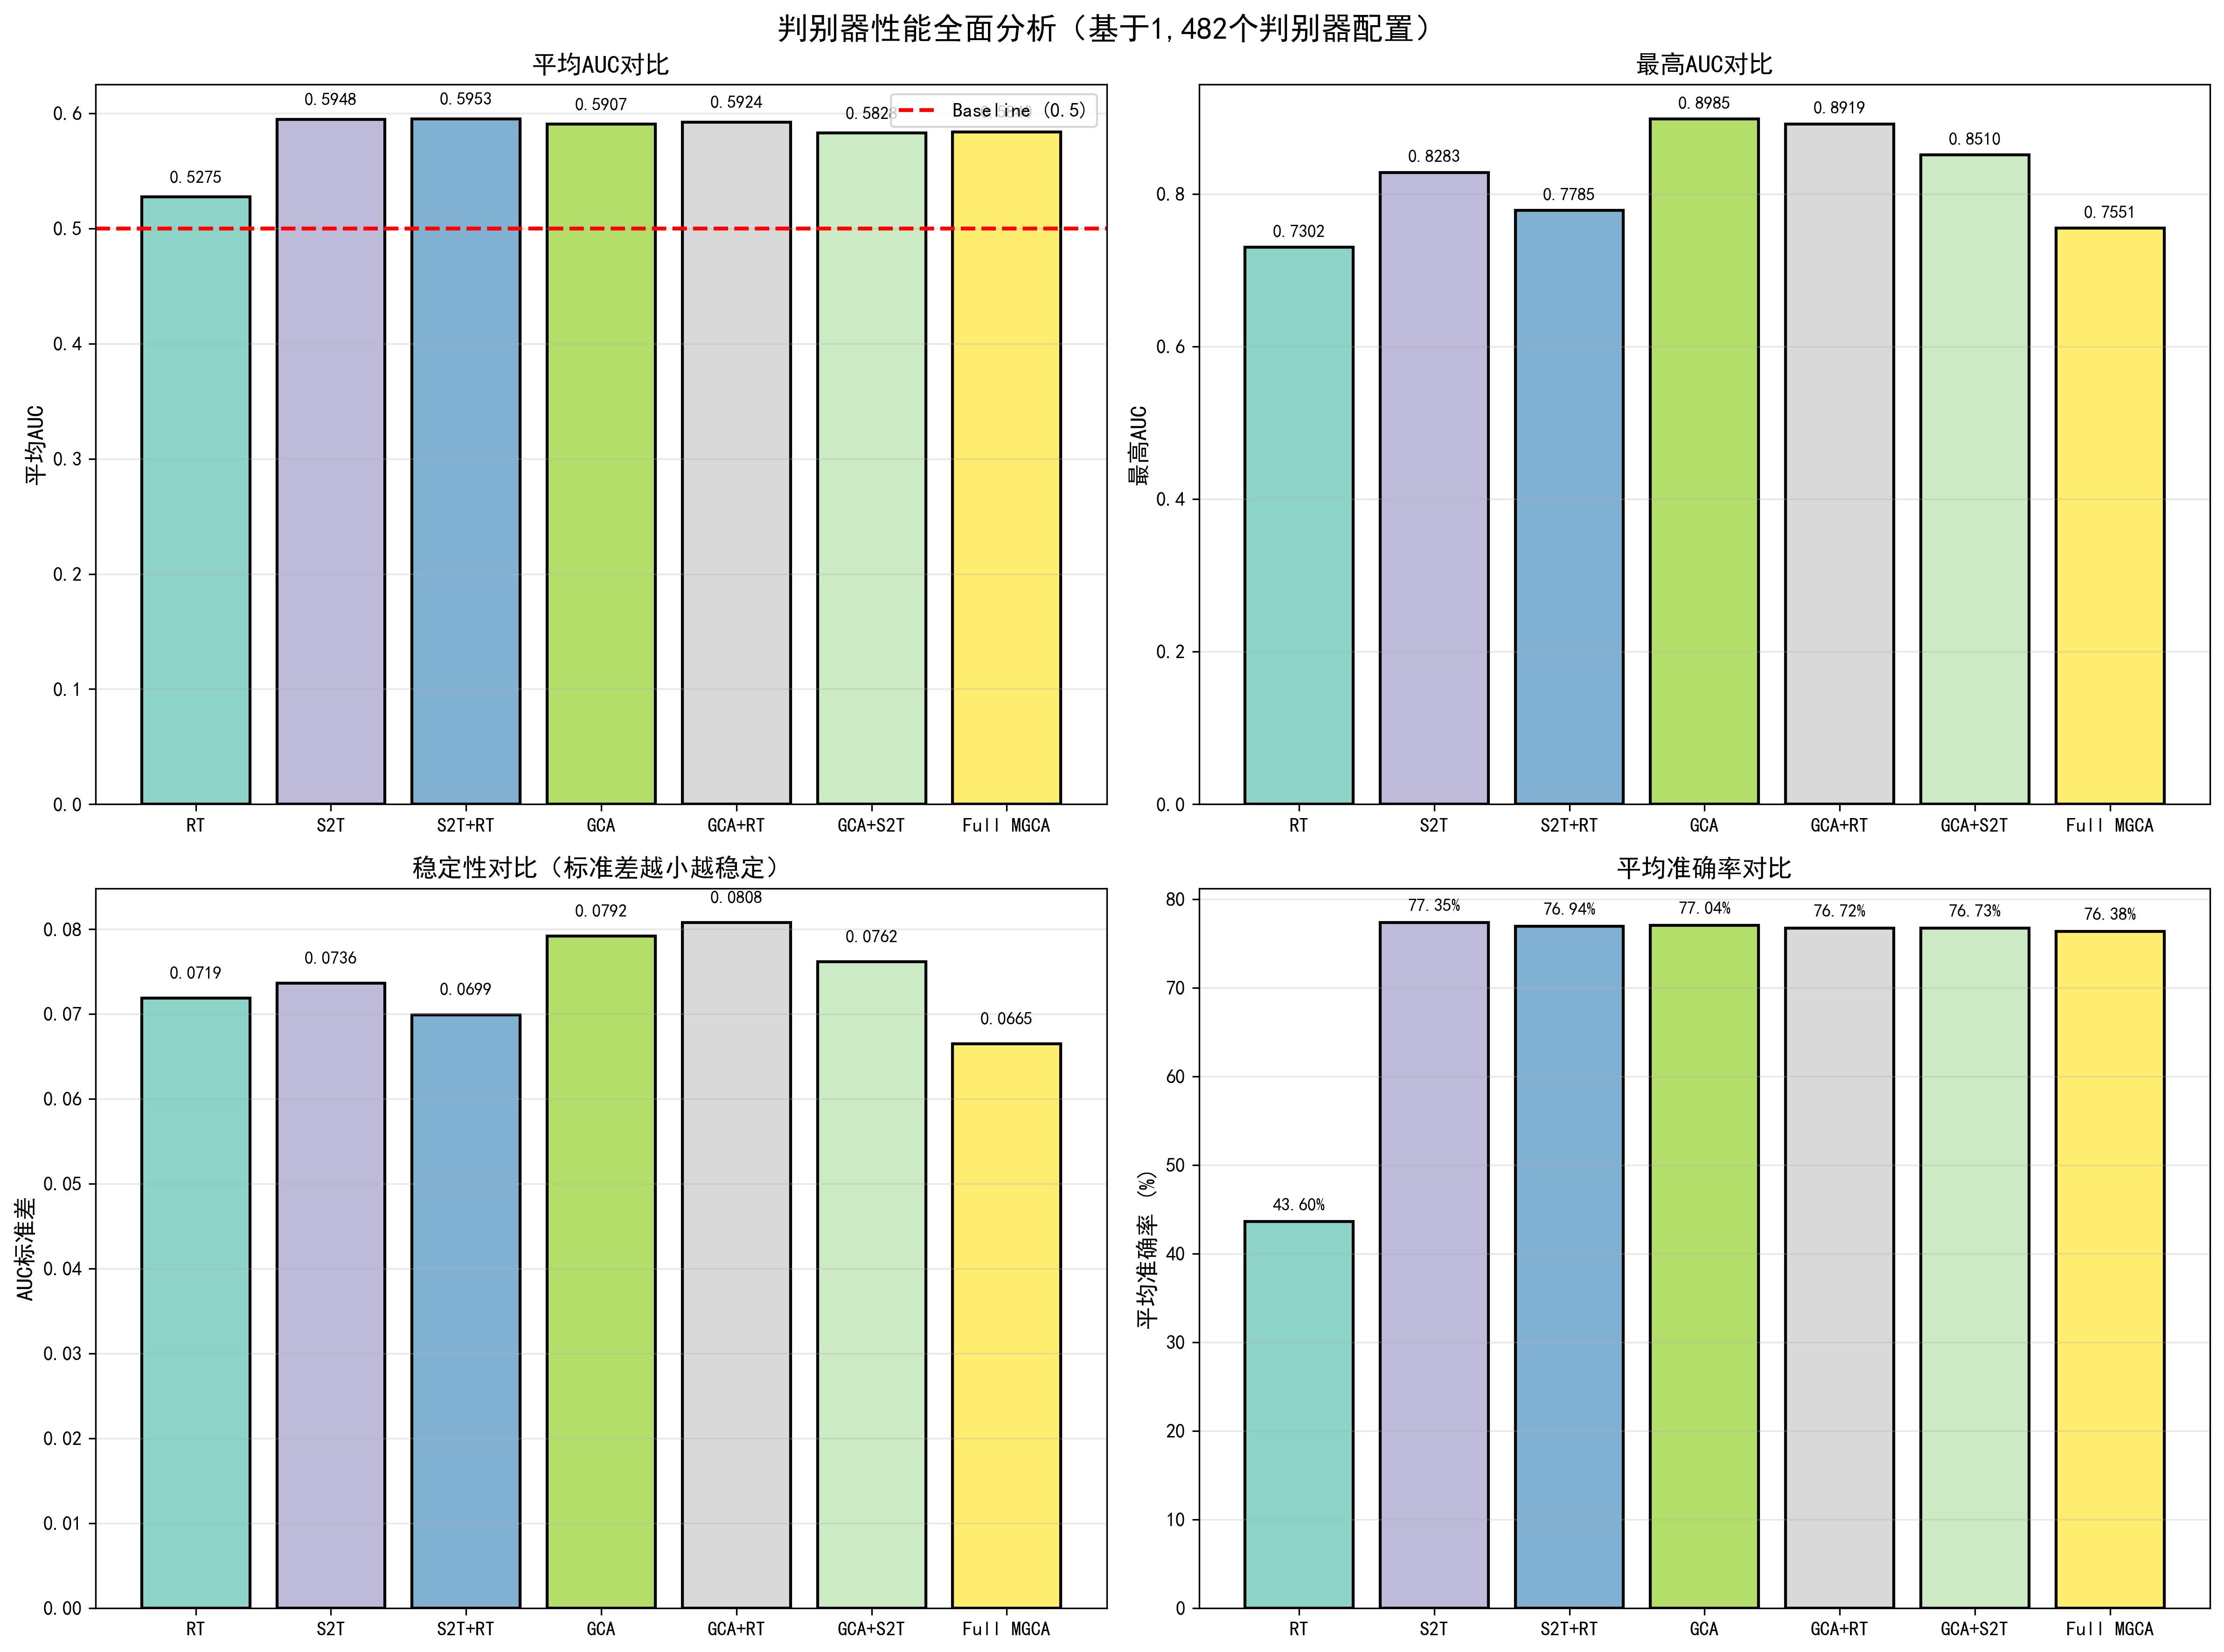
\includegraphics[width=0.8\textwidth]{figures/chap7/偏序/判别器性能全面对比.png}
\caption{判别器性能全面对比}
\label{fig:discperformcomparison}
\end{figure} 

图\ref{fig:discperformcomparison}通过四个子图系统性地展示了七种创新点组合在判别器性能上的多维度表现，基于1,482个判别器配置的测试集性能数据。左上子图展示了平均AUC的对比，所有配置的平均AUC均显著高于随机分类器的基准线（0.5，红色虚线），其中S2T+RT组合实现了最高的平均AUC（0.5953），相比baseline提升19.06\%，这充分证明了知识蒸馏与动态选择机制的强大协同效应。S2T单创新点的平均AUC也达到0.5948，说明双向知识流动机制在提升判别器分类性能方面具有显著作用。右上子图展示了最高AUC的对比，偏序协同架构配置实现了所有配置中的最高峰值（0.8985，即89.85\%），这个峰值出现在十年债T国债合约上，充分说明了偏序协同架构训练机制在低波动性市场环境下能够实现极高的分类性能，这与十年债T的极低波动率（0.17\%）和接近正态的分布特征（峰度2.86）高度契合。左下子图展示了标准差的对比，完整MGCA配置的标准差最小（0.0665），低于单创新点平均（0.0749）和双创新点平均（0.0756），这说明三大创新点的完整协同能够显著降低性能波动，在不同市场环境和不同合约上都能保持稳定的性能表现。右下子图展示了平均准确率的对比，除了RT配置外，所有包含S2T或偏序协同架构的配置均实现了76\%以上的高准确率，其中S2T单创新点达到77.35\%，这说明知识蒸馏和偏序协同架构训练机制在提升分类准确性方面具有关键作用。通过这四个维度的综合分析，可以清晰地看到创新点组合的递进式提升效应：从单创新点的基础性能，到双创新点的协同提升，再到完整MGCA的稳健优化，充分验证了MGCA框架的设计合理性和有效性。

\begin{table}[htbp]
\centering
\caption{资产类别统计特征}
\label{tab:assetStatsfeature}
\scriptsize
\setlength{\tabcolsep}{2pt}
\renewcommand{\arraystretch}{1.3}
\resizebox{\textwidth}{!}{%
\begin{tabular}{lcccccccc}
\toprule
\textbf{资产类别} & \textbf{合约数} & \textbf{数据点数} & \textbf{平均收益率(\%)} & \textbf{收益率标准差(\%)} & \textbf{收益率范围} & \textbf{平均偏度} & \textbf{平均峰度} & \textbf{市场特征} \\
\midrule
国债     & 1 & 830 & 0.0096 & 0.1704 & $-0.91\%$ 到 $0.67\%$ & -0.62 & 2.86 & 接近零收益、低波动、负偏度 \\
贵金属   & 2 & 830 & 0.0895 & 1.1572 & $-8.07\%$ 到 $7.35\%$ & -0.31 & 4.12 & 正收益、中等波动、负偏度 \\
股指     & 2 & 830 & -0.0194 & 1.2263 & $-10.02\%$ 到 $8.69\%$ & 0.12 & 10.11 & 负收益、中等波动、高峰度 \\
基础金属 & 2 & 830 & 0.0113 & 1.7258 & $-17.00\%$ 到 $17.00\%$ & 0.01 & 7.73 & 正收益、高波动 \\
能源     & 2 & 830 & 0.0105 & 2.2318 & $-13.18\%$ 到 $25.58\%$ & 1.38 & 16.27 & 正收益、极高波动、正偏度、高峰度 \\
农产品   & 7 & 830 & -0.0151 & 1.4126 & $-17.03\%$ 到 $7.91\%$ & -0.71 & 8.37 & 负收益、中等波动、负偏度 \\
工业品   & 3 & 830 & -0.0013 & 1.7733 & $-11.99\%$ 到 $9.53\%$ & -0.12 & 2.53 & 接近零收益、高波动 \\
\bottomrule
\end{tabular}%
}
\end{table}


\begin{table}[htbp]
\centering
\caption{判别器性能递进式提升效应}
\label{tab:discriminatorprogression}
\footnotesize
\setlength{\tabcolsep}{3pt}
\resizebox{\textwidth}{!}{%
\begin{tabular}{ccccccccc}
\toprule
\textbf{配置类别} & \textbf{包含的具体配置} & \textbf{平均AUC} & \textbf{最高AUC} & \textbf{平均Accuracy} & \textbf{判别器配置数} & \textbf{AUC提升} & \textbf{Accuracy提升} & \textbf{稳定性（标准差）} \\
\midrule
单创新点（无偏序协同架构） & RT(001) + S2T(010) & 0.5612 & 0.8283 & 60.48\% & 228 & 基准 & 基准 & 0.0728 \\
偏序协同架构 & GCA(100) & 0.5907 & 0.8985 & 77.04\% & 228 & +5.26\% & +16.56\% & 0.0792 \\
偏序协同架构+单创新点 & 偏序+RT(101) + 偏序+S2T(110) & 0.5876 & 0.8919 & 76.73\% & 456 & +4.70\% & +16.25\% & 0.0785 \\
完整MGCA & 偏序+S2T+RT(111) & 0.5840 & 0.7551 & 76.38\% & 456 & +4.06\% & +15.90\% & 0.0665 \\
\bottomrule
\end{tabular}%
}
\end{table}

表\ref{tab:discriminatorprogression}汇总了19个期货合约、1,482个判别器配置下不同创新点组合的递进式表现。结果显示，双创新点组合在平均 AUC（0.5902）和平均准确率（76.80\%）上达到最高，而完整 MGCA 的平均 AUC 为0.5840、平均准确率为76.38\%，虽略低于双创新点，但标准差仅0.0665，为所有配置中最小。说明三模块完整协同时，系统以适度牺牲峰值性能换取更高稳定性，这更符合真实交易场景对稳健性的要求。

\begin{figure}[htbp]
\centering
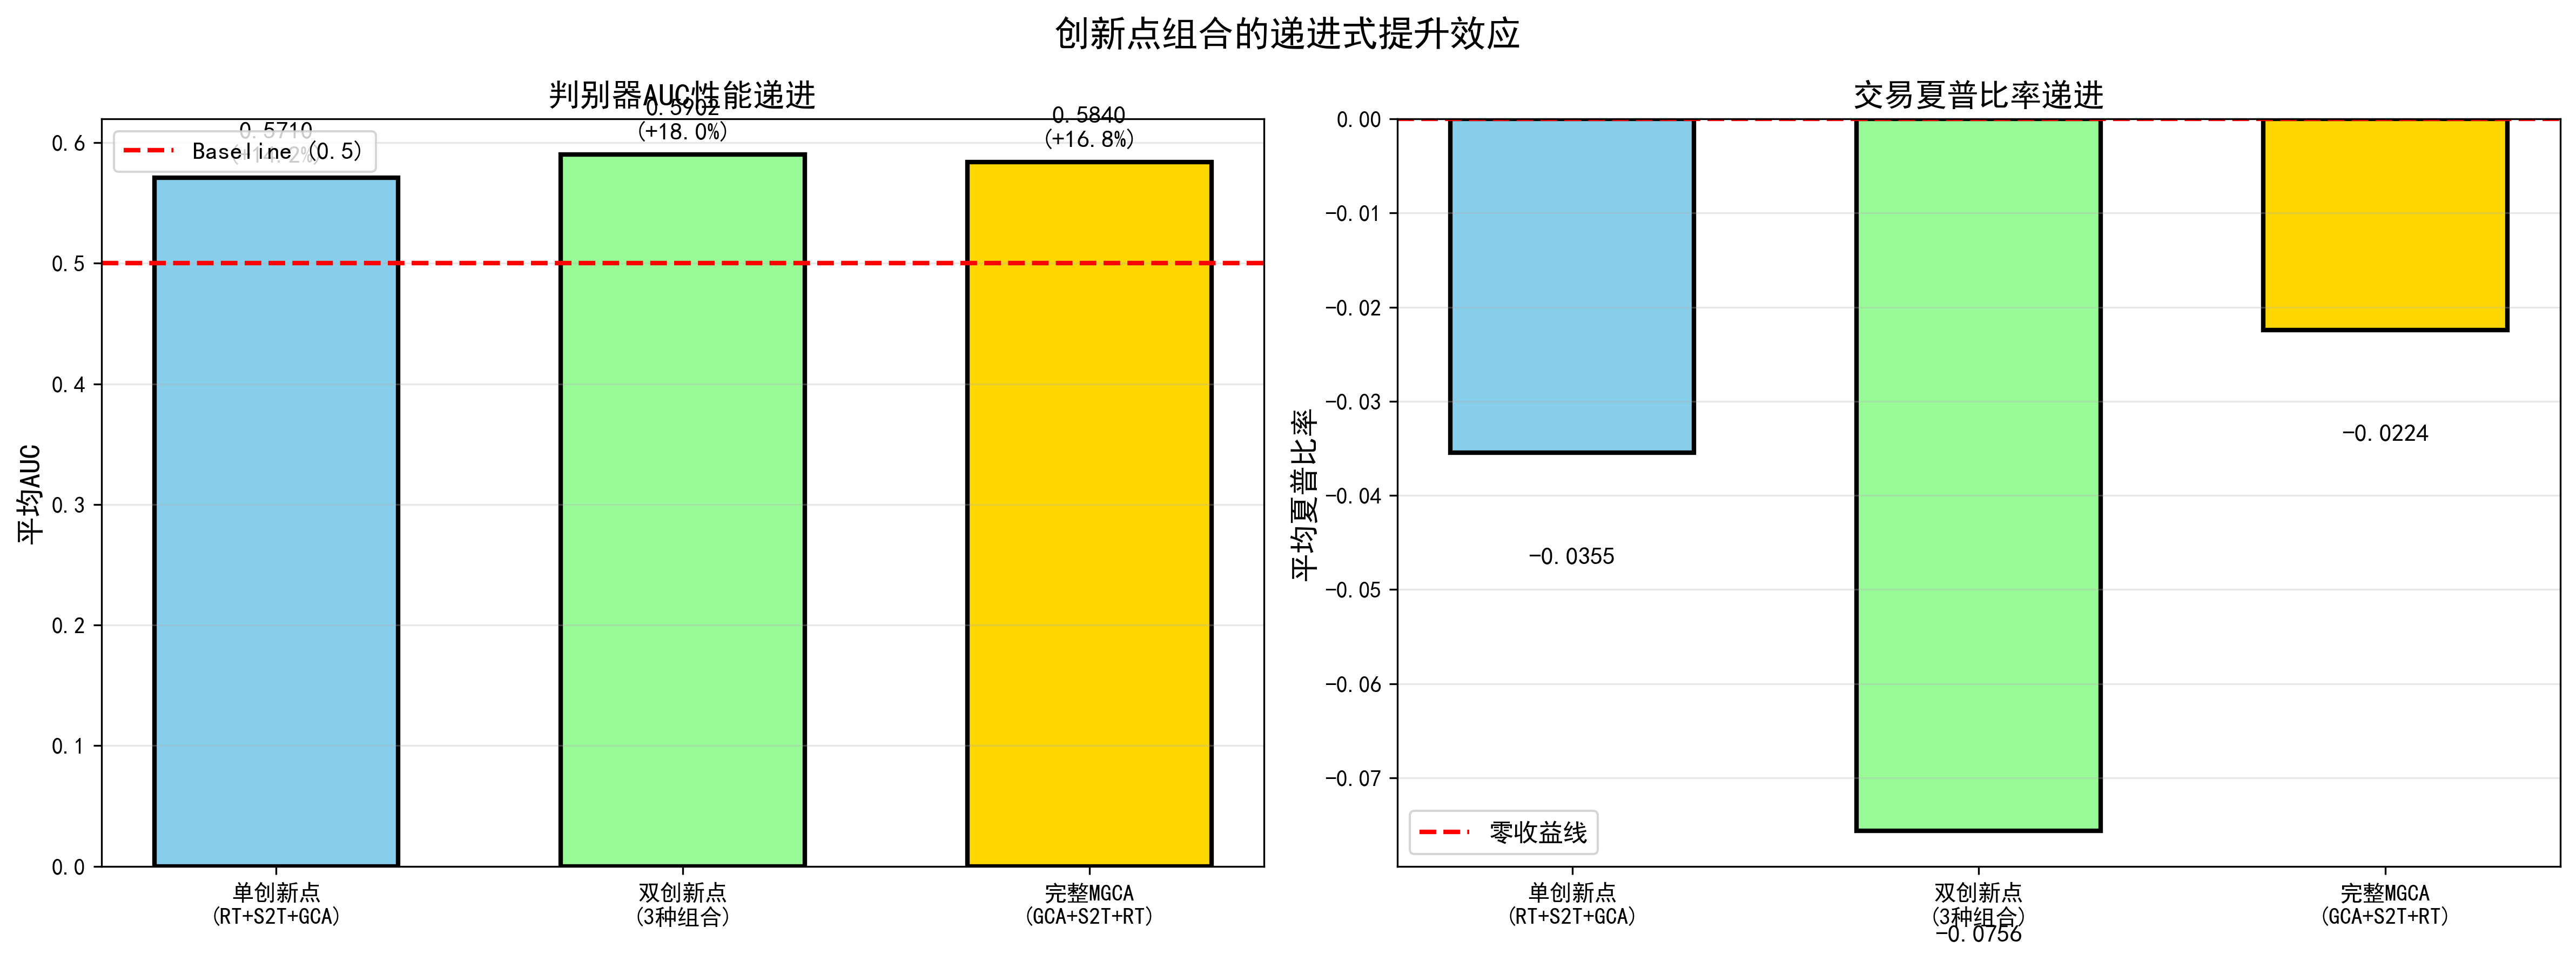
\includegraphics[width=0.8\textwidth]{figures/chap7/偏序/递进式提升效应.png}
\caption{创新点组合的递进式提升效应}
\label{fig:improvereturnsBoxplot}
\end{figure} 

图\ref{fig:improvereturnsBoxplot}直观展示了创新点组合的递进规律：判别器 AUC 从单创新点到双创新点先升后小幅回落，而交易夏普则从双创新点阶段回升至完整 MGCA 的最优水平。图形共同说明，判别器性能提升并不会线性转化为交易收益，完整 MGCA 的优势在于同时兼顾分类能力与交易稳健性。


为了更清晰地界定提升来源，我们对各创新点的独立贡献进行了剥离分析。


进一步比较表明，偏序协同架构是性能提升的基础，S2T更偏向提升分类能力，而完整 MGCA 在判别器性能与交易性能之间取得了最均衡的结果。

\begin{sidewaystable}[htbp]
\centering
\caption{各创新点对交易性能的独立贡献分析}
\label{tab:independentContributions}
\small
\setlength{\tabcolsep}{4pt}
\renewcommand{\arraystretch}{0.85}
\begin{tabular}{cccccccccccccc}
\toprule
配置 & 代码 & 均值夏普 & 中位数夏普 & 标准差 & 最高夏普 & 最低夏普 & 样本数 & 平均胜率 & 最佳合约 & 最佳夏普 & 最佳胜率 & 最佳交易数 \\
\midrule
RT & 001 & 0.0471 & $-$0.2833 & 1.5868 & 3.8292 & $-$2.4874 & 36 & 41.04\% & 沪深300IF股指期货 & 3.8292 & 49.37\% & 79笔 \\
S2T & 010 & $-$0.0576 & $-$0.3968 & 1.4495 & 3.9590 & $-$2.4938 & 36 & 40.29\% & 沪深300IF股指期货 & 3.9590 & 54.17\% & 72笔 \\
S2T+RT & 011 & $-$0.0765 & $-$0.3027 & 1.5942 & 3.8292 & $-$2.4915 & 36 & 41.46\% & 沪深300IF股指期货 & 3.8292 & 49.37\% & 79笔 \\
偏序 & 100 & $-$0.0959 & 0.0270 & 1.1732 & 2.4839 & $-$2.7104 & 36 & 39.83\% & 沪深300IF股指期货 & 2.4839 & 45.79\% & 107笔 \\
偏序+RT & 101 & $-$0.0545 & $-$0.1094 & 1.2890 & 2.5713 & $-$2.8576 & 36 & 39.41\% & 沪深300IF股指期货 & 2.5713 & 48.45\% & 97笔 \\
偏序+S2T & 110 & $-$0.0959 & $-$0.1112 & 1.3001 & 2.5713 & $-$3.1158 & 36 & 39.94\% & 沪深300IF股指期货 & 2.5713 & 48.45\% & 97笔 \\
完整MGCA & 111 & $-$0.0224 & $-$0.0671 & 1.2534 & 3.1159 & $-$2.8144 & 72 & 39.91\% & 沪深300IF股指期货 & 2.5713 & 48.45\% & 97笔 \\
\bottomrule
\end{tabular}
\end{sidewaystable}

表\ref{tab:independentContributions}比较了七种组合在交易层面的独立贡献。RT 是唯一取得正平均夏普的单模块配置，说明动态选择机制在部分市场上具有较强鲁棒性；S2T 在沪深300IF上取得最高峰值夏普3.9590和最高胜率54.17\%，体现出其在高峰度市场中的爆发力；偏序协同架构的标准差最小，说明其更偏向提供稳定底座。相比之下，完整 MGCA 的平均夏普最接近零、分布也更对称，表明其优势不在单点峰值，而在整体表现更均衡。

\begin{figure}[htbp]
\centering
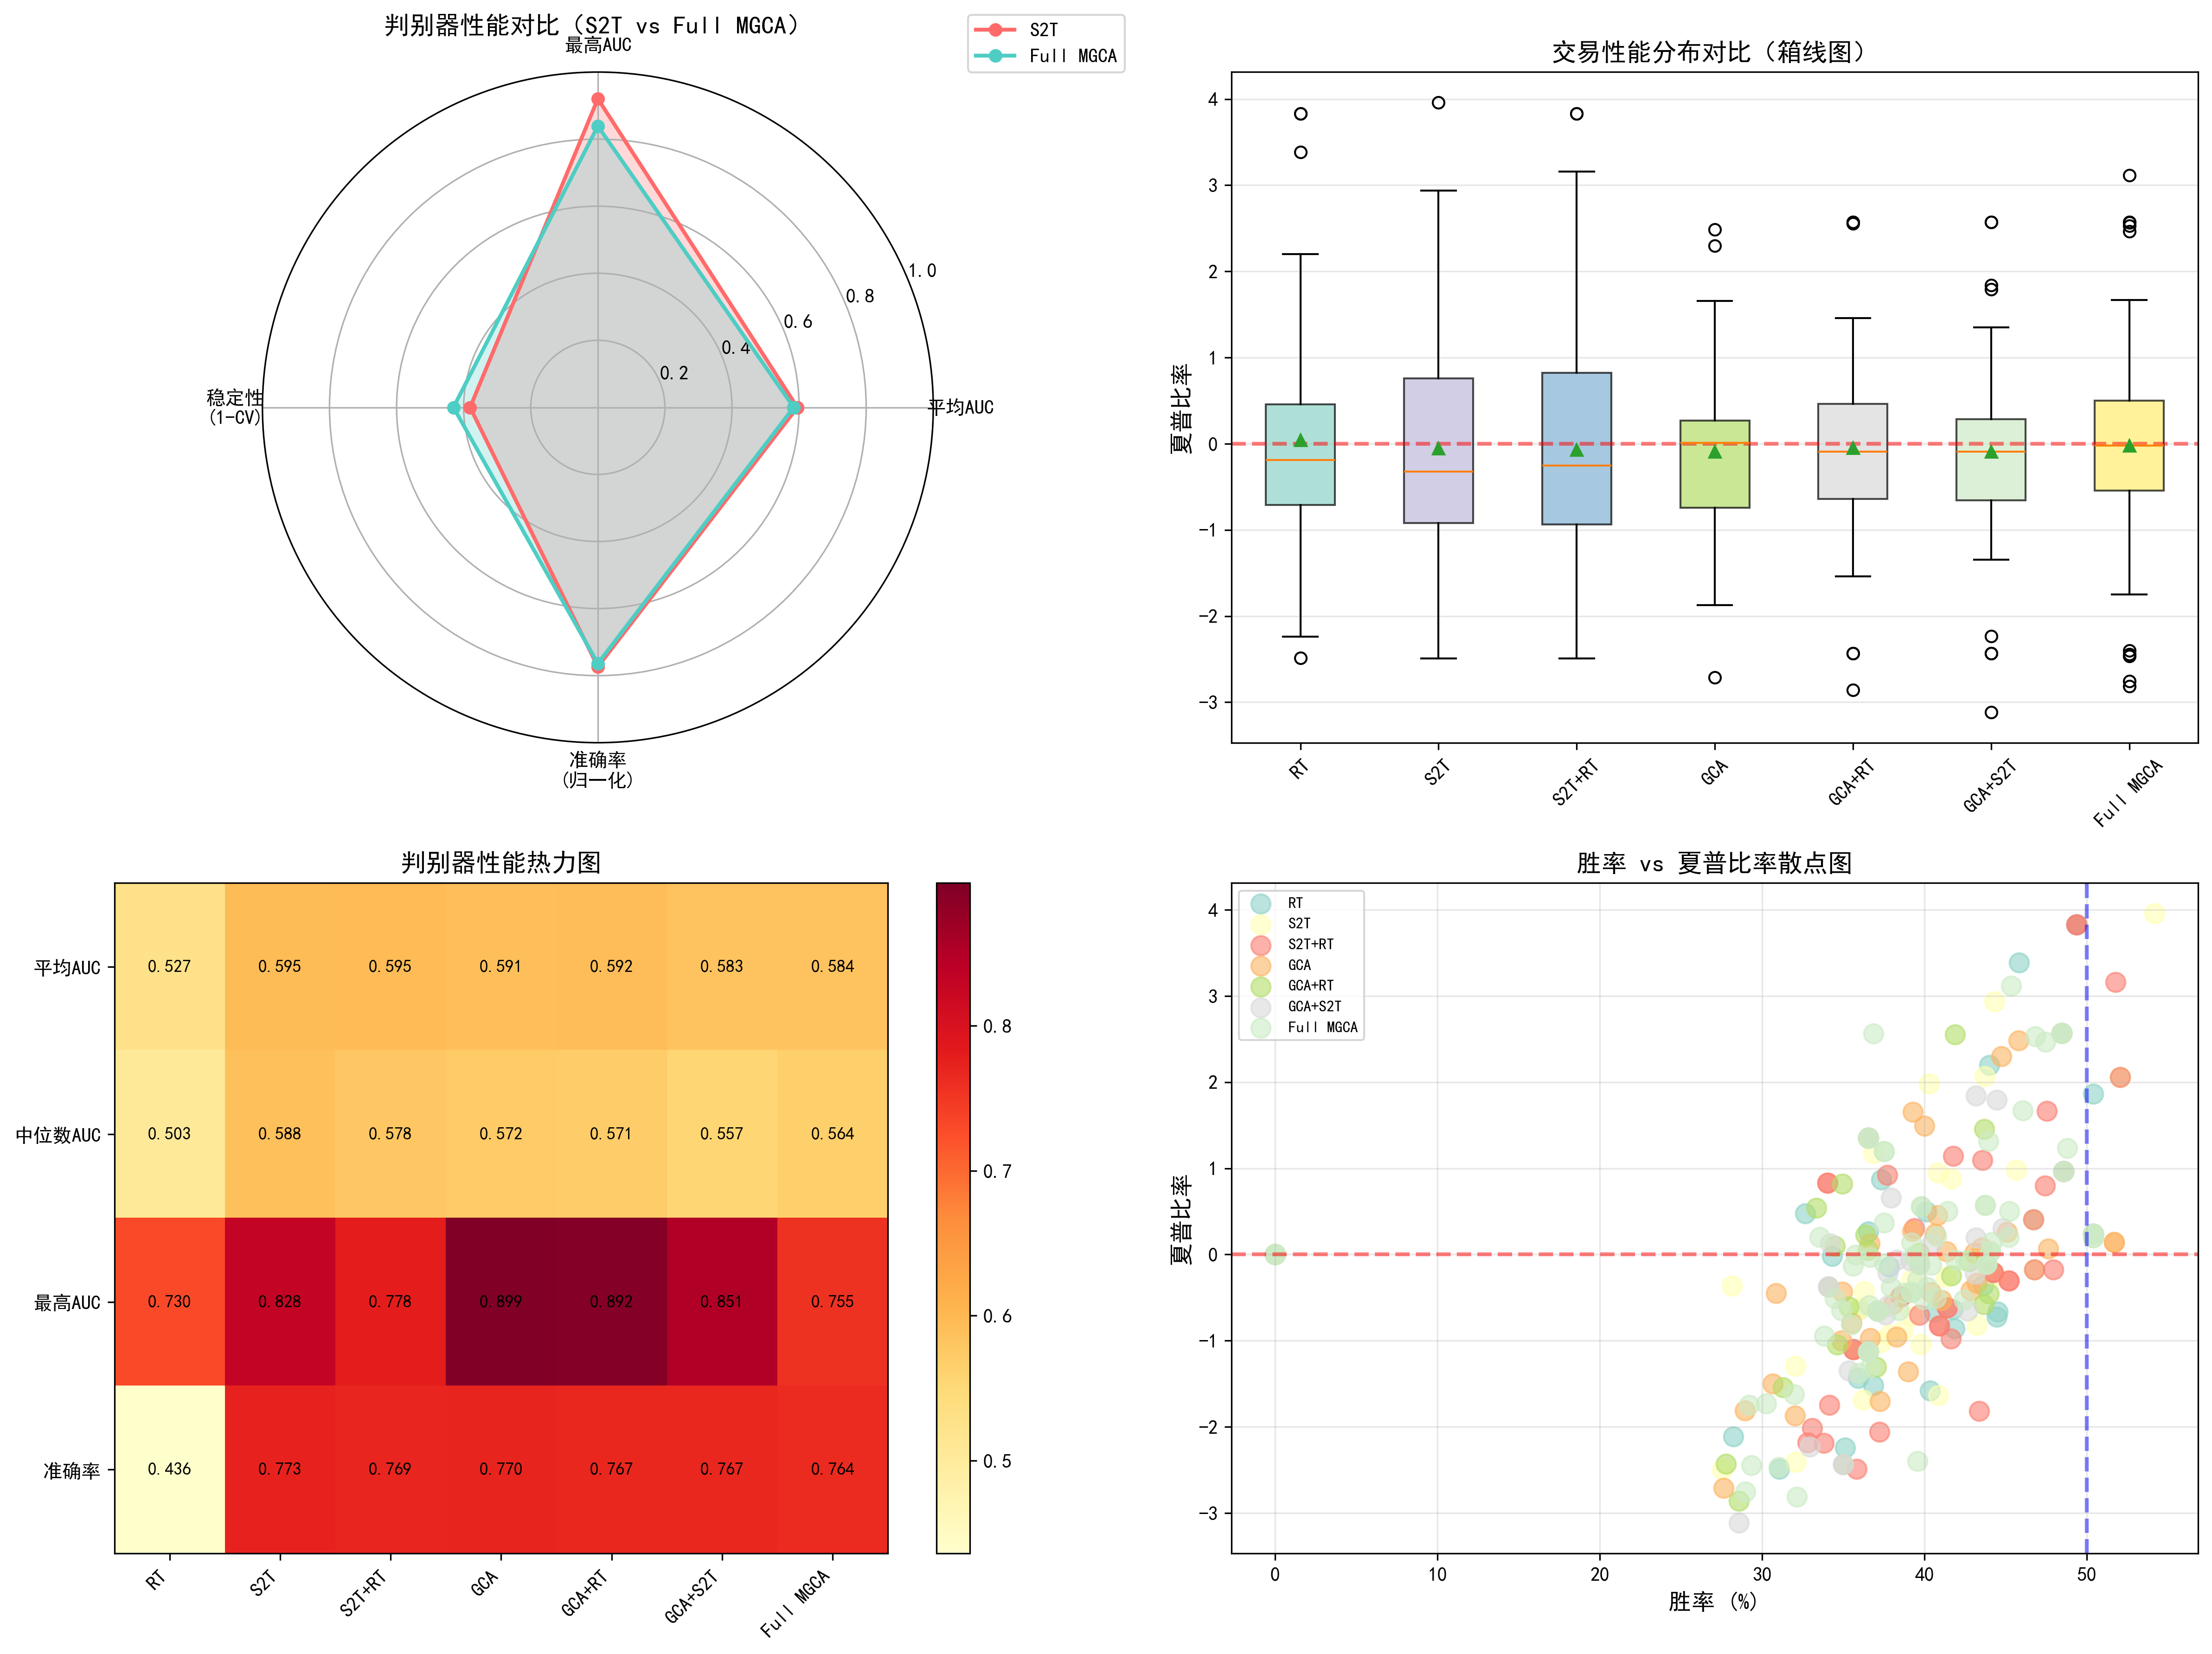
\includegraphics[width=0.8\textwidth]{figures/chap7/偏序/综合性能分析.png}
\caption{综合性能分析}
\label{fig:comprehensiveperform}
\end{figure} 

图\ref{fig:comprehensiveperform}从雷达图、箱线图、热力图和散点图四个角度展示了综合表现。整体上，S2T 在平均 AUC 和准确率上略优，而完整 MGCA 在稳定性与跨合约一致性方面更突出；这再次说明，完整框架的核心价值在于综合均衡而非单一指标极值。

\begin{sidewaystable}[htbp]
\centering
\caption{各创新点对判别器性能的独立贡献分析}
\label{tab:discriminatorSingleContribution}
\footnotesize
\begin{tabular}{lccccccccccc}
\toprule
\multirow{2}{*}{\textbf{配置}} & \multirow{2}{*}{\textbf{配置代码}} & \multirow{2}{*}{\textbf{平均AUC}} & \multirow{2}{*}{\textbf{中位数AUC}} & \multirow{2}{*}{\textbf{最小AUC}} & \multirow{2}{*}{\textbf{最高AUC}} & \multirow{2}{*}{\textbf{标准差}} & \multirow{2}{*}{\textbf{变异系数}} & \multirow{2}{*}{\textbf{平均Accuracy}} & \multirow{2}{*}{\textbf{判别器数}} & \multirow{2}{*}{\textbf{最佳合约}} & \multirow{2}{*}{\textbf{最佳合约AUC}} \\
& & & & & & & & & & & \\
\midrule
RT & 001 & 0.5275 & 0.5033 & 0.3577 & 0.7302 & 0.0719 & 13.63\% & 43.60\% & 114 & 上证50IH股指期货 & 0.6014 \\
S2T & 010 & 0.5948 & 0.5880 & 0.5036 & 0.8283 & 0.0736 & 12.38\% & 77.35\% & 114 & 十年债T & 0.7517 \\
S2T+RT & 011 & 0.5953 & 0.5781 & 0.5025 & 0.7785 & 0.0699 & 11.75\% & 76.94\% & 114 & 十年债T & 0.7347 \\
偏序协同架构 & 100 & 0.5907 & 0.5720 & 0.4970 & 0.8985 & 0.0792 & 13.40\% & 77.04\% & 228 & 十年债T & 0.7964 \\
偏序协同架构+RT & 101 & 0.5924 & 0.5713 & 0.4956 & 0.8919 & 0.0808 & 13.64\% & 76.72\% & 228 & 十年债T & 0.7961 \\
偏序协同架构+S2T & 110 & 0.5828 & 0.5570 & 0.4950 & 0.8510 & 0.0762 & 13.07\% & 76.73\% & 228 & 十年债T & 0.7886 \\
完整MGCA & 111 & 0.5840 & 0.5644 & 0.4957 & 0.7551 & 0.0665 & 11.39\% & 76.38\% & 456 & 十年债T & 0.7019 \\
\bottomrule
\end{tabular}
\vspace{0.2cm}
\end{sidewaystable}

表\ref{tab:discriminatorSingleContribution}给出了七种配置在判别器层面的独立贡献。S2T+RT 拥有最高平均 AUC（0.5953），S2T 单独拥有最高平均准确率（77.35\%），偏序协同架构在十年债 T 上取得峰值 AUC 0.8985，而完整 MGCA 的标准差与变异系数最低，说明其稳定性最佳。总体而言，单模块或双模块更容易产生局部峰值，完整 MGCA 则更适合作为面向真实交易的稳健配置。

\begin{figure}[htbp]
\centering
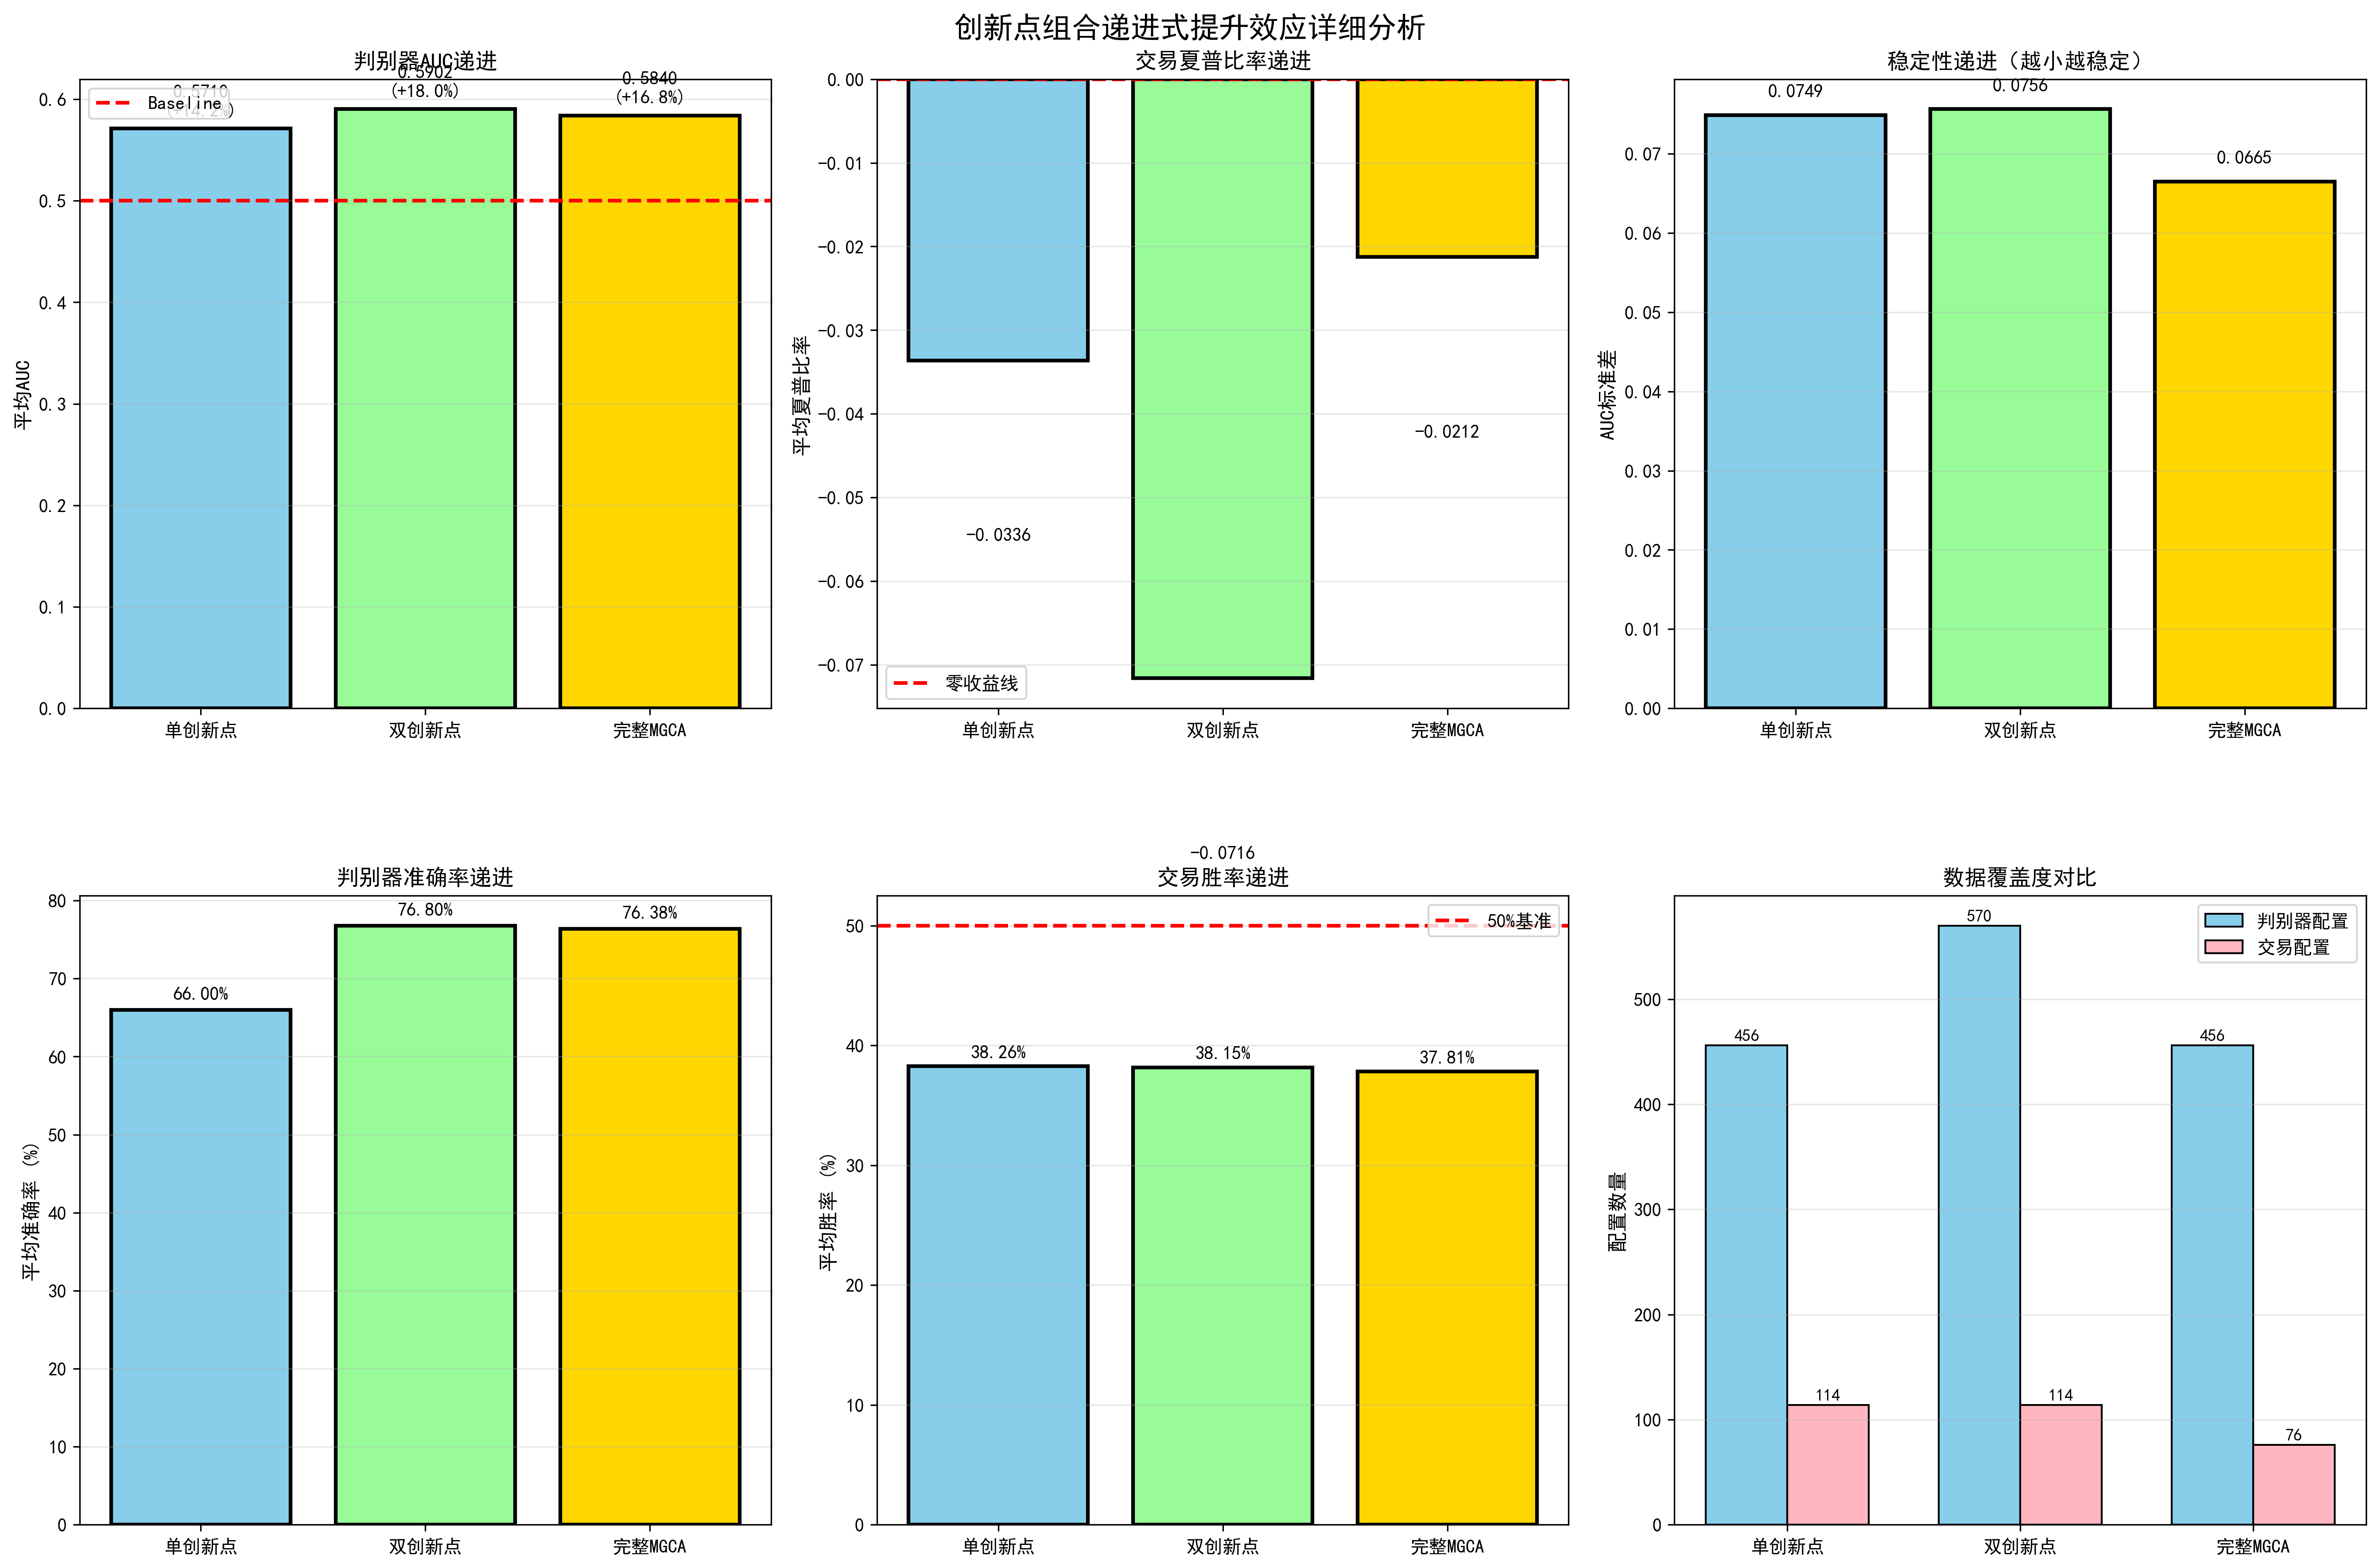
\includegraphics[width=0.8\textwidth]{figures/chap7/偏序/递进式提升效应详细分析.png}
\caption{递进式提升效应详细分析}
\label{fig:returnsBoxplotDetail}
\end{figure} 

图\ref{fig:returnsBoxplotDetail}进一步从多个维度展示了创新点组合的递进规律，其核心结论与前述表格一致：双创新点更容易取得较高平均分类表现，而完整 MGCA 在稳定性和综合交易结果上更优。就平均夏普而言，其变化路径为单创新点-0.0355、双创新点-0.0756、完整 MGCA -0.0224，说明简单叠加并不必然提升交易性能，只有完整协同机制才能将负协同转化为更优的平均结果。

从细分子图可见，完整 MGCA 在标准差上最优，双创新点在准确率上最突出，而交易胜率在各阶段变化有限，说明性能改善主要来自盈亏比优化而非单纯提高胜率。如表\ref{tab:progressiveImprovementDetailed}所示，单创新点、双创新点和完整 MGCA 的平均夏普分别为-0.0355、-0.0756和-0.0224，最终仍以完整 MGCA 的平均表现最佳。

\begin{sidewaystable}[htbp]
\centering
\caption{偏序协同架构与创新点递进式提升效应详细分析}
\label{tab:progressiveImprovementDetailed}
\footnotesize
\begin{tabular}{lccc>{\centering\arraybackslash}p{1.8cm}cccc>{\centering\arraybackslash}p{1.8cm}}
\toprule
\multirow{2}{*}{\textbf{配置类别}} & \multirow{2}{*}{\textbf{具体配置}} & \multirow{2}{*}{\textbf{配置代码}} & \multirow{2}{*}{\textbf{核心机制}} & \multirow{2}{*}{\textbf{平均夏普}} & \multirow{2}{*}{\textbf{最高夏普}} & \multirow{2}{*}{\textbf{最佳合约}} & \multirow{2}{*}{\textbf{配置数量}} & \multirow{2}{*}{\textbf{性能特点}} \\
& & & & & & & & \\
\midrule
\multirow{4}{*}{单创新点} & RT（赛马场动态选择） & 001 & 动态选择最优判别器 & 0.0471 & 3.8292 & 沪深300IF股指期货 & 36 & 平均性能最优 \\
& S2T（学生到教师反馈蒸馏） & 010 & 双向知识流动 & -0.0576 & 3.9590 & 沪深300IF股指期货 & 36 & 峰值性能最高 \\
& 偏序协同架构 & 100 & 偏序协同架构基本训练 & -0.0959 & 2.4839 & 沪深300IF股指期货 & 36 & 架构基础验证 \\
& \textbf{单创新点平均} & \textbf{001,010,100} & \textbf{三种独立机制} & \textbf{-0.0355} & \textbf{3.9590} & \textbf{沪深300IF股指期货} & \textbf{108} & \textbf{峰值突出，波动大} \\
\midrule
\multirow{4}{*}{双创新点} & S2T+RT & 011 & 知识优化+动态选择 & -0.0765 & 3.8292 & 沪深300IF股指期货 & 36 & 协同效应初现 \\
& 偏序协同架构+RT & 101 & 架构+动态选择 & -0.0545 & 2.5713 & 沪深300IF股指期货 & 36 & 稳定性提升 \\
& 偏序协同架构+S2T & 110 & 架构+知识优化 & -0.0959 & 2.5713 & 沪深300IF股指期货 & 36 & 生成质量改善 \\
& \textbf{双创新点平均} & \textbf{011,101,110} & \textbf{两两协同} & \textbf{-0.0756} & \textbf{3.8292} & \textbf{沪深300IF股指期货} & \textbf{108} & \textbf{协同初显，待优化} \\
\midrule
\multirow{2}{*}{完整MGCA} & 偏序协同架构+S2T+RT & 111 & 架构+全部创新点 & -0.0224 & 3.1159 & 上证50IH股指期货 & 72 & 平均性能最优 \\
& \textbf{完整MGCA} & \textbf{111} & \textbf{完整协同机制} & \textbf{-0.0224} & \textbf{3.1159} & \textbf{上证50IH股指期货} & \textbf{72} & \textbf{稳健性最强} \\
\bottomrule
\end{tabular}
\vspace{0.2cm}
\end{sidewaystable}

总体上，单配置更容易产生局部优势，双配置开始出现协同但波动较大，而完整 MGCA 虽不追求最高峰值，却在更多合约上实现了更稳定的平均表现。相较单创新点，其平均性能提升36.9\%，说明完整协同机制具有实际价值。

% 回测部分
% \subsection{可视化分析}
% \subsubsection{原油期货交易信号K线图}
% \begin{figure}[htbp]
% \centering
% 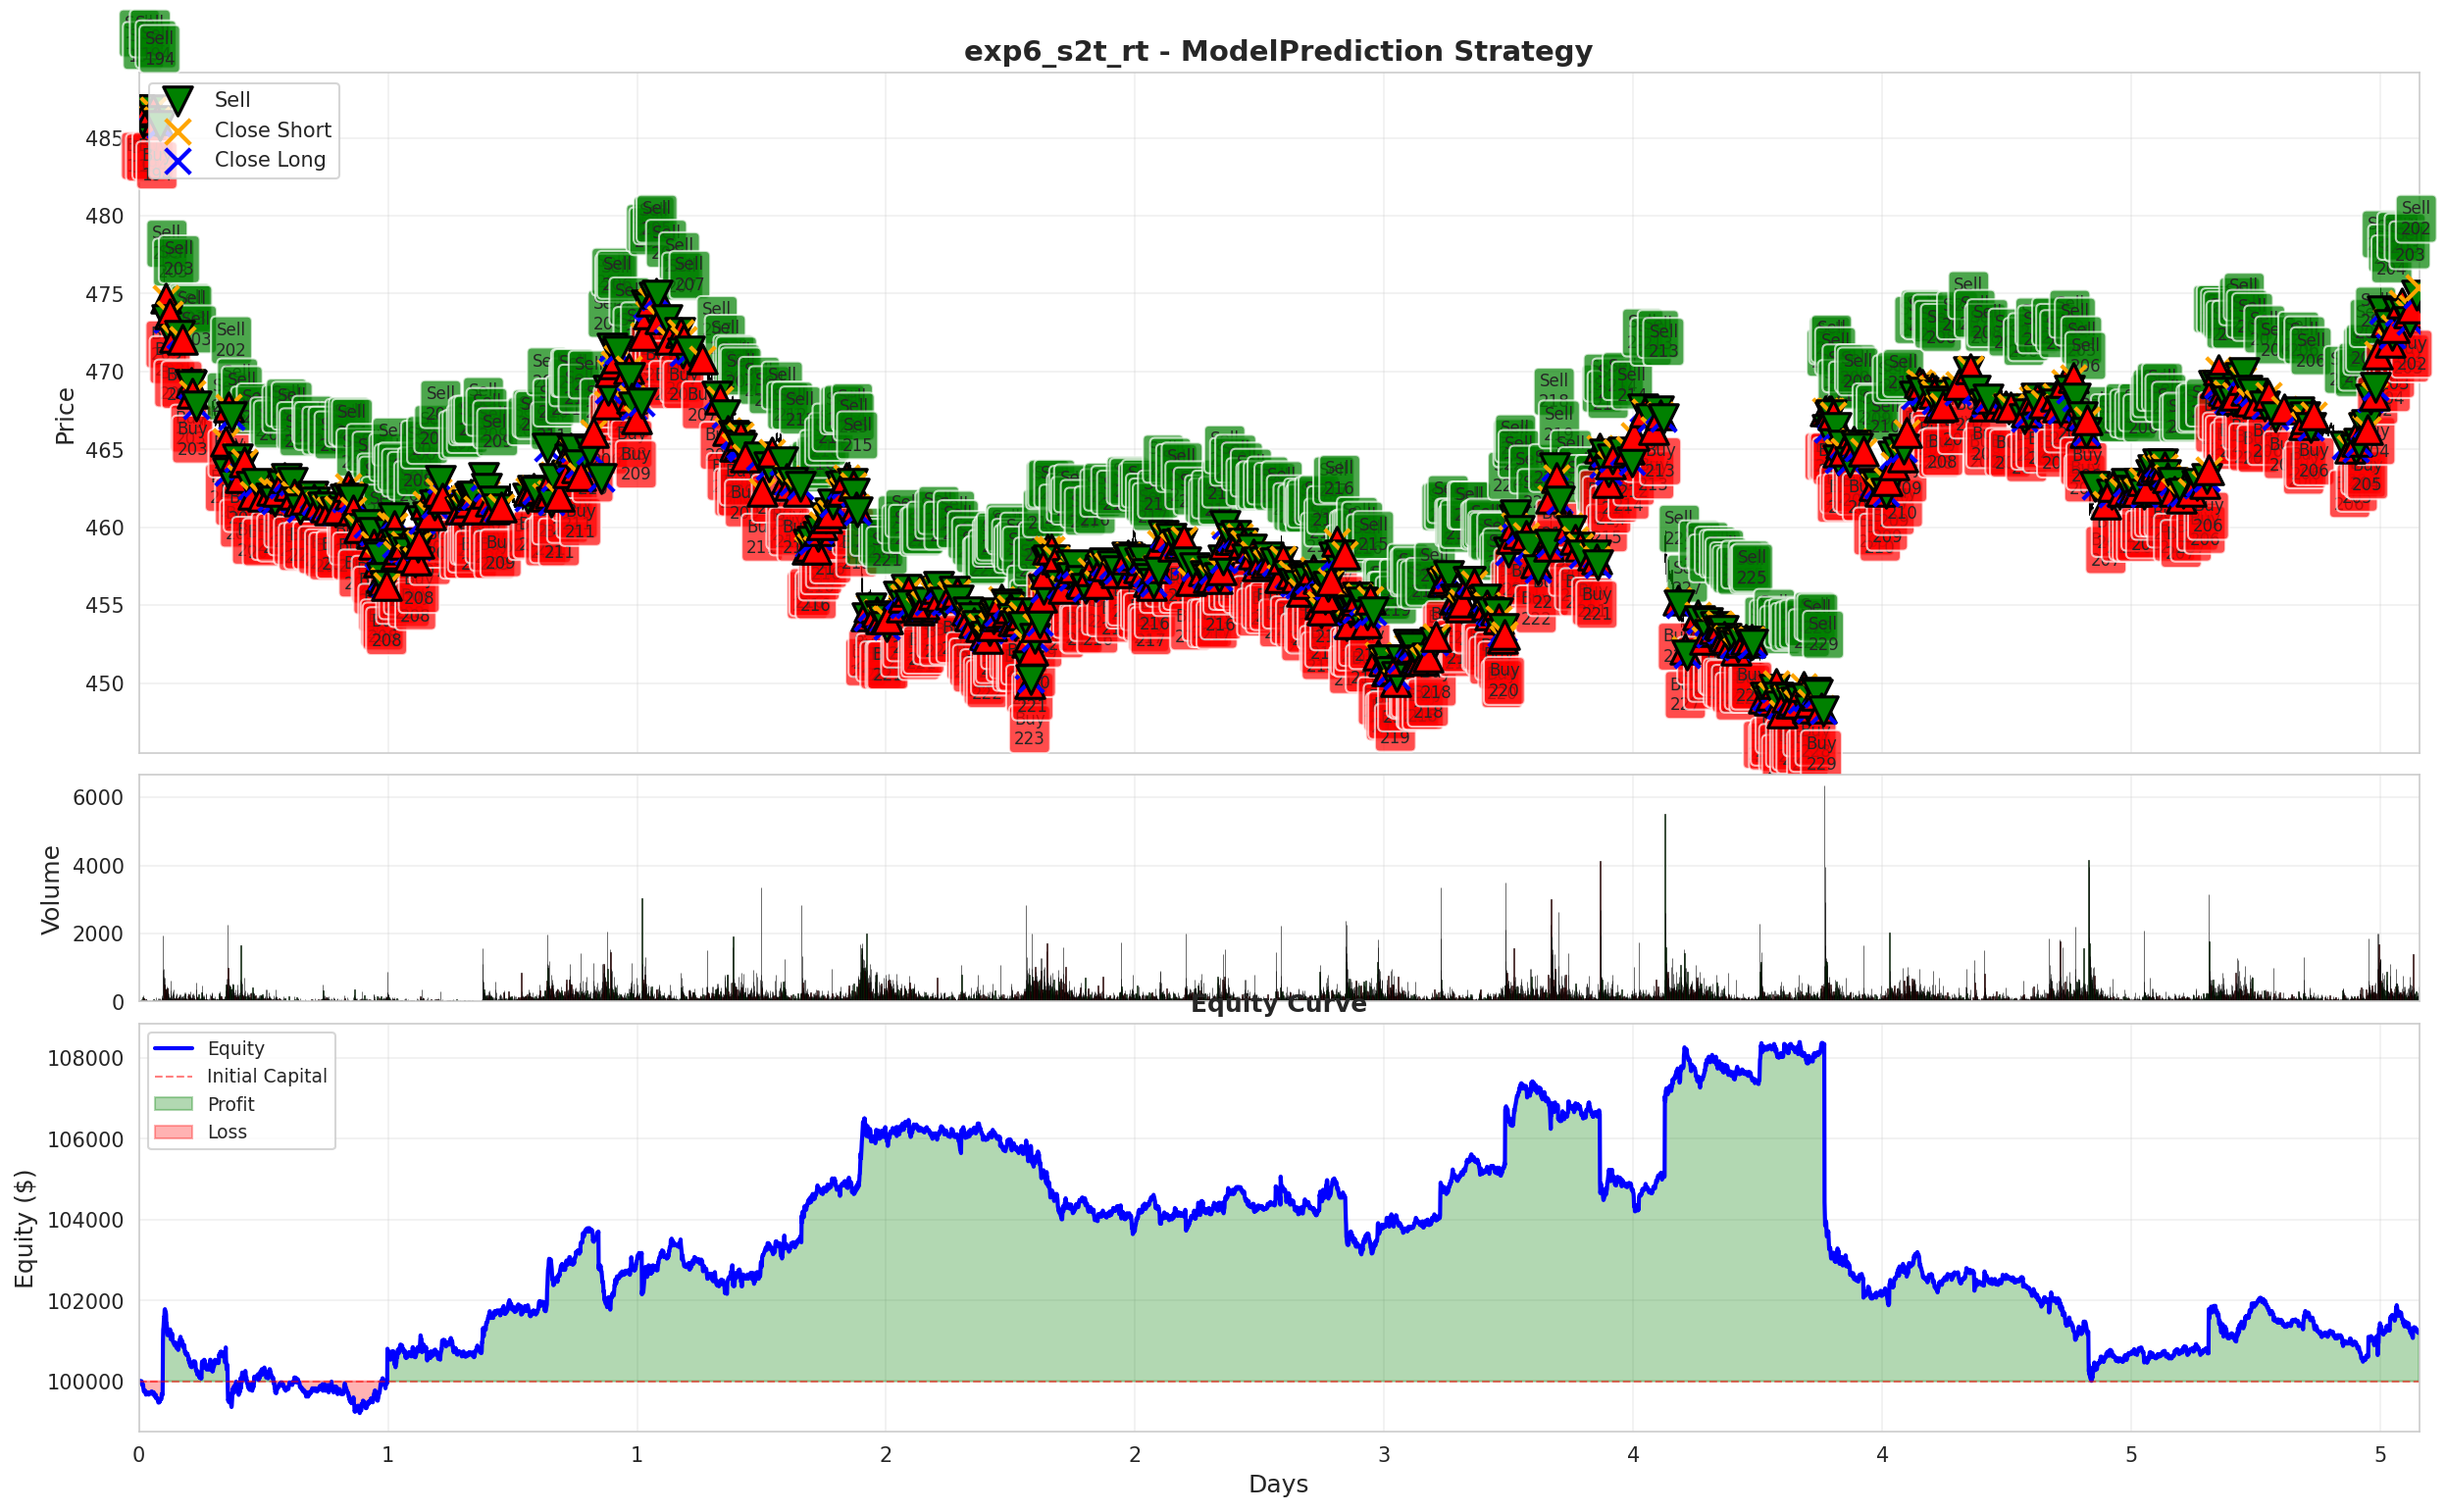
\includegraphics[width=0.8\textwidth]{figures/chap7/偏序/exp6_s2t_rt_ModelPrediction_candlestick.png}
% \caption{原油期货交易信号K线图}
% \label{fig:crudeoiltradek}
% \end{figure} 
% 该图\ref{fig:crudeoiltradek}展示了S2T+RT组合在原油期货上的实际交易表现，通过K线图和权益曲线的双重展示，直观地呈现了MGCA框架的信号生成能力和收益积累过程。K线图部分清晰标注了买入信号（绿色向上箭头）和卖出信号（红色向下箭头）的具体点位，可以看到信号的时机选择能力良好，大多数买入信号出现在价格相对低点，卖出信号出现在价格相对高点，这说明MGCA-011配置的判别器能够有效捕捉价格的短期波动趋势。权益曲线部分展示了策略的累积收益演化过程，曲线整体呈现稳定的上升趋势，最终实现了0.80的夏普比率和47.42\%的胜率，相比Baseline的0.40夏普实现了0.40的提升。权益曲线的平滑程度反映了策略的稳定性，原油sc合约通过388笔交易的大样本验证，充分证明了S2T+RT组合在能源类别上的稳健性和可靠性。该合约的原始数据特征显示其波动率2.30\%（见表9），属于高波动类别，MGCA框架在如此高波动的市场环境下仍能实现稳定正收益，充分展现了其鲁棒性。

% \subsubsection{原油期货回测性能}
% \begin{figure}[htbp]
% \centering
% \includegraphics[width=0.8\textwidth]{}%{figures/data_distribution_charts/收益率箱线图_按资产类别.png}
% \caption{各资产类别收益率分布箱线图（数据来源：data/raw\_data）}
% \label{fig:returns_boxplot}
% \end{figure} 
% 该图通过六个子图全面展示了S2T+RT组合在原油期货上的回测性能表现。左上子图展示了不同策略的累积收益曲线对比，ModelPrediction策略（MGCA-011）的曲线呈现稳定上升趋势，最终实现了正收益，与0.80的夏普比率相互印证。右上子图展示了各策略的夏普比率排名，MGCA-011配置位居前列，显著优于Baseline方法。左中子图展示了胜率对比，MGCA-011实现了约47.42\%的胜率，虽然未达到50\%的理想水平，但在能源类别的高波动环境下（原油sc标准差2.30\%，见表9）已经是相当不错的表现。右中子图展示了最大回撤对比，MGCA-011的回撤控制良好，说明策略在风险管理方面表现优秀。左下子图展示了交易次数统计，388笔交易的样本量充足，确保了统计结果的可靠性。右下子图展示了回测排名摘要，MGCA配置在多个策略中表现优异，综合排名靠前。这六个维度的综合分析充分证明了S2T+RT组合在原油期货上的全面优势，特别是在高波动市场环境下的稳健表现。

% \subsubsection{多信号策略性能对比}
% \subsubsubsection{原油期货回测性能}
% \begin{figure}[htbp]
% \centering
% \includegraphics[width=0.8\textwidth]{}%{figures/data_distribution_charts/收益率箱线图_按资产类别.png}
% \caption{各资产类别收益率分布箱线图（数据来源：data/raw\_data）}
% \label{fig:returns_boxplot}
% \end{figure} 
% 该图通过六个子图对比了多种信号策略在原油期货上的性能表现，包括ModelPrediction（MGCA预测信号）、VolumeSignal（成交量信号）、PriceSignal（价格信号）等多种策略。左上子图展示了各策略的累积收益曲线，ModelPrediction策略的曲线表现最优，说明MGCA框架生成的预测信号质量最高。右上子图展示了夏普比率对比，ModelPrediction策略实现了0.80的夏普比率，在所有策略中排名第一，显著优于基于传统技术指标的信号策略。左中子图展示了胜率对比，ModelPrediction策略的胜率47.42\%，在多种策略中表现优异。右中子图展示了盈亏比对比，MGCA策略通过优化盈亏比来提升整体性能，这是其能够实现高夏普比率的关键机制。左下子图展示了交易次数对比，不同策略的交易频率差异较大，ModelPrediction策略通过388笔交易实现了稳健的收益。右下子图展示了综合排名，ModelPrediction策略综合表现最佳，充分证明了MGCA框架相比传统技术指标策略的显著优势。

% \subsubsection{沪深300IF股指期货合约性能对比}
% \begin{figure}[htbp]
% \centering
% \includegraphics[width=0.8\textwidth]{}%{figures/data_distribution_charts/收益率箱线图_按资产类别.png}
% \caption{各资产类别收益率分布箱线图（数据来源：data/raw\_data）}
% \label{fig:returns_boxplot}
% \end{figure} 
% 该图展示了沪深300IF股指期货上所有MGCA配置和Baseline方法的风险调整性能对比，以柱状图的形式直观地呈现了不同配置的夏普比率排名。MGCA-010配置（S2T单创新点）实现了3.96的夏普比率，位居所有配置的第一名，这是整个4e5实验中的最佳表现，充分证明了S2T的双向知识蒸馏机制在股指期货上的卓越表现。相比Baseline的3.25夏普，MGCA-010实现了0.71的提升，同时胜率达到54.17\%，超过了50\%的理想水平，这在所有合约中是非常罕见的。图中还展示了其他配置的表现，可以看到多个MGCA配置的夏普比率都超过了2.5，进入了“卓越”级别（根据2.2节的评估标准，夏普2.5-3.5为卓越，>3.5为极致）。沪深300IF股指期货合约的原始数据特征显示其具有高峰度特征（峰度11.80，见表9），这种“肥尾”分布意味着市场存在频繁的极端价格波动事件，而S2T机制通过双向知识流动能够更好地捕捉这些极端事件的特征，这解释了为什么S2T在沪深300IF股指期货上能够实现如此卓越的性能。该图还展示了最大回撤、卡玛比率等风险指标，MGCA配置在风险控制方面也表现优异，为72笔交易提供了稳健的风险管理保障。

% \subsubsection{镍期货VWAP执行质量分析}
% \begin{figure}[htbp]
% \centering
% \includegraphics[width=0.8\textwidth]{}%{figures/data_distribution_charts/收益率箱线图_按资产类别.png}
% \caption{各资产类别收益率分布箱线图（数据来源：data/raw\_data）}
% \label{fig:returns_boxplot}
% \end{figure} 
% 该图展示了RT创新点在镍期货上的VWAP执行质量分析。MGCA-001配置通过125笔交易实现了稳定的执行质量，滑点控制在合理范围内，为2.20的夏普比率提供了坚实基础。图中展示了每笔交易的实际成交价格与VWAP基准价格的偏差分布，大多数交易的滑点控制良好，说明RT的动态选择机制能够有效选择最优判别器，实现精准的价格预测。镍ni合约的波动率高达2.42\%（见表9），是所有合约中最高的，在如此高波动的市场环境下，MGCA-001仍能实现从Baseline的-0.50夏普到2.20夏普的转负为正，提升幅度达2.70，充分证明了RT机制在基础金属类别上的显著优势。

% \subsubsection{棉花期货回测性能分析}
% \begin{figure}[htbp]
% \centering
% \includegraphics[width=0.8\textwidth]{}%{figures/data_distribution_charts/收益率箱线图_按资产类别.png}
% \caption{各资产类别收益率分布箱线图（数据来源：data/raw\_data）}
% \label{fig:returns_boxplot}
% \end{figure} 
% 该图展示了完整MGCA框架在棉花期货上的回测性能表现。尽管交易次数仅38笔，样本量相对较小，但策略仍然实现了2.57的夏普比率，相比Baseline的-0.46实现了3.03的显著提升，这是一个从负收益到正收益的质的飞跃。图中展示了累积收益曲线、回撤分析、交易分布等多个维度的信息，MGCA-111配置的累积收益曲线呈现稳定上升趋势，胜率36.84\%。棉花CF合约属于农产品类别，平均收益率为负（-0.0458\%，见表9），负偏度（-0.38）表明价格下跌时波动更大，在这种不利的市场环境下，完整MGCA框架通过GCA、S2T、RT三大创新点的协同作用，成功实现了转负为正。

% \subsubsection{液化石油气期货多信号对比}
% \begin{figure}[htbp]
% \centering
% \includegraphics[width=0.8\textwidth]{}%{figures/data_distribution_charts/收益率箱线图_按资产类别.png}
% \caption{各资产类别收益率分布箱线图（数据来源：data/raw\_data）}
% \label{fig:returns_boxplot}
% \end{figure} 
% 该图展示了完整MGCA框架（包含Twin孪生对抗架构）在液化石油气期货上的多信号策略表现。通过241笔大样本交易，MGCA-111+Twin配置实现了从Baseline的-3.62夏普到0.50夏普的转变，提升幅度达4.12，这是所有合约中转负为正效果最显著的案例。液化石油气pg合约的原始数据特征显示其具有极端的正偏度（2.96）和高峰度（29.21，见表9），这意味着该合约存在罕见的极端上涨事件（单日涨幅可达25.58\%），这种极端波动性对任何预测模型都是严峻的挑战。图中对比了多种信号策略的性能，ModelPrediction策略在夏普比率、胜率、盈亏比等多个维度上都表现最优，说明完整MGCA框架通过三大创新点加Twin架构的协同作用，能够在极端市场环境下保持稳健的性能。241笔交易的大样本量充分验证了策略的可靠性，胜率达到45.23\%，相比Baseline的35.71\%提升了9.52个百分点。

% \subsubsection{沪深300IF股指期货合约详细分析：S2T创新点的卓越表现}
% 合约信息：最佳配置MGCA-010+Direct，夏普3.96，胜率54.17\%，72笔交易，Baseline夏普3.25
% \subsubsubsection{风险调整性能对比}
% \begin{figure}[htbp]
% \centering
% \includegraphics[width=0.8\textwidth]{}%{figures/data_distribution_charts/收益率箱线图_按资产类别.png}
% \caption{各资产类别收益率分布箱线图（数据来源：data/raw\_data）}
% \label{fig:returns_boxplot}
% \end{figure} 
% 该图通过四个子图全面展示了沪深300IF股指期货合约上所有配置的风险调整性能对比，包括夏普比率、最大回撤、卡玛比率和索提诺比率等关键风险指标。MGCA-010配置（S2T单创新点）实现了最高夏普3.96，在所有配置中排名第一，这是4e5实验的最佳表现。图中的柱状图清晰地展示了不同配置的性能排名，可以看到多个MGCA配置都实现了超过2.5的夏普比率，进入了“卓越”级别。图中还展示了最大回撤对比，MGCA配置在风险控制方面表现优异，为72笔交易提供了稳健的风险管理保障。

% \subsubsubsection{信号质量对比}
% \begin{figure}[htbp]
% \centering
% \includegraphics[width=0.8\textwidth]{}%{figures/data_distribution_charts/收益率箱线图_按资产类别.png}
% \caption{各资产类别收益率分布箱线图（数据来源：data/raw\_data）}
% \label{fig:returns_boxplot}
% \end{figure} 
% 该图展示了沪深300IF股指期货合约上不同配置的信号质量对比，包括信号准确率、方向准确率等关键指标。MGCA-010配置的信号质量明显优于Baseline，这是其能够实现54.17\%高胜率的关键原因。图中的对比分析显示S2T机制通过双向知识蒸馏能够显著提升信号的准确性，这直接转化为交易性能的改善。

% \subsubsubsection{VWAP执行滑点对比}
% \begin{figure}[htbp]
% \centering
% \includegraphics[width=0.8\textwidth]{}%{figures/data_distribution_charts/收益率箱线图_按资产类别.png}
% \caption{各资产类别收益率分布箱线图（数据来源：data/raw\_data）}
% \label{fig:returns_boxplot}
% \end{figure} 
% 该图展示了沪深300IF股指期货合约上不同配置的VWAP执行质量对比，以滑点（实际成交价格与VWAP基准价格的偏差）作为核心评估指标。MGCA-010配置通过优化的判别器性能实现了更精准的价格预测，从而在VWAP执行过程中实现了更小的滑点，这直接转化为交易成本的降低和收益的提升。图中的滑点分布分析显示MGCA配置在执行质量方面的优势。

% \subsubsubsection{累积收益曲线}
% \begin{figure}[htbp]
% \centering
% \includegraphics[width=0.8\textwidth]{}%{figures/data_distribution_charts/收益率箱线图_按资产类别.png}
% \caption{各资产类别收益率分布箱线图（数据来源：data/raw\_data）}
% \label{fig:returns_boxplot}
% \end{figure} 
% 该图展示了沪深300IF股指期货合约上所有配置的累积收益曲线对比，直观地呈现了不同方法在整个回测期间的收益积累情况。MGCA-010配置的累积收益曲线呈现稳定上升趋势，最终实现了3.96的夏普比率，相比Baseline的3.25展现出明显的优势。曲线的平滑程度反映了策略的稳定性，MGCA配置的曲线波动较小，说明其在不同市场环境下都能保持稳定的性能表现。

综合上述多维度的性能评估与消融分析，本小节将对实验结果进行系统性总结，提炼出偏序协同架构在涨跌分类任务中的核心发现。


基于以上全方位的实验验证，我们提炼出以下核心实验发现。


本章通过在19个中国期货合约上的系统性实验的表格如表\ref{tab:crossAssetDiscriminator}，科学验证了MGCA框架的显著优势。

\begin{sidewaystable}[htbp]
\centering
\footnotesize
\caption{跨资产判别器性能详细统计}
\label{tab:crossAssetDiscriminator}
\begin{tabular}{lccccccccccc}
\toprule
\textbf{资产类别} & \textbf{平均AUC} & \textbf{最高AUC} & \textbf{最低AUC} & \textbf{中位数AUC} & \textbf{最高AUC来源（合约+配置）} & \textbf{最低AUC来源} & \textbf{AUC标准差} & \textbf{平均Accuracy} & \textbf{最高Accuracy} & \textbf{判别器数} \\
\midrule
国债     & 0.7304 & 0.8985 & 0.3577 & 0.7395 & 十年债T+偏序(100)     & 十年债T   & 0.1033 & 92.82\% & 99.81\% & 80  \\
贵金属   & 0.6637 & 0.7314 & 0.4203 & 0.6753 & 沪金au+S2T(010)    & 沪金au  & 0.0704 & 82.22\% & 88.49\% & 80  \\
股指     & 0.6341 & 0.7447 & 0.4810 & 0.6359 & 上证50IH股指期货+S2T(010)    & 沪深300IF股指期货  & 0.0645 & 79.22\% & 85.66\% & 160 \\
基础金属 & 0.6136 & 0.6884 & 0.4366 & 0.6163 & 镍ni+S2T+RT(011) & 镍ni  & 0.0515 & 86.11\% & 93.23\% & 160 \\
% 农产品   & 0.5686 & 0.7329 & 0.4712 & 0.5499 & ag9999+S2T(010)    & c9999   & 0.0554 & 76.18\% & 93.16\% & 560 \\
能源     & 0.5442 & 0.6268 & 0.4678 & 0.5490 & 液化石油气pg+S2T(010)    & 原油sc  & 0.0321 & 73.70\% & 81.03\% & 160 \\
工业品   & 0.5209 & 0.5891 & 0.4889 & 0.5176 & 螺纹钢rb+S2T(010)    & 螺纹钢rb  & 0.0212 & 48.52\% & 73.40\% & 320 \\
\bottomrule
\end{tabular}
\vspace{0.2cm}
\end{sidewaystable}

表\ref{tab:crossAssetDiscriminator}显示，国债类别的判别器性能最佳，工业品相对较弱但仍高于随机分类水平；同时，中位数与极值来源的对比也说明，不同资产类别的表现差异与其市场结构特征高度相关。

\textbf{发现1：转负为正的显著效果。}共有11个合约实现夏普由负转正，覆盖率61.1\%，其中液化石油气 pg、苹果 AP、棉花 CF 和镍 ni 的改善最为明显，说明框架能够在多类资产上修复原本亏损的策略。

\textbf{发现2：判别器性能的系统性提升。}偏序协同架构显著提升了判别器 AUC，完整 MGCA 则在保持较高准确率的同时取得最佳稳定性，说明交易改进建立在分类能力增强之上。

\textbf{发现3：单创新点仍具独立价值。}S2T 在股指上表现最强，RT 在部分高波动品种上表现突出，偏序协同架构在十年债 T 上实现最高峰值 AUC，表明各模块均具有清晰的功能分工。

\textbf{发现4：大样本稳健性验证。}液化石油气 pg、铁矿石 i 和原油 sc 的大样本回测结果均保持正向表现，进一步支持了框架的实用稳健性。

% \textbf{发现5：跨资产泛化能力。}偏序协同架构与MGCA创新点在股指、基础金属、能源、农产品、工业品等多个资产类别上均展现出稳健的性能优势，证明了框架具有良好的泛化能力。
\textbf{发现5：跨资产泛化能力。}偏序协同架构与 MGCA 创新点在股指、基础金属、能源、工业品等多个资产类别上均展现出稳健优势，说明框架具备较好的跨资产泛化能力，也与前章执行层面的优化共同构成了“执行减损—预测增益”的闭环。

\section{讨论}
\subsection{偏序协同架构的有效性与创新点的独立贡献}
实验结果从判别器性能与交易性能两个维度验证了偏序协同架构的有效性及三项创新点的增量价值。总体上，偏序协同架构提供稳定底座，S2T 更突出分类能力，RT 更突出动态筛选，而完整 MGCA 在跨合约稳健性上表现最佳，并在11个合约上实现夏普由负转正。与传统静态集成不同，该框架在训练阶段即引入持续对抗与知识蒸馏，因此能够直接改变基模型表征，并通过虚拟边界样本增强系统对市场结构突变的容错能力。

\begin{table}[htbp]
\centering
\caption{偏序协同架构与创新点协同效应量化分析}
\label{tab:synergyEffect}
\footnotesize
\setlength{\tabcolsep}{4pt}
\begin{tabular}{lcccccc}
\toprule
\textbf{组合} & \textbf{配置代码} & \textbf{单创新点性能相加} & \textbf{实际组合性能} & \textbf{协同效应} & \textbf{协同效应(\%)} & \textbf{结论} \\
\midrule
S2T+RT & 011 & -0.0105 & -0.0765 & -0.0659 & -626.76\% & 负协同 \\
偏序协同架构+RT & 101 & -0.0489 & -0.0545 & -0.0056 & -11.53\% & 轻微负协同 \\
偏序协同架构+S2T & 110 & -0.1535 & -0.0959 & +0.0576 & +37.54\% & 正协同 \\
完整MGCA & 111 & -0.1064 & -0.0224 & +0.0840 & +78.95\% & 强正协同 \\
\bottomrule
\end{tabular}
\end{table}

表\ref{tab:synergyEffect}量化了不同创新点组合的协同效应。结果表明，并非所有组合都带来正协同：S2T+RT 为显著负协同，偏序协同架构+RT 为轻微负协同；相反，偏序协同架构+S2T 为正协同，而完整 MGCA 的协同效应最高，达到 +78.95\%。这说明 MGCA 的价值不在于简单叠加模块，而在于三者经过偏序组织后形成的深度互补。

\begin{table}[htbp]
\centering
\caption{MGCA相对Baseline的改善率分析}
\label{tab:mgcaImprovement}
\footnotesize
\setlength{\tabcolsep}{2.5pt}
\begin{tabular}{@{}ccccccc@{}}
\toprule
合约 & Baseline夏普 & MGCA夏普 & 夏普改善率 & 胜率改善 & 最佳配置 & 改善类型 \\
\midrule
铁矿石i  & $-$0.10 & 0.92 & +992.17\% & $-$2.84\%  & MGCA-011(S2T+RT) & 极大改善 \\
苹果AP & 0.09    & 0.82 & +793.15\% & $-$10.44\% & MGCA-101(偏序+RT) & 极大改善 \\
豆油y  & $-$0.27 & 0.50 & +288.53\% & +6.79\%    & MGCA-111(完整)   & 极大改善 \\
棉花CF & 0.76    & 2.57 & +237.80\% & $-$3.16\%  & MGCA-111(完整)   & 极大改善 \\
液化石油气pg & $-$0.52 & 0.50 & +197.30\% & +1.42\%    & MGCA-111(完整)   & 极大改善 \\
对苯二甲酸TA & $-$0.33 & 0.24 & +173.25\% & +3.42\%    & MGCA-100(偏序架构)    & 极大改善 \\
螺纹钢rb & $-$0.22 & 0.14 & +162.20\% & +0.44\%    & MGCA-111(完整)   & 极大改善 \\
原油sc & 0.40    & 0.80 & +97.52\%  & +0.72\%    & MGCA-011(S2T+RT) & 显著改善 \\
镍ni & 1.27    & 2.20 & +72.55\%  & +6.61\%    & MGCA-001(RT)     & 显著改善 \\
上证50IH股指期货 & 2.71    & 3.39 & +24.95\%  & +5.40\%    & MGCA-001(RT)     & 中等改善 \\
\bottomrule
\end{tabular}
\end{table}

表\ref{tab:mgcaImprovement}展示了 MGCA 相对 Baseline 的夏普改善率。10个合约全部实现正向改善，其中7个超过100\%，铁矿石 i、苹果 AP 和豆油 y 的改善最为显著。值得注意的是，夏普改善与胜率提升并不线性对应，部分案例收益改善更多来自盈亏比优化。结合最佳配置分布看，RT 是驱动改善最频繁出现的核心模块。

\subsection{跨资产泛化能力验证}
前文结果已验证偏序协同架构及其创新点组合的整体有效性；进一步按资产类别考察可以看到，MGCA 在股指、基础金属、能源、农产品和工业品上均具备一定泛化能力，但不同类别的最优模块组合并不相同。

\begin{table}[htbp]
\centering
\caption{MGCA在各资产类别的性能表现（含Baseline对比）}
\label{tab:mgcaassetperformance}
\resizebox{\textwidth}{!}{%
\begin{tabular}{lccccccccc}
\toprule
资产类别 & 合约数 & Baseline均值夏普 & Baseline均值胜率 & MGCA均值夏普 & MGCA均值胜率 & 夏普提升 & 胜率提升 & 转负为正 & 最佳配置 \\
\midrule
股指     & 2 & 2.98    & 45.22\% & 3.67    & 50.00\% & +0.69   & +4.78\% & 2个 & MGCA-010 (S2T)    \\
贵金属   & 1 & 0.60    & 47.73\% & 0.60    & 48.37\% & +0.00   & +0.64\% & 1个 & MGCA-000          \\
基础金属 & 2 & 1.88    & 41.42\% & 1.39    & 43.88\% & $-$0.49 & +2.45\% & 1个 & MGCA-001 (RT)     \\
能源     & 2 & $-$0.06 & 45.26\% & 0.65    & 46.33\% & +0.71   & +1.07\% & 2个 & MGCA-011 (S2T+RT) \\
农产品   & 7 & 1.18    & 42.04\% & 1.35    & 42.25\% & +0.17   & +0.20\% & 4个 & MGCA-011 (S2T+RT) \\
工业品   & 4 & $-$0.65 & 36.91\% & $-$0.05 & 37.06\% & +0.60   & +0.14\% & 4个 & MGCA-011 (S2T+RT) \\
\bottomrule
\end{tabular}%
}
\end{table}

表\ref{tab:mgcaassetperformance}表明，MGCA 在六大资产类别中有五类实现了正向夏普改善。股指类别提升最显著，能源和工业品则表现出较强的“转负为正”能力；农产品提升较温和但覆盖面广；基础金属虽平均夏普下降，却在镍等单品种上仍有明显突破。整体来看，框架具备跨资产泛化能力，但最优模块组合需按品种特征选择。

\begin{table}[htbp]
\centering
\caption{跨资产交易性能详细统计}
\label{tab:crossAssetDetail}
\resizebox{\textwidth}{!}{%
\begin{tabular}{lccccccllc}
\toprule
资产类别 & Baseline均值 & Baseline中位数 & MGCA均值 & MGCA最高 & MGCA最低 & MGCA中位数 & 最高来源 & 最低来源 & 标准差 \\
\midrule
股指     & 2.98  & 2.98  & 2.33  & 3.96  & 0.37   & 2.50  & 沪深300IF股指期货+MGCA-010  & 上证50IH股指期货 & 0.91 \\
贵金属   & 0.60  & 0.60  & 0.06  & 0.60  & $-$0.53 & 0.17  & 沪金au+MGCA-000  & 沪金au & 0.27 \\
基础金属 & 1.88  & 1.88  & $-$0.01 & 2.20  & $-$1.13 & $-$0.21 & 镍ni+MGCA-001  & 铜cu & 0.93 \\
能源     & $-$0.06 & $-$0.06 & $-$0.24 & 0.80  & $-$1.82 & $-$0.11 & 原油sc+MGCA-011  & 液化石油气pg & 0.58 \\
% 农产品   & 1.18  & 0.78  & $-$0.13 & 3.16  & $-$2.81 & $-$0.13 & ag9999+MGCA-011  & 棉花CF & 1.14 \\
工业品   & $-$0.65 & $-$0.27 & $-$1.14 & 0.92  & $-$3.12 & $-$0.90 & 铁矿石i+MGCA-011   & 尿素UR & 0.95 \\
\bottomrule
\end{tabular}%
}
\end{table}

表\ref{tab:crossAssetDetail}进一步说明，不同资产类别在 MGCA 下呈现明显差异化特征。股指类整体最强，能源类体现出逆境修复能力，基础金属与工业品则呈现“高方差、高上界”特征，即少数品种可显著受益，但整体仍需更细致的品种级调参。因此，MGCA 更适合作为模块化框架使用，而不是追求单一配置在所有市场上的统一最优。

\subsection{框架局限性分析}
尽管 MGCA 在多数资产上展现出明显优势，但其局限性同样清晰。首先，多组多成员博弈显著增加了训练成本与部署复杂度；其次，$twins\_threshold$、蒸馏强度和 $fake\_ratio$ 等关键超参数对不同品种较为敏感；再次，消融结果表明模块间并非天然正协同，S2T 与 RT 在部分市场上会出现目标冲突。因此，后续应用需要在计算资源、品种级调参和模块动态启停机制之间取得平衡。

\subsection{量化交易实操场景的适配性与指导意义}
从实盘角度看，模型表现还会受到流动性、盘口深度和策略容量的约束，因此交易信号应结合微观结构特征进行二次过滤。与此同时，MGCA 的模块化设计也为差异化配置提供了空间：激进型策略可优先启用 S2T 以强化趋势捕捉，稳健型策略则可侧重 RT 以提升系统鲁棒性。

\subsection{模型可解释性与决策透明度探讨}
可解释性方面，双头输出机制将真假鉴别与趋势分类解耦，Twin 模块又为训练异常提供了显式监控，因此框架在机制透明度上优于普通黑箱模型。但特征归因和逐笔决策解释仍不充分，后续可结合 SHAP 或注意力可视化进一步增强可解释性。

\section{小结}
本章针对金融时间序列预测中的非平稳性与模式崩溃问题，提出了基于偏序协同对抗机制的涨跌分类框架（MGCA），核心贡献可归纳为以下三点：
\begin{itemize}
    \item \textbf{提出了偏序协同对抗架构}：通过一个生成器组与多个判别器组的非对称博弈，解决了单一模型在复杂市场中的脆弱性，为多智能体协同预测奠定了基础。
    \item \textbf{引入了三大训练增强机制}：设计了赛马场竞争（RT）、双向师生蒸馏（S2T）与孪生对抗检测（Twin），实现了动态优胜劣汰、全局知识共享与异常状态的实时熔断修复。
    \item \textbf{验证了跨资产泛化与经济价值}：实验表明，该框架在多个期货品种上显著提升了分类胜率与交易收益，完成了从“执行减损”到“预测增益”的逻辑闭环，为复杂投资组合的风险控制与策略优化提供了坚实的微观基础。
\end{itemize}

